% Options for packages loaded elsewhere
\PassOptionsToPackage{unicode}{hyperref}
\PassOptionsToPackage{hyphens}{url}
%
\documentclass[
]{article}
\usepackage{amsmath,amssymb}
\usepackage{iftex}
\ifPDFTeX
  \usepackage[T1]{fontenc}
  \usepackage[utf8]{inputenc}
  \usepackage{textcomp} % provide euro and other symbols
\else % if luatex or xetex
  \usepackage{unicode-math} % this also loads fontspec
  \defaultfontfeatures{Scale=MatchLowercase}
  \defaultfontfeatures[\rmfamily]{Ligatures=TeX,Scale=1}
\fi
\usepackage{lmodern}
\ifPDFTeX\else
  % xetex/luatex font selection
\fi
% Use upquote if available, for straight quotes in verbatim environments
\IfFileExists{upquote.sty}{\usepackage{upquote}}{}
\IfFileExists{microtype.sty}{% use microtype if available
  \usepackage[]{microtype}
  \UseMicrotypeSet[protrusion]{basicmath} % disable protrusion for tt fonts
}{}
\makeatletter
\@ifundefined{KOMAClassName}{% if non-KOMA class
  \IfFileExists{parskip.sty}{%
    \usepackage{parskip}
  }{% else
    \setlength{\parindent}{0pt}
    \setlength{\parskip}{6pt plus 2pt minus 1pt}}
}{% if KOMA class
  \KOMAoptions{parskip=half}}
\makeatother
\usepackage{xcolor}
\usepackage[margin=1in]{geometry}
\usepackage{color}
\usepackage{fancyvrb}
\newcommand{\VerbBar}{|}
\newcommand{\VERB}{\Verb[commandchars=\\\{\}]}
\DefineVerbatimEnvironment{Highlighting}{Verbatim}{commandchars=\\\{\}}
% Add ',fontsize=\small' for more characters per line
\usepackage{framed}
\definecolor{shadecolor}{RGB}{248,248,248}
\newenvironment{Shaded}{\begin{snugshade}}{\end{snugshade}}
\newcommand{\AlertTok}[1]{\textcolor[rgb]{0.94,0.16,0.16}{#1}}
\newcommand{\AnnotationTok}[1]{\textcolor[rgb]{0.56,0.35,0.01}{\textbf{\textit{#1}}}}
\newcommand{\AttributeTok}[1]{\textcolor[rgb]{0.13,0.29,0.53}{#1}}
\newcommand{\BaseNTok}[1]{\textcolor[rgb]{0.00,0.00,0.81}{#1}}
\newcommand{\BuiltInTok}[1]{#1}
\newcommand{\CharTok}[1]{\textcolor[rgb]{0.31,0.60,0.02}{#1}}
\newcommand{\CommentTok}[1]{\textcolor[rgb]{0.56,0.35,0.01}{\textit{#1}}}
\newcommand{\CommentVarTok}[1]{\textcolor[rgb]{0.56,0.35,0.01}{\textbf{\textit{#1}}}}
\newcommand{\ConstantTok}[1]{\textcolor[rgb]{0.56,0.35,0.01}{#1}}
\newcommand{\ControlFlowTok}[1]{\textcolor[rgb]{0.13,0.29,0.53}{\textbf{#1}}}
\newcommand{\DataTypeTok}[1]{\textcolor[rgb]{0.13,0.29,0.53}{#1}}
\newcommand{\DecValTok}[1]{\textcolor[rgb]{0.00,0.00,0.81}{#1}}
\newcommand{\DocumentationTok}[1]{\textcolor[rgb]{0.56,0.35,0.01}{\textbf{\textit{#1}}}}
\newcommand{\ErrorTok}[1]{\textcolor[rgb]{0.64,0.00,0.00}{\textbf{#1}}}
\newcommand{\ExtensionTok}[1]{#1}
\newcommand{\FloatTok}[1]{\textcolor[rgb]{0.00,0.00,0.81}{#1}}
\newcommand{\FunctionTok}[1]{\textcolor[rgb]{0.13,0.29,0.53}{\textbf{#1}}}
\newcommand{\ImportTok}[1]{#1}
\newcommand{\InformationTok}[1]{\textcolor[rgb]{0.56,0.35,0.01}{\textbf{\textit{#1}}}}
\newcommand{\KeywordTok}[1]{\textcolor[rgb]{0.13,0.29,0.53}{\textbf{#1}}}
\newcommand{\NormalTok}[1]{#1}
\newcommand{\OperatorTok}[1]{\textcolor[rgb]{0.81,0.36,0.00}{\textbf{#1}}}
\newcommand{\OtherTok}[1]{\textcolor[rgb]{0.56,0.35,0.01}{#1}}
\newcommand{\PreprocessorTok}[1]{\textcolor[rgb]{0.56,0.35,0.01}{\textit{#1}}}
\newcommand{\RegionMarkerTok}[1]{#1}
\newcommand{\SpecialCharTok}[1]{\textcolor[rgb]{0.81,0.36,0.00}{\textbf{#1}}}
\newcommand{\SpecialStringTok}[1]{\textcolor[rgb]{0.31,0.60,0.02}{#1}}
\newcommand{\StringTok}[1]{\textcolor[rgb]{0.31,0.60,0.02}{#1}}
\newcommand{\VariableTok}[1]{\textcolor[rgb]{0.00,0.00,0.00}{#1}}
\newcommand{\VerbatimStringTok}[1]{\textcolor[rgb]{0.31,0.60,0.02}{#1}}
\newcommand{\WarningTok}[1]{\textcolor[rgb]{0.56,0.35,0.01}{\textbf{\textit{#1}}}}
\usepackage{longtable,booktabs,array}
\usepackage{calc} % for calculating minipage widths
% Correct order of tables after \paragraph or \subparagraph
\usepackage{etoolbox}
\makeatletter
\patchcmd\longtable{\par}{\if@noskipsec\mbox{}\fi\par}{}{}
\makeatother
% Allow footnotes in longtable head/foot
\IfFileExists{footnotehyper.sty}{\usepackage{footnotehyper}}{\usepackage{footnote}}
\makesavenoteenv{longtable}
\usepackage{graphicx}
\makeatletter
\def\maxwidth{\ifdim\Gin@nat@width>\linewidth\linewidth\else\Gin@nat@width\fi}
\def\maxheight{\ifdim\Gin@nat@height>\textheight\textheight\else\Gin@nat@height\fi}
\makeatother
% Scale images if necessary, so that they will not overflow the page
% margins by default, and it is still possible to overwrite the defaults
% using explicit options in \includegraphics[width, height, ...]{}
\setkeys{Gin}{width=\maxwidth,height=\maxheight,keepaspectratio}
% Set default figure placement to htbp
\makeatletter
\def\fps@figure{htbp}
\makeatother
\setlength{\emergencystretch}{3em} % prevent overfull lines
\providecommand{\tightlist}{%
  \setlength{\itemsep}{0pt}\setlength{\parskip}{0pt}}
\setcounter{secnumdepth}{-\maxdimen} % remove section numbering
\ifLuaTeX
  \usepackage{selnolig}  % disable illegal ligatures
\fi
\IfFileExists{bookmark.sty}{\usepackage{bookmark}}{\usepackage{hyperref}}
\IfFileExists{xurl.sty}{\usepackage{xurl}}{} % add URL line breaks if available
\urlstyle{same}
\hypersetup{
  hidelinks,
  pdfcreator={LaTeX via pandoc}}

\author{}
\date{\vspace{-2.5em}}

\begin{document}

\hypertarget{correlation}{%
\section{Correlation}\label{correlation}}

\hypertarget{correlation-and-causation}{%
\subsection{Correlation and Causation}\label{correlation-and-causation}}

\begin{figure}

{\centering 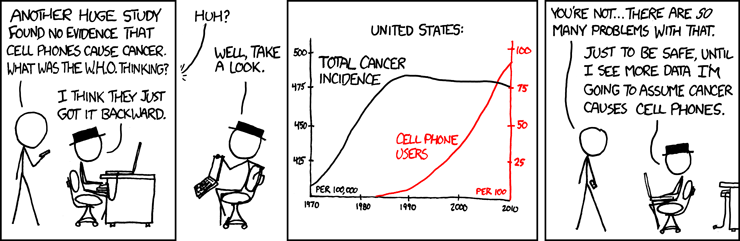
\includegraphics[width=0.6\linewidth,height=0.6\textheight]{figures/cellphonesxkcd} 

}

\caption{https://xkcd.com/925/}\label{fig:unnamed-chunk-1}
\end{figure}

\begin{center}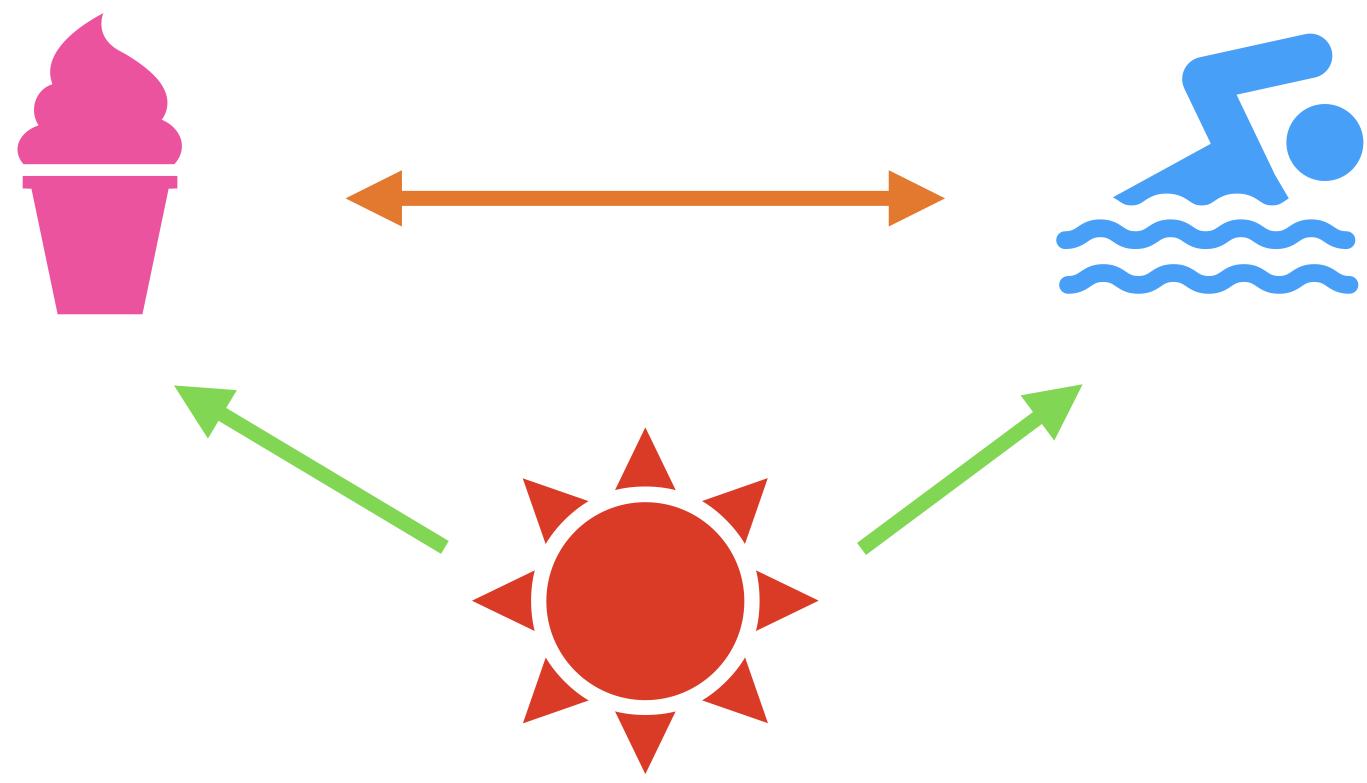
\includegraphics[width=0.4\linewidth,height=0.4\textheight]{figures/corr1} \end{center}

\hypertarget{simple-regression-introduction}{%
\section{Simple regression:
Introduction}\label{simple-regression-introduction}}

\hypertarget{motivation}{%
\subsection{Motivation}\label{motivation}}

\textbf{Predicting the Price of a used car}

\begin{center}
\includegraphics[width=0.6\linewidth,height=0.6\textheight]{figures/motivation1} \end{center}

\begin{center}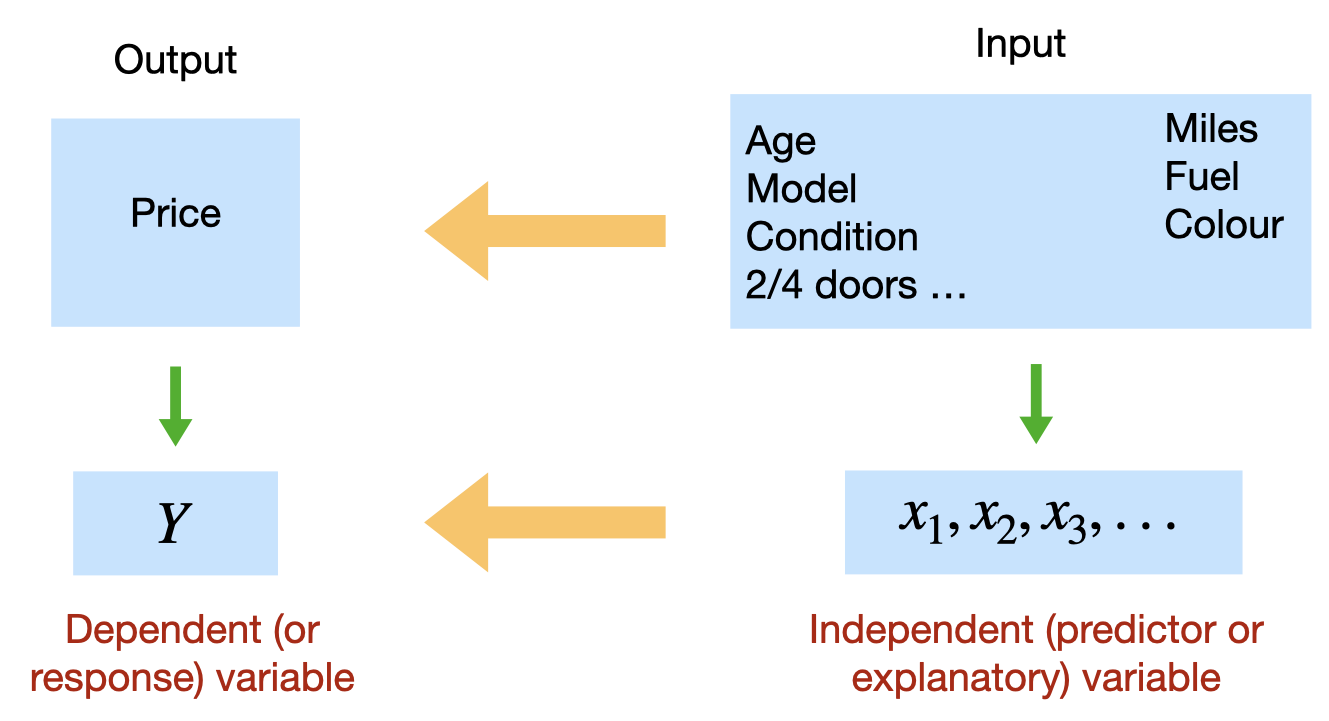
\includegraphics[width=0.6\linewidth,height=0.6\textheight]{figures/motivation2} \end{center}

\hypertarget{simple-linear-regression}{%
\subsection{Simple linear regression}\label{simple-linear-regression}}

\textbf{Simple linear regression (population)}
\[Y=\beta_0+\beta_1 x+\epsilon\] In our example:
\[Price=\beta_0+\beta_1 Age+\epsilon\]

\textbf{Simple linear regression (sample)} \[\hat{y}=b_0+b_1 x\] where
the coefficient \(\beta_0\) (and its estimate \(b_0\) or
\(\hat{\beta}_0\) ) refers to the \(y\)-intercept or simply the
intercept or the constant of the regression line, and the coefficient
\(\beta_1\) (and its estimate \(b_1\) or \(\hat{\beta}_1\) ) refers to
the slope of the regression line.

\hypertarget{least-squares-criterion}{%
\subsection{Least-Squares criterion}\label{least-squares-criterion}}

\begin{itemize}
\item
  The \textbf{least-squares criterion} is that the line that best fits a
  set of data points is the one having the smallest possible sum of
  squared errors. The `errors' are the vertical distances of the data
  points to the line.
\item
  We need to use the data to estimate the values of the parameters
  \(\beta_0\) and \(\beta_1\), i.e.~to fit a straight line to the set of
  points \(\{(x_i , y_i )\}\). There are many straight lines we could
  use, so we need some idea of which is best. Clearly, a bad straight
  line model would be one that had many large errors, and conversely, a
  good straight line model will have, on average, small errors. We
  quantify this by the sum of squares of the errors:
  \[Q(\beta_0,\beta_1)=\sum_{i=1}^n \epsilon_i^2=\sum_{i=1}^n[y_i-(\beta_0 + \beta_1 x_i)]^2\]
  then the ``line of best fit'' will correspond to the line with values
  of \(\beta_0\) and \(\beta_1\) that minimises \(Q(\beta_0,\beta_1)\).
\item
  The regression line is the line that fits a set of data points
  according to the least squares criterion.
\item
  The regression equation is the equation of the regression line.
\item
  The regression equation for a set of \(n\) data points is
  \(\hat{y}=b_0+b_1\;x\), where
  \[b_1=\frac{S_{xy}}{S_{xx}}=\frac{\sum (x_i-\bar{x})(y_i-\bar{y})}{\sum (x_i-\bar{x})^2}
   \;\;\text{and}\;\; b_0=\bar{y}-b_1\; \bar{x}\]
\item
  \(y\) is the dependent variable (or response variable) and \(x\) is
  the independent variable (predictor variable or explanatory variable).
\item
  \(b_0\) is called the \textbf{y-intercept} and \(b_1\) is called the
  \textbf{slope}.
\end{itemize}

\begin{center}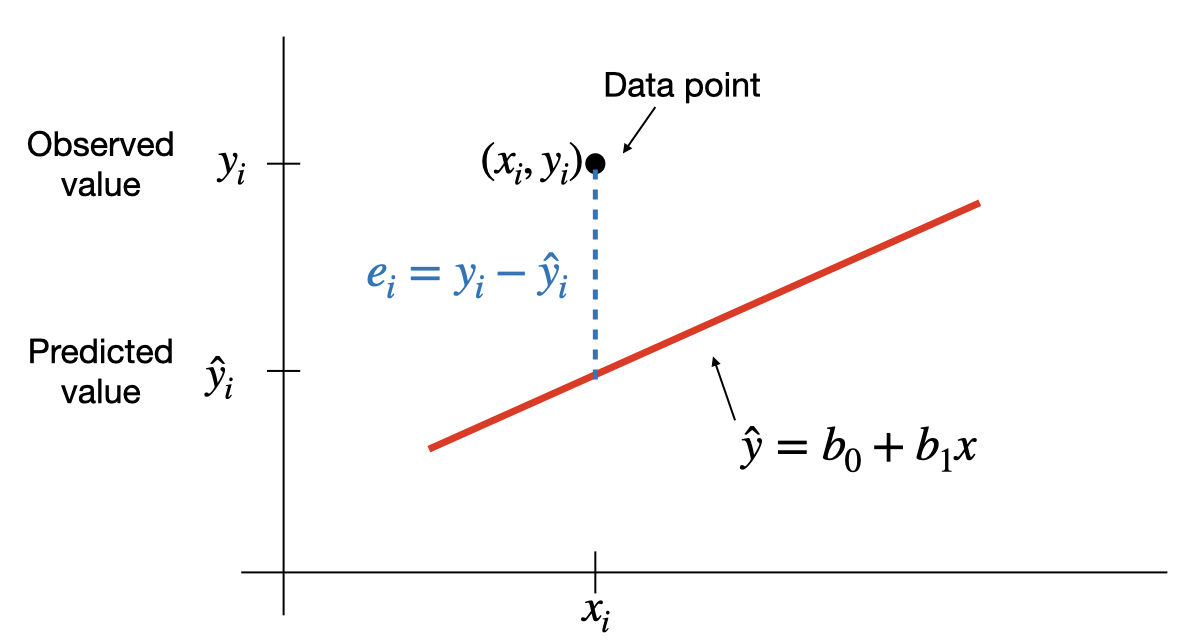
\includegraphics[width=0.6\linewidth,height=0.6\textheight]{figures/leastsq2} \end{center}

\textbf{SSE and the standard error}

This least square regression line minimizes the error sum of squares
\[SSE=\sum e^2_i =\sum (y_i-\hat{y}_i)^2\] The standard error of the
estimate, \(s_e=\sqrt{SSE/(n-2)}\), indicates how much, on average, the
observed values of the response variable differ from the predicated
values of the response variable.

\begin{center}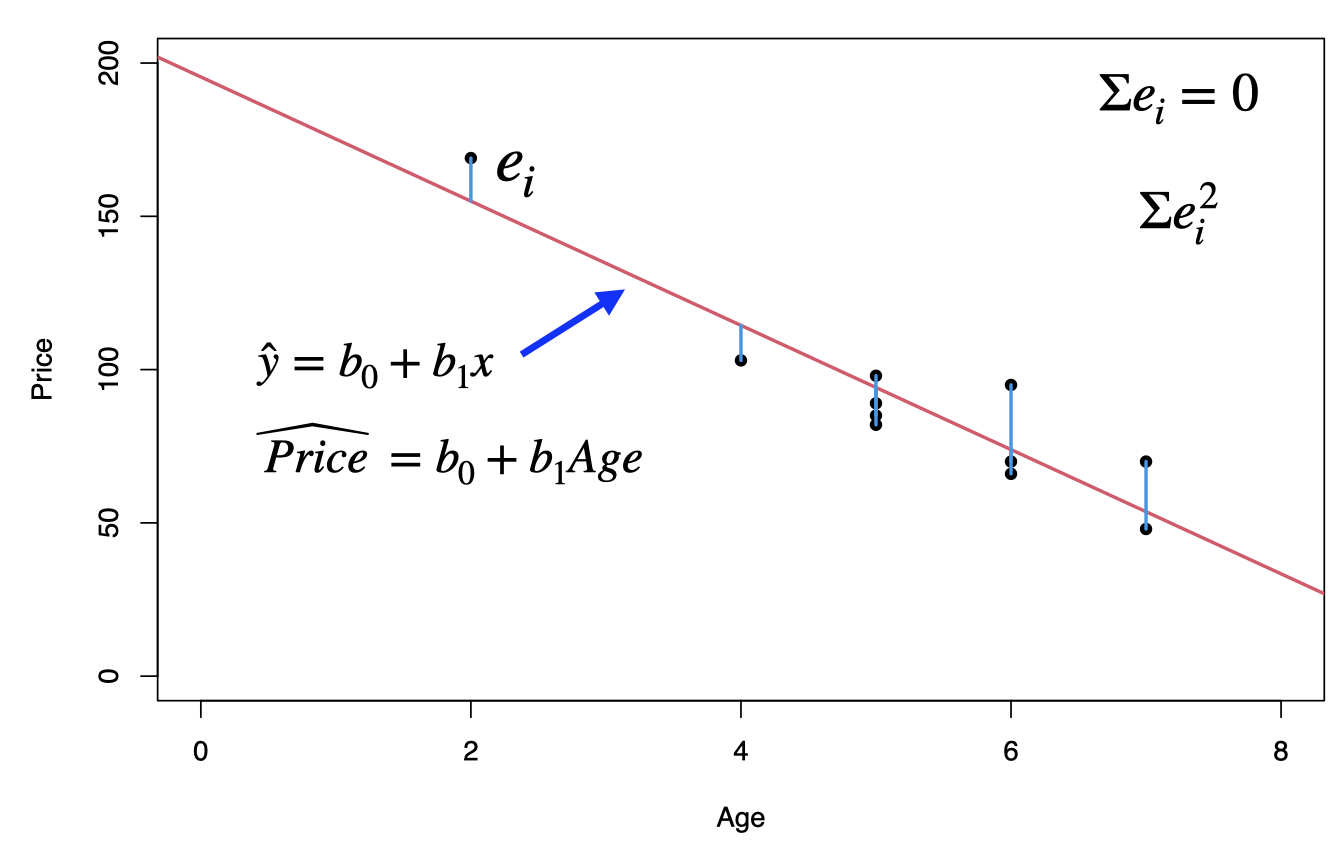
\includegraphics[width=0.6\linewidth,height=0.6\textheight]{figures/leastsq1} \end{center}

\hypertarget{example-used-cars-cont.}{%
\subsection{Example: used cars (cont.)}\label{example-used-cars-cont.}}

The table below displays data on Age (in years) and Price (in hundreds
of dollars) for a sample of cars of a particular make and model.(Weiss,
2012)

\begin{longtable}[]{@{}cc@{}}
\toprule\noalign{}
Price (\(y\)) & Age (\(x\)) \\
\midrule\noalign{}
\endhead
\bottomrule\noalign{}
\endlastfoot
85 & 5 \\
103 & 4 \\
70 & 6 \\
82 & 5 \\
89 & 5 \\
98 & 5 \\
66 & 6 \\
95 & 6 \\
169 & 2 \\
70 & 7 \\
48 & 7 \\
\end{longtable}

\begin{itemize}
\item
  For our example, \emph{age} is the predictor variable and \emph{price}
  is the response variable.
\item
  The regression equation is \(\hat{y}=195.47-20.26\;x\), where the
  slope \(b_1=-20.26\) and the intercept \(b_0=195.47\)
\item
  Prediction: for \(x = 4\), that is we would like to predict the price
  of a 4-year-old car,
  \[\hat{y}=195.47-20.26 {\color{blue}(4)}= 114.43 \;\;\text{or}\;\; \$ 11443\]
\end{itemize}

\begin{center}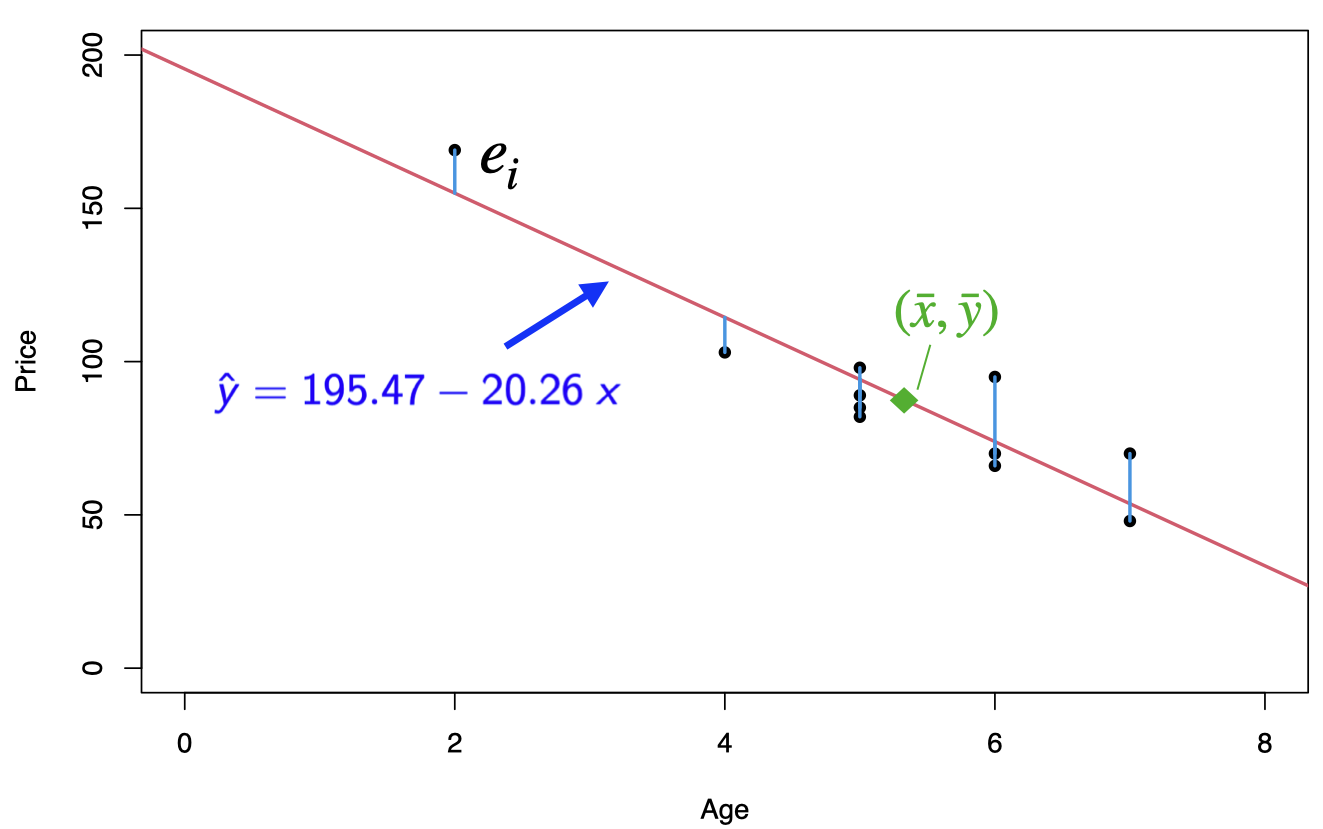
\includegraphics[width=0.6\linewidth,height=0.6\textheight]{figures/leastsq5} \end{center}

Back to our used cars example, we want to find the ``best line'' through
the data points, which can be used to predict prices of used cars based
on their age.

First we need to enter the data in R.

\begin{Shaded}
\begin{Highlighting}[]
\NormalTok{Price}\OtherTok{\textless{}{-}}\FunctionTok{c}\NormalTok{(}\DecValTok{85}\NormalTok{, }\DecValTok{103}\NormalTok{,  }\DecValTok{70}\NormalTok{,  }\DecValTok{82}\NormalTok{,  }\DecValTok{89}\NormalTok{,  }\DecValTok{98}\NormalTok{,  }\DecValTok{66}\NormalTok{,  }\DecValTok{95}\NormalTok{, }\DecValTok{169}\NormalTok{,  }\DecValTok{70}\NormalTok{,  }\DecValTok{48}\NormalTok{)}
\NormalTok{Age}\OtherTok{\textless{}{-}} \FunctionTok{c}\NormalTok{(}\DecValTok{5}\NormalTok{, }\DecValTok{4}\NormalTok{, }\DecValTok{6}\NormalTok{, }\DecValTok{5}\NormalTok{, }\DecValTok{5}\NormalTok{, }\DecValTok{5}\NormalTok{, }\DecValTok{6}\NormalTok{, }\DecValTok{6}\NormalTok{, }\DecValTok{2}\NormalTok{, }\DecValTok{7}\NormalTok{, }\DecValTok{7}\NormalTok{)}
\NormalTok{carSales}\OtherTok{\textless{}{-}}\FunctionTok{data.frame}\NormalTok{(Price,Age)}
\FunctionTok{str}\NormalTok{(carSales)}
\end{Highlighting}
\end{Shaded}

\begin{verbatim}
## 'data.frame':    11 obs. of  2 variables:
##  $ Price: num  85 103 70 82 89 98 66 95 169 70 ...
##  $ Age  : num  5 4 6 5 5 5 6 6 2 7 ...
\end{verbatim}

\begin{Shaded}
\begin{Highlighting}[]
\FunctionTok{cor}\NormalTok{(Age, Price, }\AttributeTok{method =} \StringTok{"pearson"}\NormalTok{)}
\end{Highlighting}
\end{Shaded}

\begin{verbatim}
## [1] -0.9237821
\end{verbatim}

Scatterplot: Age vs.~Price

\begin{Shaded}
\begin{Highlighting}[]
\FunctionTok{library}\NormalTok{(ggplot2)}
\end{Highlighting}
\end{Shaded}

\begin{verbatim}
## Warning: package 'ggplot2' was built under R version 4.3.2
\end{verbatim}

\begin{Shaded}
\begin{Highlighting}[]
\FunctionTok{ggplot}\NormalTok{(carSales, }\FunctionTok{aes}\NormalTok{(}\AttributeTok{x=}\NormalTok{Age, }\AttributeTok{y=}\NormalTok{Price)) }\SpecialCharTok{+} \FunctionTok{geom\_point}\NormalTok{()}
\end{Highlighting}
\end{Shaded}
 
\begin{center}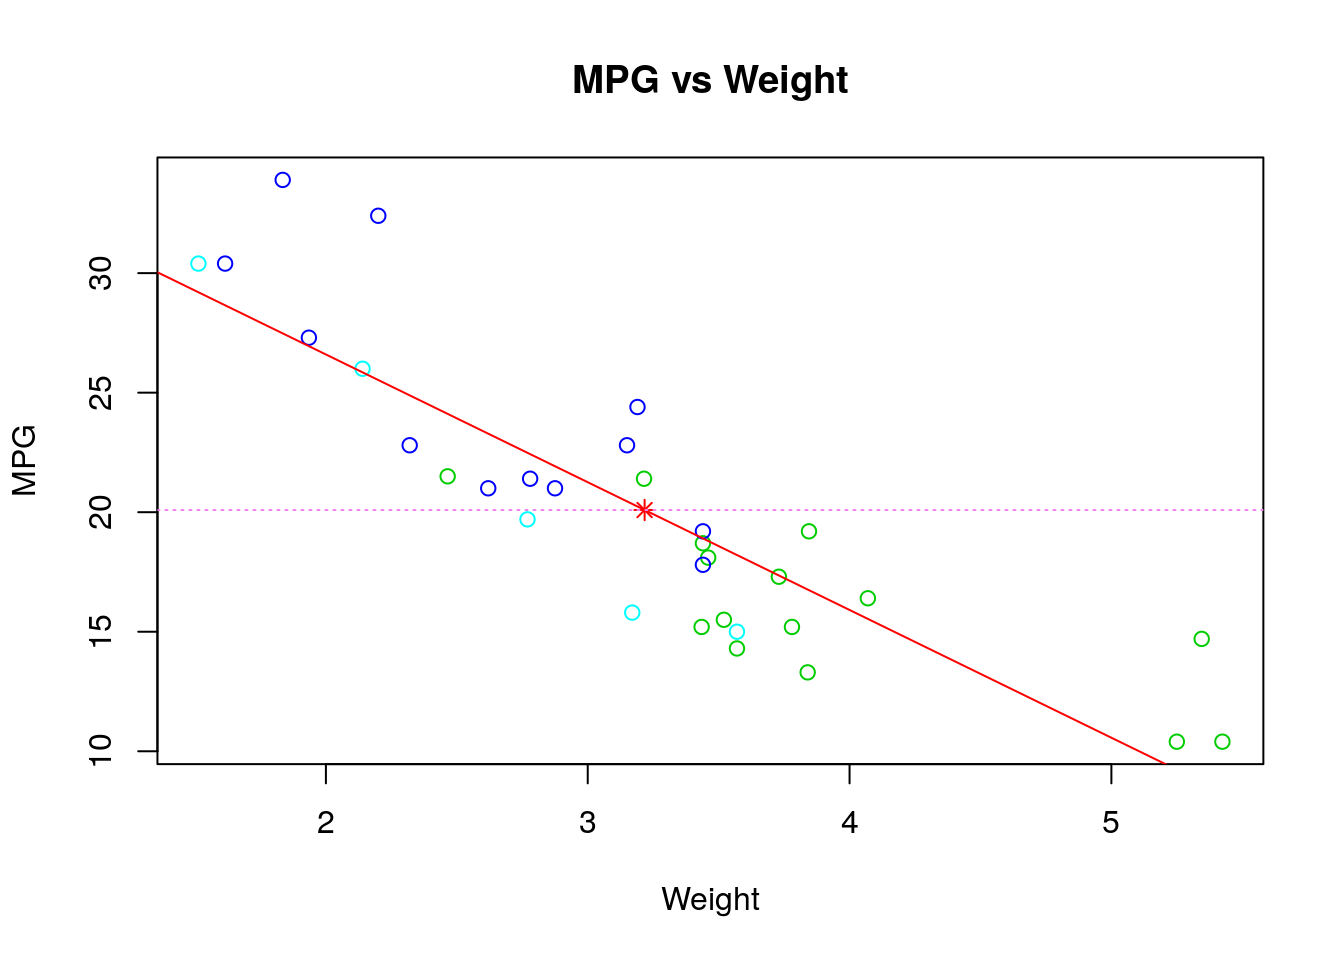
\includegraphics[width=0.5\linewidth,height=0.5\textheight]{unnamed-chunk-9-1} \end{center}

\begin{Shaded}
\begin{Highlighting}[]
\CommentTok{\# Remove the confidence interval}
\FunctionTok{ggplot}\NormalTok{(carSales, }\FunctionTok{aes}\NormalTok{(}\AttributeTok{x=}\NormalTok{Age, }\AttributeTok{y=}\NormalTok{Price)) }\SpecialCharTok{+} 
  \FunctionTok{geom\_point}\NormalTok{()}\SpecialCharTok{+}
  \FunctionTok{geom\_smooth}\NormalTok{(}\AttributeTok{method=}\NormalTok{lm, }\AttributeTok{formula=}\NormalTok{ y}\SpecialCharTok{\textasciitilde{}}\NormalTok{x, }\AttributeTok{se=}\ConstantTok{FALSE}\NormalTok{)}
\end{Highlighting}
\end{Shaded}

\begin{center}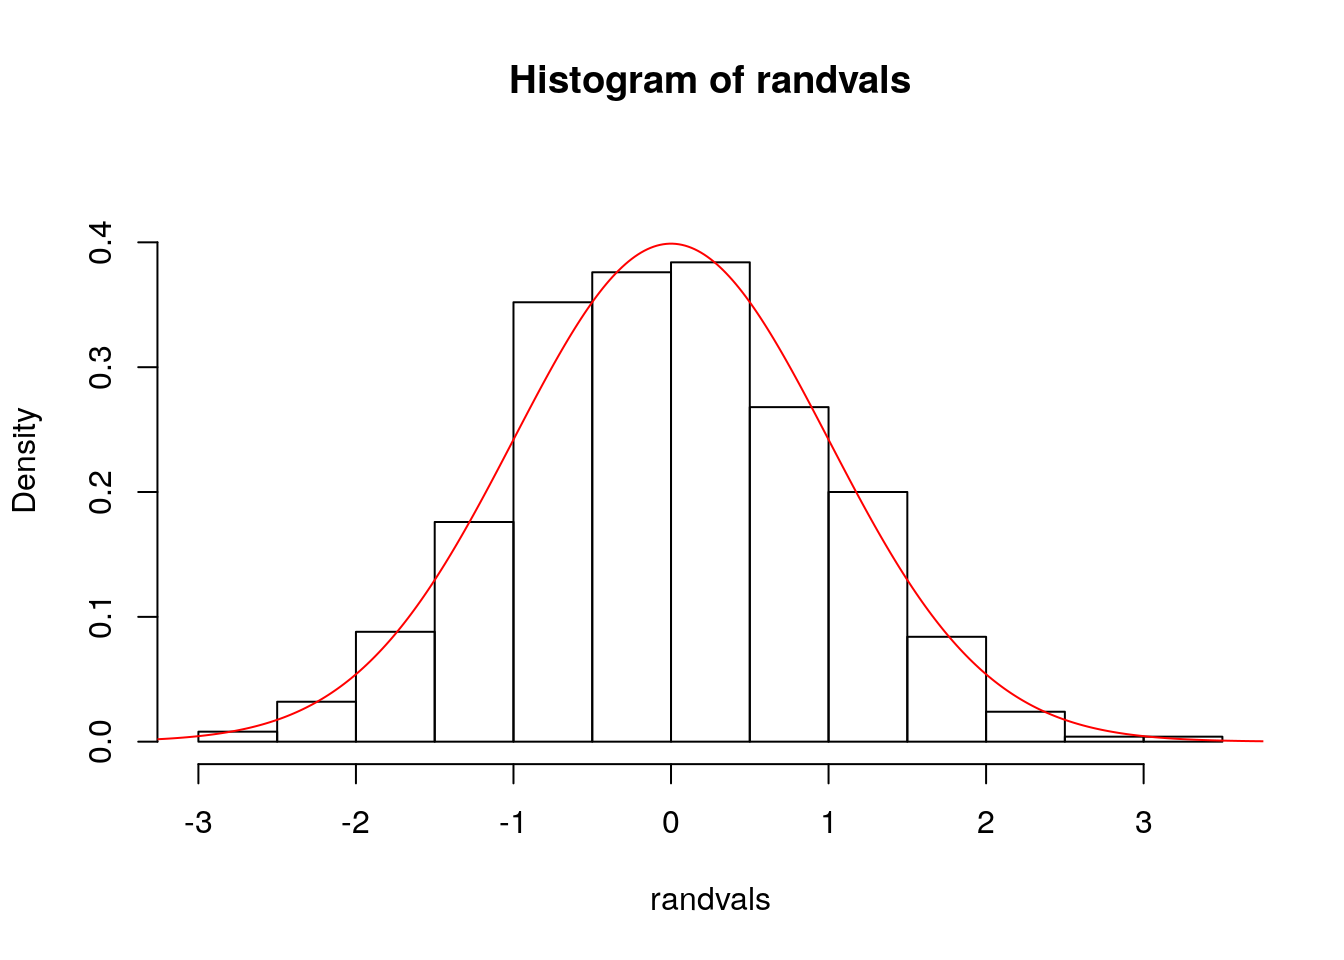
\includegraphics[width=0.5\linewidth,height=0.5\textheight]{unnamed-chunk-10-1} \end{center}

\hypertarget{prediction}{%
\subsection{Prediction}\label{prediction}}

\begin{Shaded}
\begin{Highlighting}[]
\CommentTok{\# simple linear regression}
\NormalTok{reg}\OtherTok{\textless{}{-}}\FunctionTok{lm}\NormalTok{(Price}\SpecialCharTok{\textasciitilde{}}\NormalTok{Age)}
\FunctionTok{print}\NormalTok{(reg)}
\end{Highlighting}
\end{Shaded}

\begin{verbatim}
## 
## Call:
## lm(formula = Price ~ Age)
## 
## Coefficients:
## (Intercept)          Age  
##      195.47       -20.26
\end{verbatim}

To predict the price of a 4-year-old car (\(x=4\)):
\[\hat{y}=195.47-20.26(4)=114.43\]

\begin{center}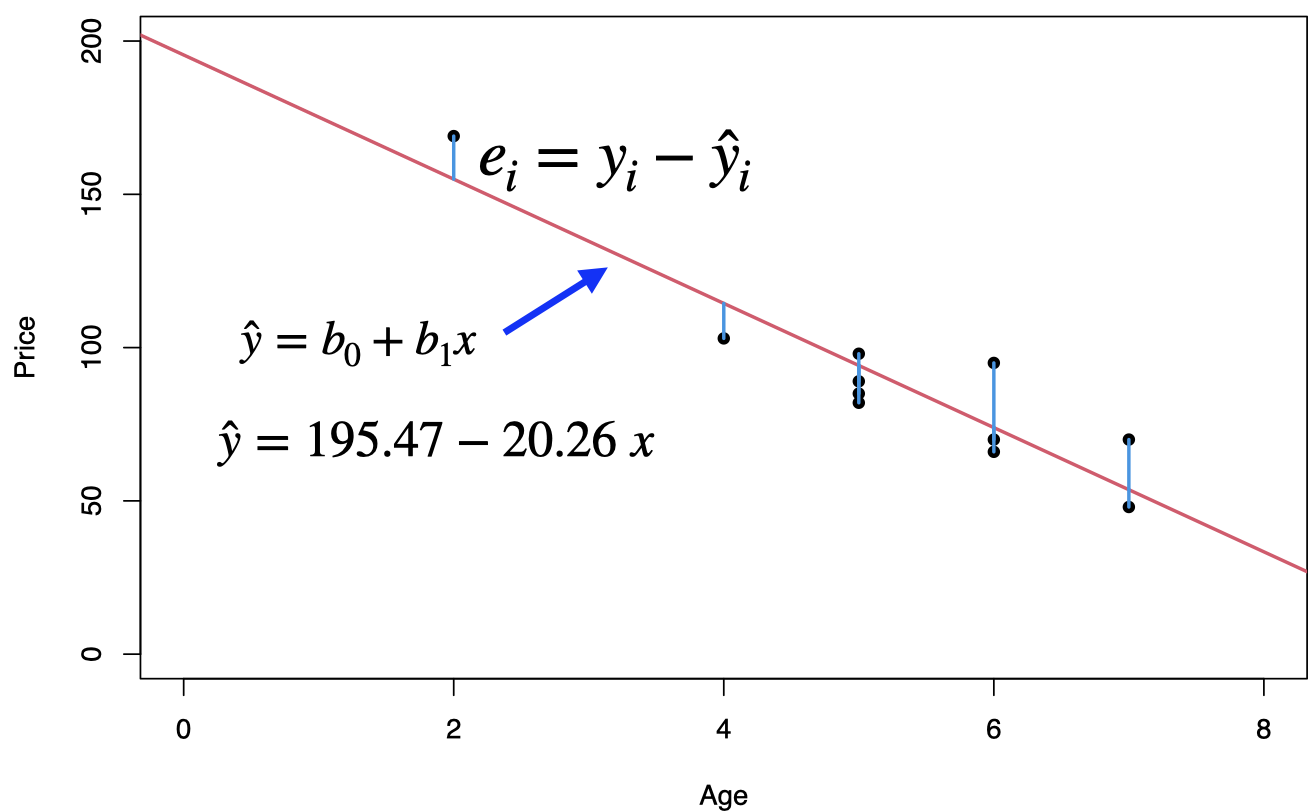
\includegraphics[width=0.6\linewidth,height=0.6\textheight]{figures/leastsq3} \end{center}

\hypertarget{simple-regression-coefficient-of-determination}{%
\section{Simple Regression: Coefficient of
Determination}\label{simple-regression-coefficient-of-determination}}

\hypertarget{extrapolation}{%
\subsection{Extrapolation}\label{extrapolation}}

\begin{itemize}
\item
  Within the range of the observed values of the predictor variable, we
  can reasonably use the regression equation to make predictions for the
  response variable.
\item
  However, to do so outside the range, which is called
  \textbf{Extrapolation}, may not be reasonable because the linear
  relationship between the predictor and response variables may not hold
  here.
\item
  To predict the price of an 11-year old car,
  \(\hat{y}=195.47-20.26 (11)=-27.39\) or \$ 2739, this result is
  unrealistic as no one is going to pay us \$2739 to take away their
  11-year old car.
\end{itemize}

\begin{center}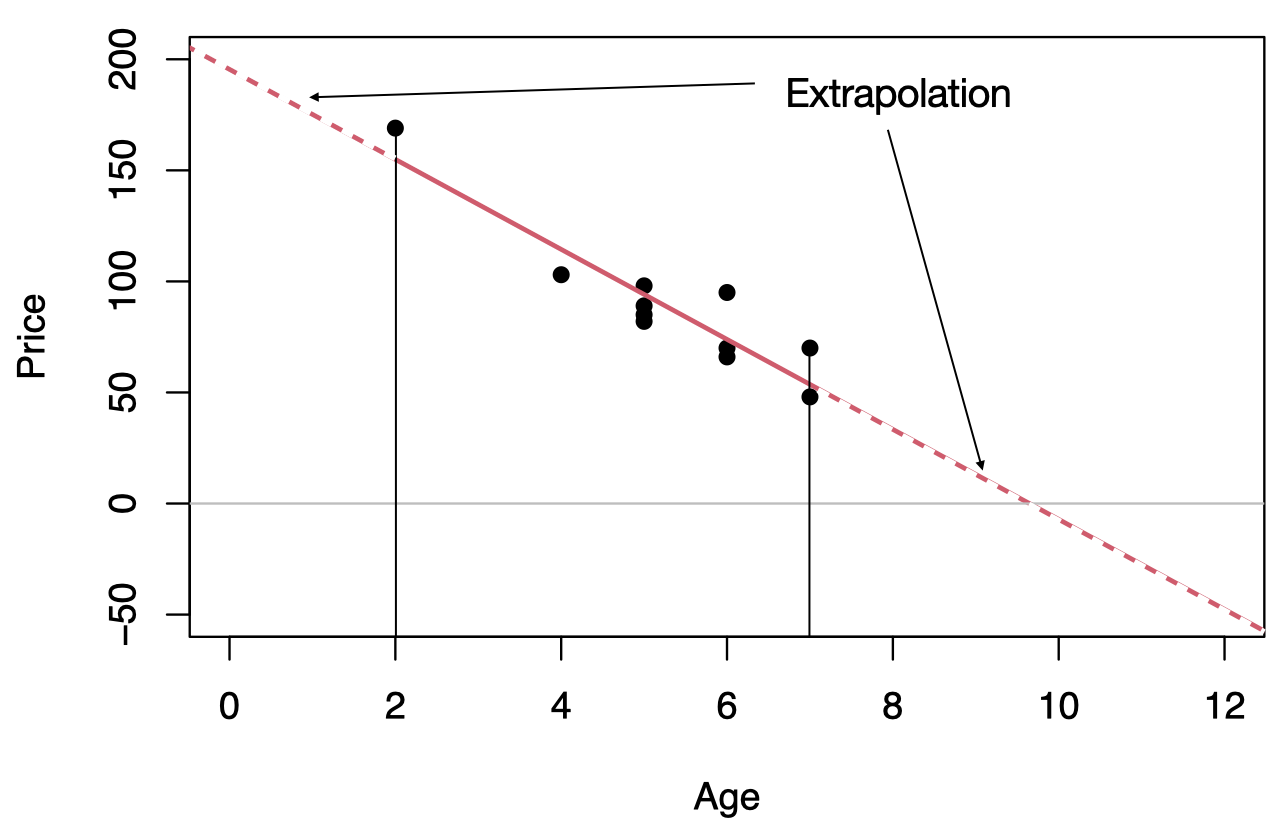
\includegraphics[width=0.6\linewidth,height=0.6\textheight]{figures/extrap} \end{center}

\hypertarget{outliers-and-influential-observations}{%
\subsection{Outliers and influential
observations}\label{outliers-and-influential-observations}}

\begin{itemize}
\item
  Recall that an \textbf{outlier} is an observation that lies outside
  the overall pattern of the data. In the context of regression, an
  outlier is a data point that lies far from the regression line,
  relative to the other data points.
\item
  An \textbf{influential observation} is a data point whose removal
  causes the regression equation (and line) to change considerably.
\item
  From the scatterplot, it seems that the data point (2,169) might be an
  influential observation. Removing that data point and recalculating
  the regression equation yields \(\hat{y}=160.33-14.24\;x\).
\end{itemize}

\begin{center}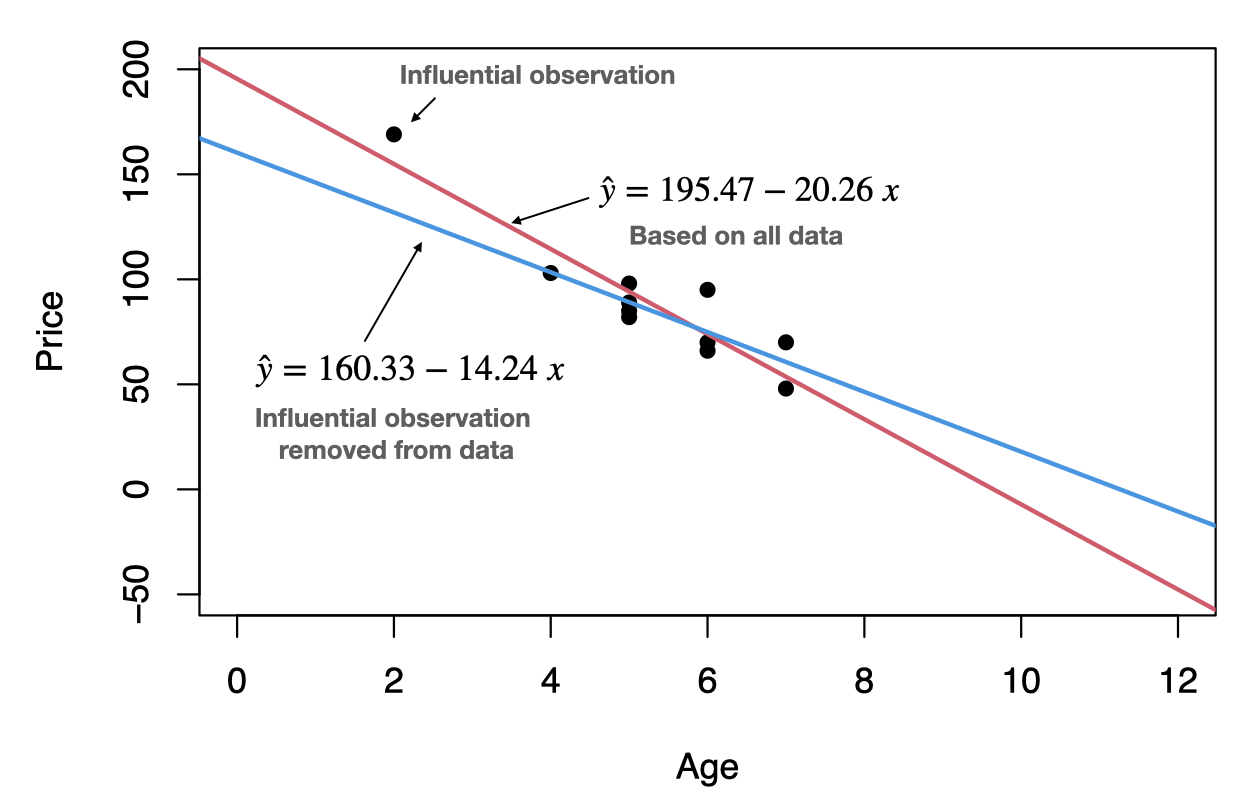
\includegraphics[width=0.6\linewidth,height=0.6\textheight]{figures/outliersreg} \end{center}

\hypertarget{coefficient-of-determination}{%
\subsection{Coefficient of
determination}\label{coefficient-of-determination}}

\begin{center}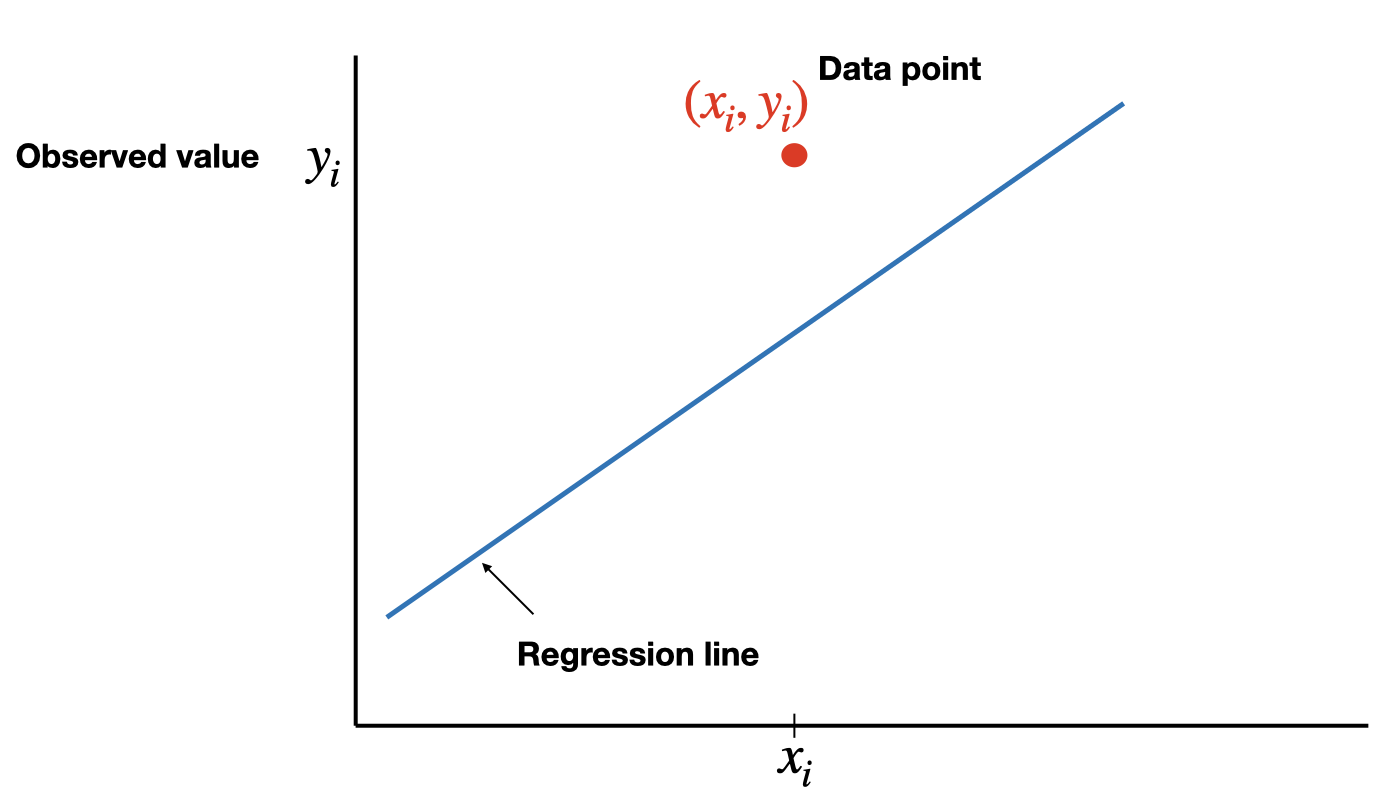
\includegraphics[width=0.6\linewidth,height=0.6\textheight]{figures/cod1} \end{center}

\begin{center}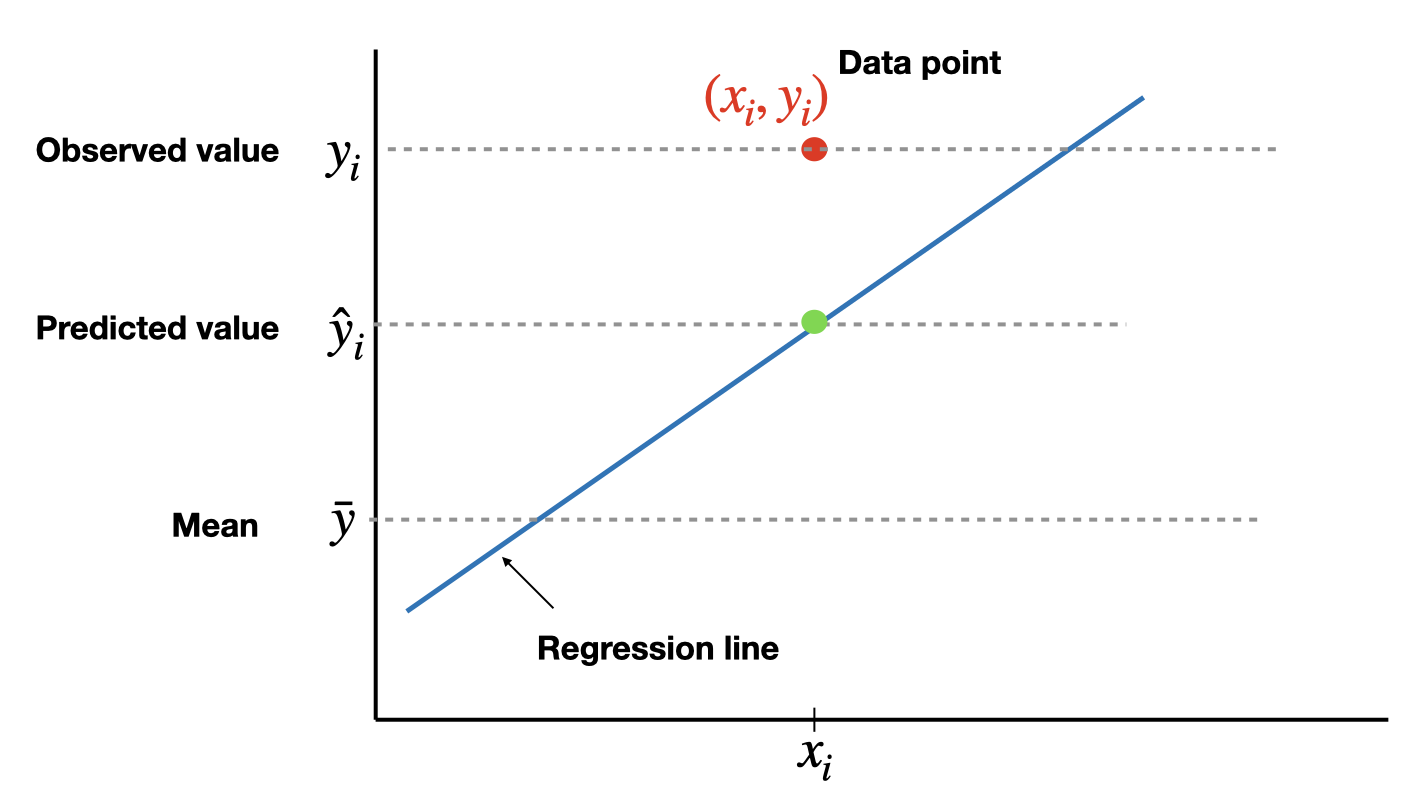
\includegraphics[width=0.6\linewidth,height=0.6\textheight]{figures/cod2} \end{center}

\begin{center}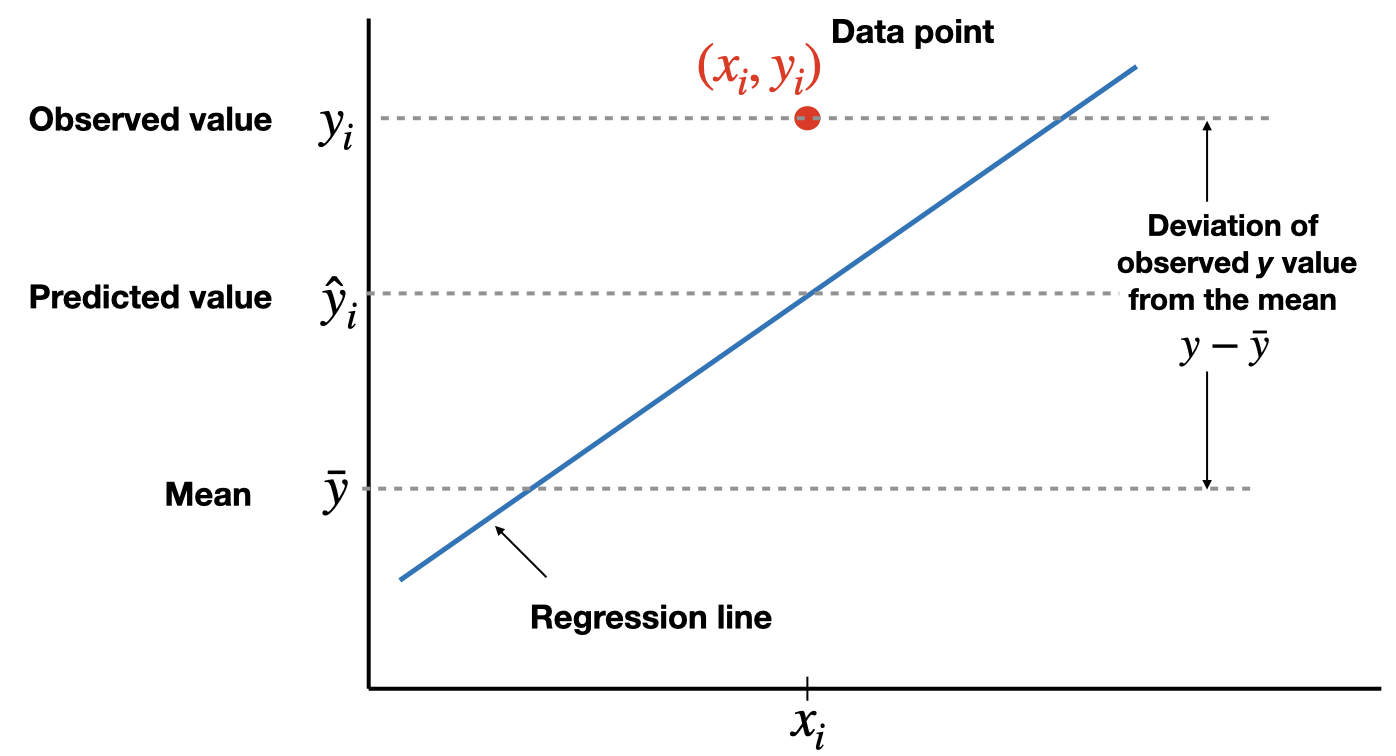
\includegraphics[width=0.6\linewidth,height=0.6\textheight]{figures/cod3} \end{center}

\begin{center}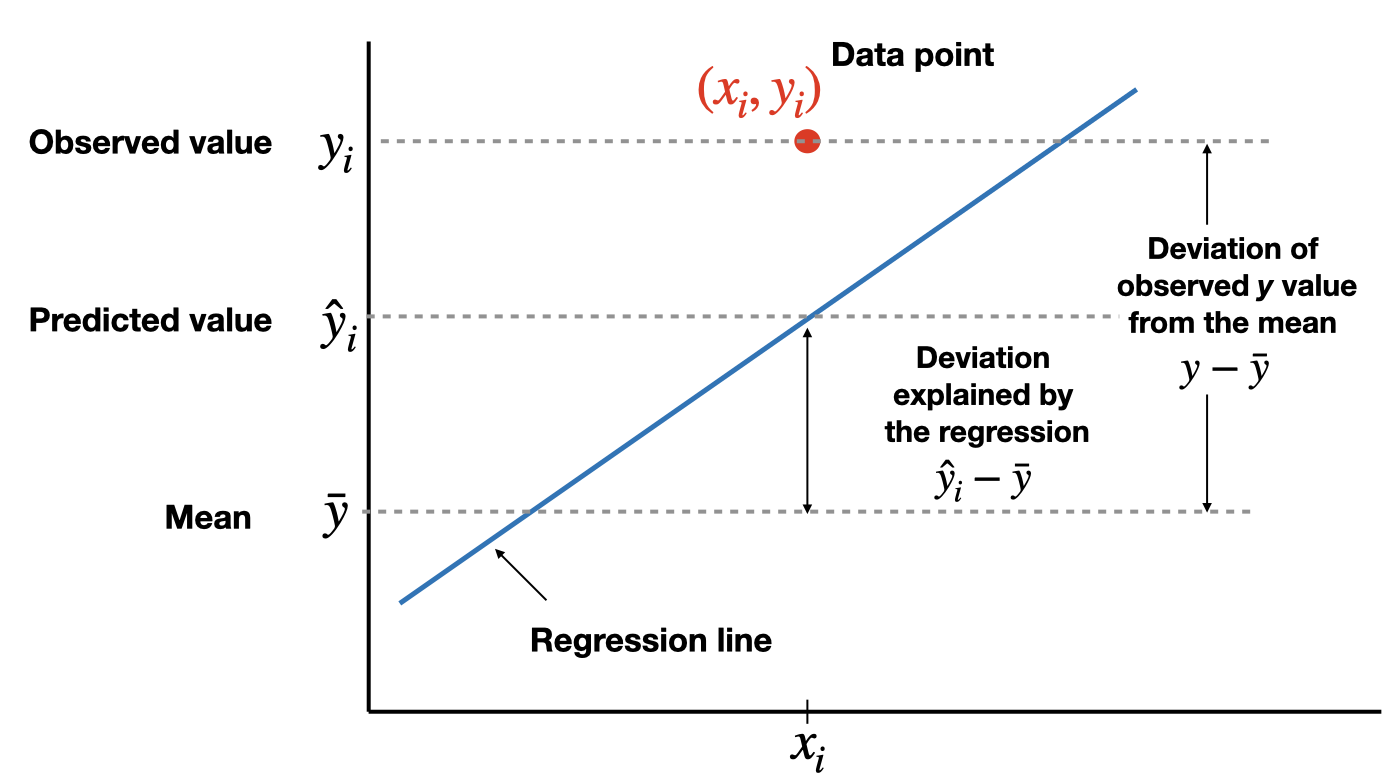
\includegraphics[width=0.6\linewidth,height=0.6\textheight]{figures/cod4} \end{center}

\begin{center}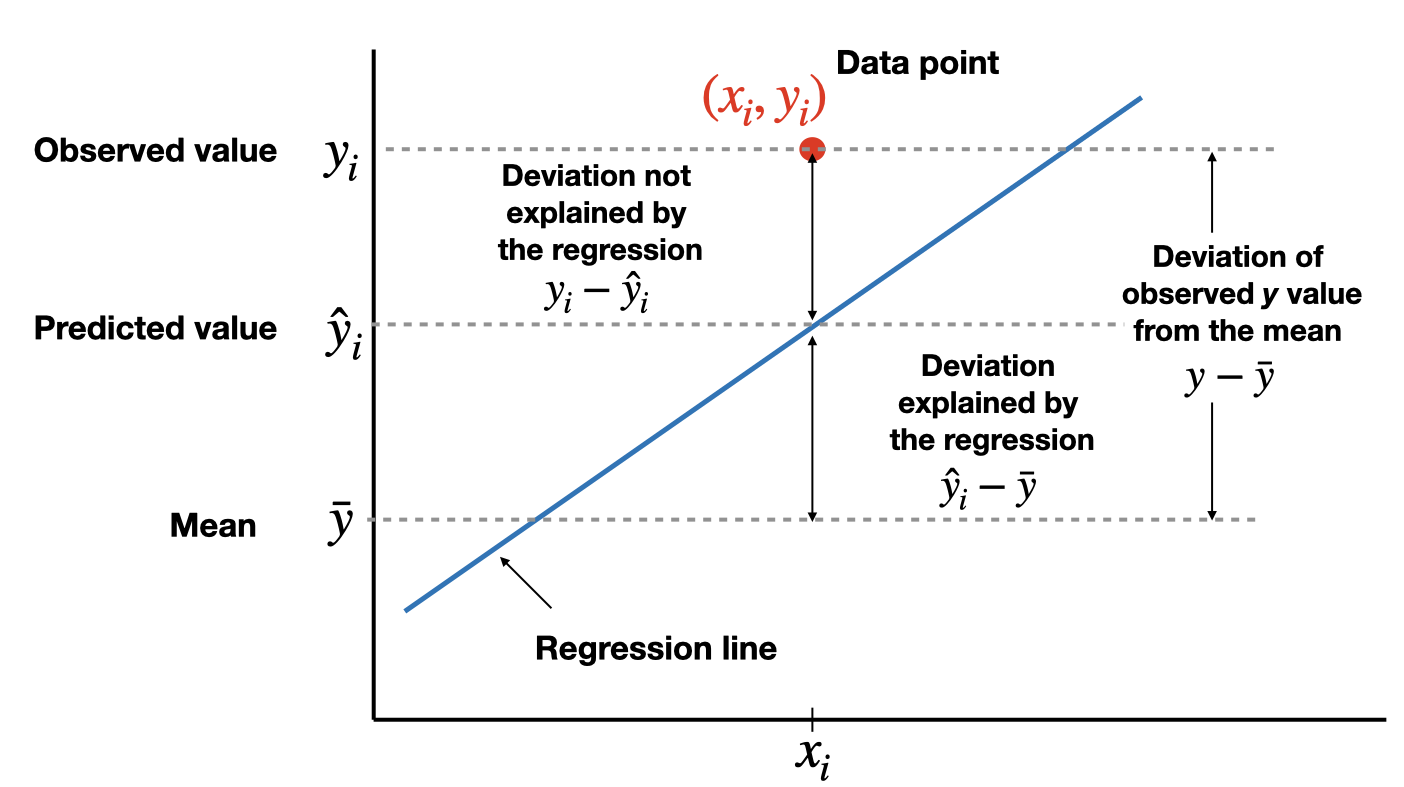
\includegraphics[width=0.6\linewidth,height=0.6\textheight]{figures/cod5} \end{center}

\begin{itemize}
\item
  The total variation in the observed values of the response variable,
  \(SST=\sum(y_i-\bar{y})^2\), can be partitioned into two components:

  \begin{itemize}
  \tightlist
  \item
    The variation in the observed values of the response variable
    explained by the regression: \(SSR=\sum(\hat{y}_i-\bar{y})^2\)
  \item
    The variation in the observed values of the response variable not
    explained by the regression: \(SSE=\sum(y_i-\hat{y}_i)^2\)
  \end{itemize}
\item
  The coefficient of determination, \(R^2\) (or \(R\)-square), is the
  proportion of the variation in the observed values of the response
  variable explained by the regression, which is given by
  \[R^2=\frac{SSR}{SST}=\frac{SST-SSE}{SST}=1-\frac{SSE}{SST}\] where
  \(SST=SSR+SSE\). \(R^2\) is a descriptive measure of the utility of
  the regression equation for making prediction.
\item
  The coefficient of determination \(R^2\) always lies between 0 and 1.
  A value of \(R^2\) near 0 suggests that the regression equation is not
  very useful for making predictions, whereas a value of \(R^2\) near 1
  suggests that the regression equation is quite useful for making
  predictions.
\item
  For a simple linear regression (one independent variable) ONLY,
  \(R^2\) is the square of Pearson correlation coefficient, \(r\).
\item
  \(\text{Adjusted}\;R^2\) is a modification of \(R^2\) which takes into
  account the number of independent variables, say \(k\). In a simple
  linear regression \(k=1\). Adjusted-\(R^2\) increases only when a
  significant related independent variable is added to the model.
  Adjusted-\(R^2\) has a crucial role in the process of model building.
  Adjusted-\(R^2\) is given by
  \[\text{Adjusted-}R^2=1-(1-R^2)\frac{n-1}{n-k-1}\]
\end{itemize}

\hypertarget{notation-used-in-regression}{%
\subsection{Notation used in
regression}\label{notation-used-in-regression}}

\begin{longtable}[]{@{}ccl@{}}
\toprule\noalign{}
Quantity & Defining formula & Computing formula \\
\midrule\noalign{}
\endhead
\bottomrule\noalign{}
\endlastfoot
\(S_{xx}\) & \(\sum (x_i-\bar{x})^2\) & \(\sum x^2_i - n \bar{x}^2\) \\
\(S_{xy}\) & \(\sum (x_i-\bar{x})(y_i-\bar{y})\) &
\(\sum x_i y_i - n \bar{x}\bar{y}\) \\
\(S_{yy}\) & \(\sum (y_i-\bar{y})^2\) & \(\sum y^2_i - n \bar{y}^2\) \\
\end{longtable}

where \(\bar{x}=\frac{\sum x_i}{n}\) and \(\bar{y}=\frac{\sum y_i}{n}\).
And,

\[SST=S_{yy},\;\;\; SSR=\frac{S^2_{xy}}{S_{xx}},\;\;\; SSE=S_{yy}-\frac{S^2_{xy}}{S_{xx}} \]
and \(SST=SSR+SSE\).

\hypertarget{pearson-correlation-coefficient}{%
\subsection{Pearson correlation
coefficient}\label{pearson-correlation-coefficient}}

\textbf{Pearson correlation coefficient} (\(r\)) is a measure of the
strength and the direction of \textbf{a linear relationship} between two
variables in the sample,

\[r=\frac{\sum(x_{i} -\bar{x})(y_{i} -\bar{y}) }{\sqrt{\sum (x_{i} -\bar{x})^{2}  \sum (y_{i} -\bar{y})^{2}  } } \]

where \(r\) always lies between -1 and 1. Values of \(r\) near -1 or 1
indicate a strong linear relationship between the variables whereas
values of \(r\) near 0 indicate a weak linear relationship between
variables. If \(r\) is zero the variables are linearly uncorrelated,
that is there is no linear relationship between the two variables.

\begin{center}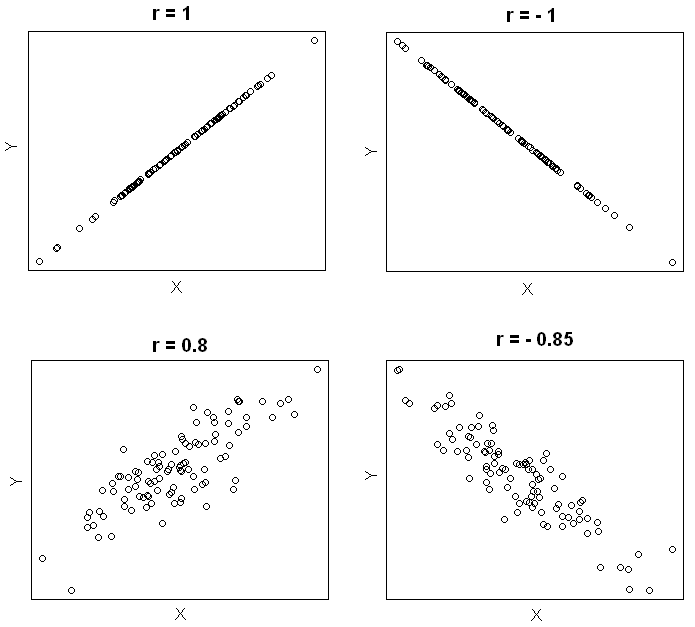
\includegraphics[width=0.6\linewidth,height=0.6\textheight]{figures/rr1} \end{center}

\begin{center}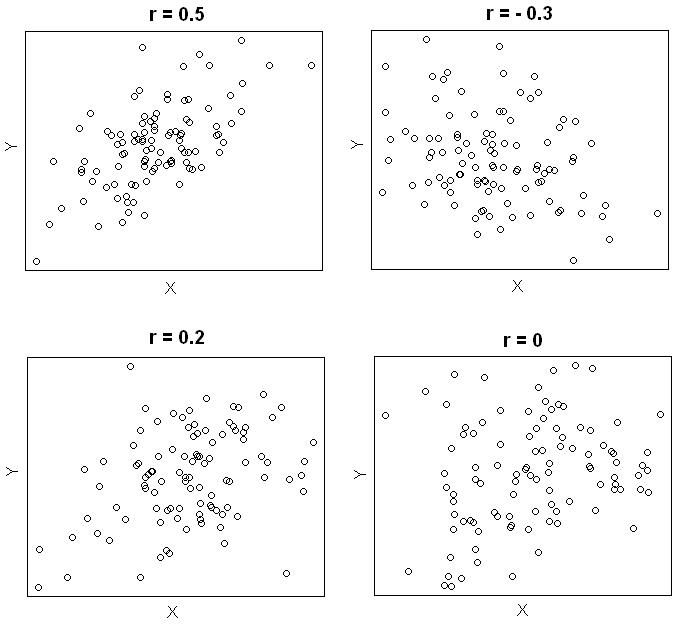
\includegraphics[width=0.6\linewidth,height=0.6\textheight]{figures/rr2} \end{center}

\begin{center}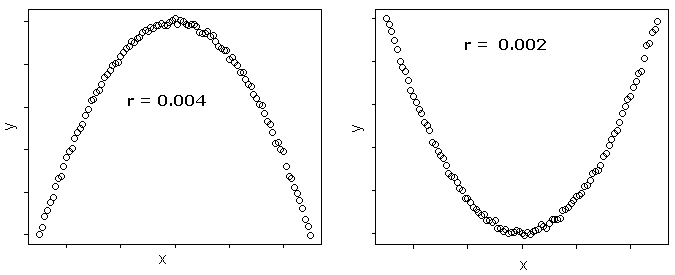
\includegraphics[width=0.6\linewidth,height=0.6\textheight]{figures/corr0} \end{center}

\hypertarget{hypothesis-testing-for-the-population-correlation-coefficient-rho}{%
\subsection{\texorpdfstring{Hypothesis testing for the population
correlation coefficient
\(\rho\)}{Hypothesis testing for the population correlation coefficient \textbackslash rho}}\label{hypothesis-testing-for-the-population-correlation-coefficient-rho}}

Hypothesis testing for the population correlation coefficient \(\rho\).

Assumptions:

\begin{itemize}
\tightlist
\item
  The sample of paired \((x, y)\) data is a random sample.
\item
  The pairs of \((x, y)\) data have a bivariate normal distribution.
\end{itemize}

The null hypothesis

\(H_0: \rho = 0\) (no significant correlation)

against one of the alternative hypotheses:

\begin{itemize}
\item
  \(H_1: \rho \neq 0\) (significant correlation) ``Two-tailed test'\,'
\item
  \(H_1: \rho < 0\) (significant negative correlation) ``Left-tailed
  test'\,'
\item
  \(H_1: \rho > 0\) (significant positive correlation) ``Right-tailed
  test'\,'
\end{itemize}

Compute the value of the test statistic:
\[t=\frac{r\; \sqrt{n-2} }{\sqrt{1-r^{2} } }\sim T_{(n-2)} \;\; \text{with}\;\; df = n-2. \]

where \(n\) is the sample size.

The critical value(s) for this test can be found from T distribution
table ( \(\pm t_{\alpha/2}\) for a two-tailed test, \(- t_{\alpha}\) for
a left-tailed test and \(t_{\alpha}\) for a right-tailed test).

\begin{center}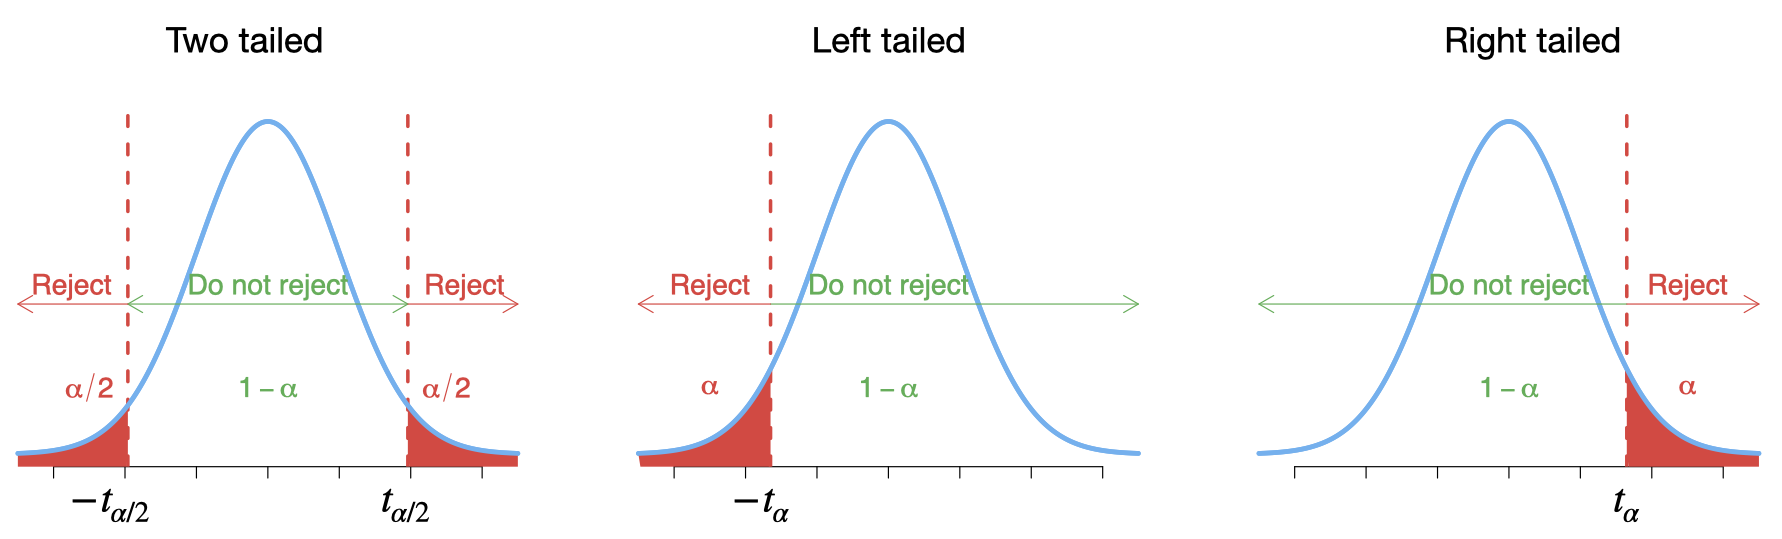
\includegraphics[width=0.8\linewidth,height=0.8\textheight]{figures/hypottest} \end{center}

\begin{itemize}
\tightlist
\item
  If the value of the test statistic falls in the rejection region, then
  reject \(H_0\); otherwise, do not reject \(H_0\).
\item
  Statistical packages report \textbf{p-values} rather than critical
  values which can be used in testing the null hypothesis \(H_0\).
\end{itemize}

\hypertarget{correlation-and-linear-transformation}{%
\subsection{Correlation and linear
transformation}\label{correlation-and-linear-transformation}}

\begin{itemize}
\item
  Suppose we have a linear transformation of the two variables \(x\) and
  \(y\), say \(x_1=a x+b\) and \(y_1=cy+d\) where \(a>0\) and \(c>0\).
  Then the Pearson correlation coefficient between \(x_1\) and \(y_1\)
  is equal to Pearson correlation coefficient between \(x\) and \(y\).
\item
  For our example, suppose we convert cars' prices from dollars to
  pounds (say \(\$1=\) \textsterling 0.75, so \(y_1=0.75 y\)), and we
  left the age of the cars unchanged. Then we will find that the
  correlation between the age of the car and its price in pounds is
  equal to the one we obtained before (i.e.~the correlation between the
  age and the price in dollars).
\item
  A special linear transformation is to standardize one or both
  variables. That is obtaining the values \(z_x=(x-\bar{x})/s_x\) and
  \(z_y=(y-\bar{y})/s_y\). Then the correlation between \(z_x\) and
  \(z_y\) is equal to the correlation between \(x\) and \(y\).
\end{itemize}

\hypertarget{spearmans-rho-correlation-coefficient-r_s}{%
\subsection{\texorpdfstring{Spearman's rho correlation coefficient
(\(r_s\))}{Spearman's rho correlation coefficient (r\_s)}}\label{spearmans-rho-correlation-coefficient-r_s}}

\begin{itemize}
\item
  When the normality assumption for the Pearson correlation coefficient
  \(r\) cannot be met, or when one or both variables may be ordinal,
  then we should consider nonparametric methods such as Spearman's rho
  and Kendall's tau correlation coefficients.
\item
  Spearman's rho correlation coefficient, \(r_s\),can be obtained by
  first rank the \(x\) values (and \(y\) values) among themselves, and
  then we compute the Pearson correlation coefficient of the rank pairs.
  Similarly \(-1\leq r_s \leq 1\), the values of \(r_s\) range from -1
  to +1 inclusive.
\item
  Spearman's rho correlation coefficient can be used to describe the
  strength of the linear relationship as well as the nonlinear
  relationship.
\end{itemize}

\hypertarget{kendalls-tau-tau-correlation-coefficient}{%
\subsection{\texorpdfstring{Kendall's tau (\(\tau\)) correlation
coefficient}{Kendall's tau (\textbackslash tau) correlation coefficient}}\label{kendalls-tau-tau-correlation-coefficient}}

\begin{itemize}
\item
  Kendall's tau, \(\tau\), measures the concordance of the relationship
  between two variables, and \(-1\leq \tau \leq 1\).
\item
  Any pair of observations \((x_i, y_i)\) and \((x_j, y_j)\) are said to
  be concordant if both \(x_i > x_j\) and \(y_i > y_j\) or if both
  \(x_i < x_j\) and \(y_i < y_j\). And they are said to be discordant,
  if \(x_i > x_j\) and \(y_i < y_j\) or if \(x_i < x_j\) and
  \(y_i > y_j\). We will have \(n(n-1)/2\) of pairs to compare.
\item
  The Kendall's tau (\(\tau\)) correlation coefficient is defined as:
  \[\tau=\frac{\text{number of concordant pairs} - \text{number of discordant pairs}}{n(n-1)/2}\]
\end{itemize}

\hypertarget{example-used-cars}{%
\subsection{Example: used cars}\label{example-used-cars}}

The table below displays data on Age (in years) and Price (in hundreds
of dollars) for a sample of cars of a particular make and model (Weiss,
2012).

\begin{longtable}[]{@{}cc@{}}
\toprule\noalign{}
Price (\(y\)) & Age (\(x\)) \\
\midrule\noalign{}
\endhead
\bottomrule\noalign{}
\endlastfoot
85 & 5 \\
103 & 4 \\
70 & 6 \\
82 & 5 \\
89 & 5 \\
98 & 5 \\
66 & 6 \\
95 & 6 \\
169 & 2 \\
70 & 7 \\
48 & 7 \\
\end{longtable}

\begin{itemize}
\item
  The Pearson correlation coefficient,
  \[r=\frac{\sum x_i y_i - (\sum x_i) (\sum y_i)/n }{\sqrt{ [\sum x^2_{i} -(\sum x_i)^2/n] [\sum y^2_{i} -(\sum y_i)^2/n] } } \]
  \[r=\frac{4732-(58)(975)/11}{\sqrt{(326-58^2/11)( 96129-975^2/11)}}=-0.924\]
  the value of \(r=-0.924\) suggests a strong negative linear
  correlation between age and price.
\item
  Test the hypothesis \(H_0: \rho = 0\) (no linear correlation) against
  \(H_1: \rho < 0\) (negative correlation) at significant level
  \(\alpha=0.05\).
\end{itemize}

Compute the value of the test statistic:
\[t=\frac{r\; \sqrt{n-2} }{\sqrt{1-r^{2} } }=\frac{-0.924\sqrt{11-2}}{\sqrt{1-(-0.924)^2}}=-7.249  \]

Since \(t=-7.249<-1.833\), reject \(H_0\).

\begin{center}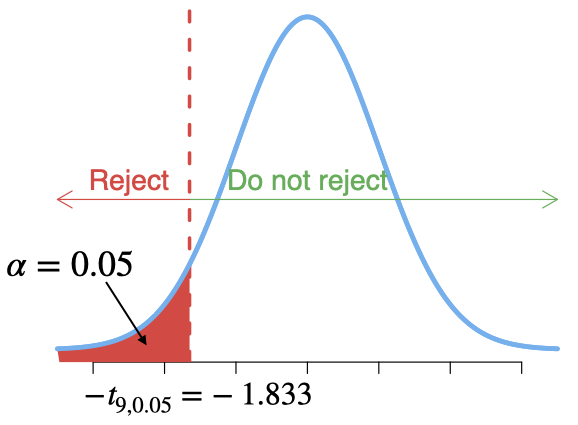
\includegraphics[width=0.35\linewidth,height=0.35\textheight]{figures/correx1} \end{center}

\textbf{Using R:}

First we need to enter the data in R.

\begin{Shaded}
\begin{Highlighting}[]
\NormalTok{Price}\OtherTok{\textless{}{-}}\FunctionTok{c}\NormalTok{(}\DecValTok{85}\NormalTok{, }\DecValTok{103}\NormalTok{,  }\DecValTok{70}\NormalTok{,  }\DecValTok{82}\NormalTok{,  }\DecValTok{89}\NormalTok{,  }\DecValTok{98}\NormalTok{,  }\DecValTok{66}\NormalTok{,  }\DecValTok{95}\NormalTok{, }\DecValTok{169}\NormalTok{,  }\DecValTok{70}\NormalTok{,  }\DecValTok{48}\NormalTok{)}
\NormalTok{Age}\OtherTok{\textless{}{-}} \FunctionTok{c}\NormalTok{(}\DecValTok{5}\NormalTok{, }\DecValTok{4}\NormalTok{, }\DecValTok{6}\NormalTok{, }\DecValTok{5}\NormalTok{, }\DecValTok{5}\NormalTok{, }\DecValTok{5}\NormalTok{, }\DecValTok{6}\NormalTok{, }\DecValTok{6}\NormalTok{, }\DecValTok{2}\NormalTok{, }\DecValTok{7}\NormalTok{, }\DecValTok{7}\NormalTok{)}
\NormalTok{carSales}\OtherTok{\textless{}{-}}\FunctionTok{data.frame}\NormalTok{(Price,Age)}
\FunctionTok{str}\NormalTok{(carSales)}
\end{Highlighting}
\end{Shaded}

\begin{verbatim}
## 'data.frame':    11 obs. of  2 variables:
##  $ Price: num  85 103 70 82 89 98 66 95 169 70 ...
##  $ Age  : num  5 4 6 5 5 5 6 6 2 7 ...
\end{verbatim}

Now let us plot \texttt{age} against \texttt{price}, i.e.~a scatterplot.

\begin{Shaded}
\begin{Highlighting}[]
\FunctionTok{plot}\NormalTok{(Price }\SpecialCharTok{\textasciitilde{}}\NormalTok{ Age, }\AttributeTok{pch=}\DecValTok{16}\NormalTok{, }\AttributeTok{col=}\DecValTok{2}\NormalTok{)}
\end{Highlighting}
\end{Shaded}

\begin{center}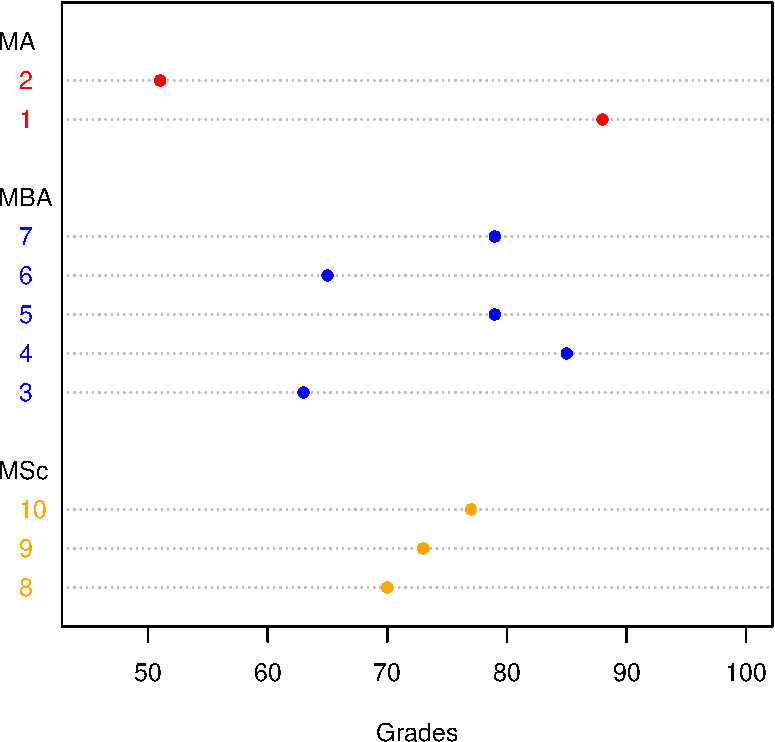
\includegraphics[width=0.5\linewidth,height=0.5\textheight]{unnamed-chunk-26-1} \end{center}

or we can use ggplot2 for a much nicer plot.

\begin{Shaded}
\begin{Highlighting}[]
\FunctionTok{library}\NormalTok{(ggplot2)}
\CommentTok{\# Basic scatter plot}
\FunctionTok{ggplot}\NormalTok{(carSales, }\FunctionTok{aes}\NormalTok{(}\AttributeTok{x=}\NormalTok{Age, }\AttributeTok{y=}\NormalTok{Price)) }\SpecialCharTok{+} \FunctionTok{geom\_point}\NormalTok{()}
\end{Highlighting}
\end{Shaded}

\begin{center}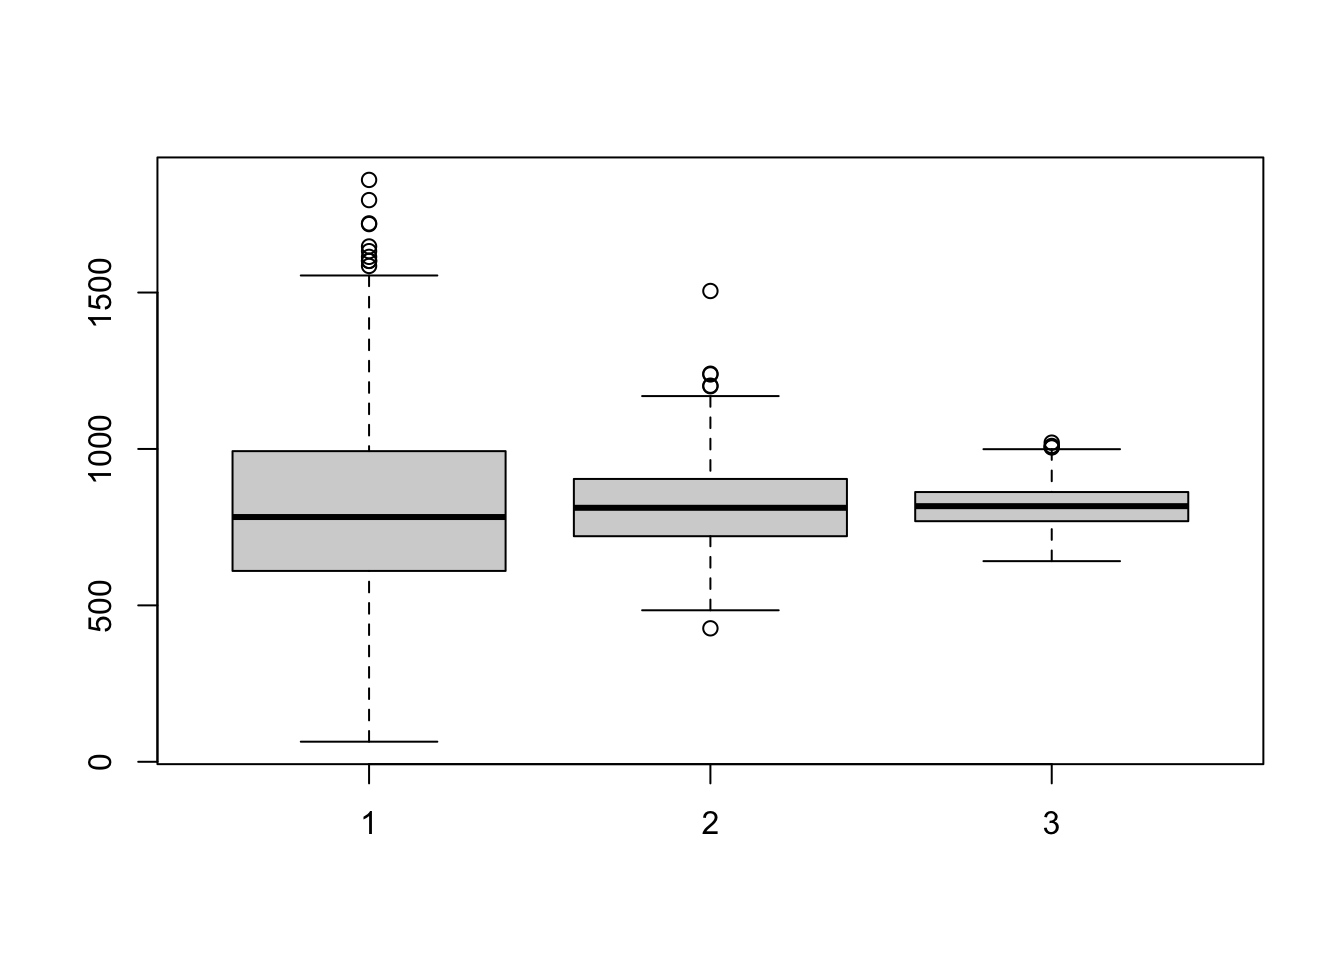
\includegraphics[width=0.5\linewidth,height=0.5\textheight]{unnamed-chunk-27-1} \end{center}

From this plot it seems that there is a negative linear relationship
between age and price. There are several tools that can help us to
measure this relationship more precisely.

\begin{Shaded}
\begin{Highlighting}[]
\FunctionTok{cor.test}\NormalTok{(Age, Price,}
         \AttributeTok{alternative =} \StringTok{"less"}\NormalTok{,}
         \AttributeTok{method =} \StringTok{"pearson"}\NormalTok{, }\AttributeTok{conf.level =} \FloatTok{0.95}\NormalTok{)}
\end{Highlighting}
\end{Shaded}

\begin{verbatim}
## 
##  Pearson's product-moment correlation
## 
## data:  Age and Price
## t = -7.2374, df = 9, p-value = 2.441e-05
## alternative hypothesis: true correlation is less than 0
## 95 percent confidence interval:
##  -1.0000000 -0.7749819
## sample estimates:
##        cor 
## -0.9237821
\end{verbatim}

Suppose now we scale both variables (standardized)

\begin{Shaded}
\begin{Highlighting}[]
\FunctionTok{cor.test}\NormalTok{(}\FunctionTok{scale}\NormalTok{(Age), }\FunctionTok{scale}\NormalTok{(Price),}
         \AttributeTok{alternative =} \StringTok{"less"}\NormalTok{,}
         \AttributeTok{method =} \StringTok{"pearson"}\NormalTok{, }\AttributeTok{conf.level =} \FloatTok{0.95}\NormalTok{)}
\end{Highlighting}
\end{Shaded}

\begin{verbatim}
## 
##  Pearson's product-moment correlation
## 
## data:  scale(Age) and scale(Price)
## t = -7.2374, df = 9, p-value = 2.441e-05
## alternative hypothesis: true correlation is less than 0
## 95 percent confidence interval:
##  -1.0000000 -0.7749819
## sample estimates:
##        cor 
## -0.9237821
\end{verbatim}

We notice that corr(age, price in pounds) \(=\) corr(age, price in
dollars).

\(~\)

We can also obtain Spearman's rho and Kendall's tau as follows.

\begin{Shaded}
\begin{Highlighting}[]
\FunctionTok{cor.test}\NormalTok{(Age, Price,}
         \AttributeTok{alternative =} \StringTok{"less"}\NormalTok{,}
         \AttributeTok{method =} \StringTok{"spearman"}\NormalTok{, }\AttributeTok{conf.level =} \FloatTok{0.95}\NormalTok{)}
\end{Highlighting}
\end{Shaded}

\begin{verbatim}
## 
##  Spearman's rank correlation rho
## 
## data:  Age and Price
## S = 403.26, p-value = 0.0007267
## alternative hypothesis: true rho is less than 0
## sample estimates:
##        rho 
## -0.8330014
\end{verbatim}

\begin{Shaded}
\begin{Highlighting}[]
\FunctionTok{cor.test}\NormalTok{(Age, Price,}
         \AttributeTok{alternative =} \StringTok{"less"}\NormalTok{,}
         \AttributeTok{method =} \StringTok{"kendall"}\NormalTok{, }\AttributeTok{conf.level =} \FloatTok{0.95}\NormalTok{)}
\end{Highlighting}
\end{Shaded}

\begin{verbatim}
## 
##  Kendall's rank correlation tau
## 
## data:  Age and Price
## z = -2.9311, p-value = 0.001689
## alternative hypothesis: true tau is less than 0
## sample estimates:
##        tau 
## -0.7302967
\end{verbatim}

\(~\)

As the p-values for all three tests (Pearson, Spearman, Kendall) less
than \(\alpha=0.05\), we reject the null hypothesis of no correlation
between the age and the price, at the 5\% significance level.

\(~\)

\textbf{Now what do you think about correlation and causation?}

\begin{figure}

{\centering 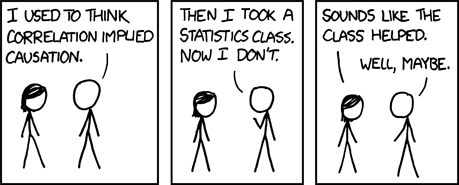
\includegraphics[width=0.6\linewidth,height=0.6\textheight]{figures/correlationxkcd} 

}

\caption{https://xkcd.com/552/}\label{fig:unnamed-chunk-31}
\end{figure}

\hypertarget{simple-regression-introduction-1}{%
\section{Simple regression:
Introduction}\label{simple-regression-introduction-1}}

\hypertarget{motivation-1}{%
\subsection{Motivation}\label{motivation-1}}

\textbf{Predicting the Price of a used car}

\begin{center}
\includegraphics[width=0.6\linewidth,height=0.6\textheight]{figures/motivation1} \end{center}

\begin{center}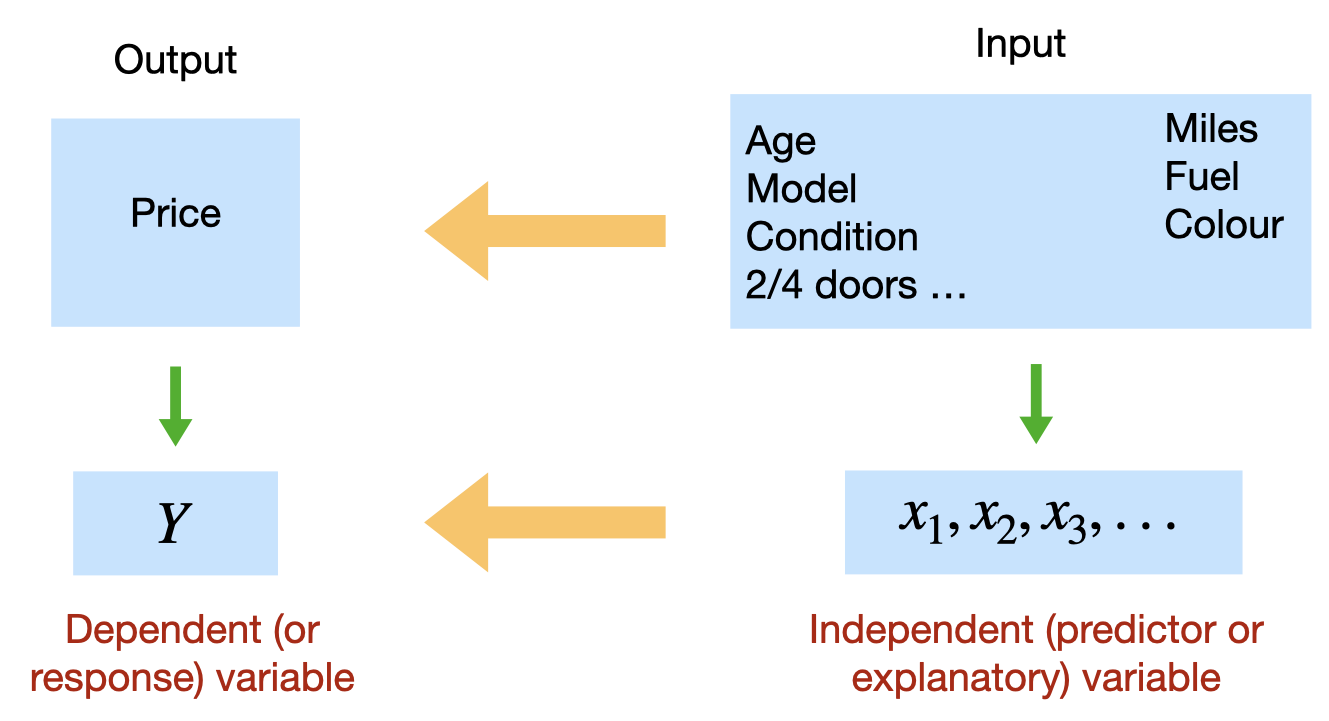
\includegraphics[width=0.6\linewidth,height=0.6\textheight]{figures/motivation2} \end{center}

\hypertarget{simple-linear-regression-1}{%
\subsection{Simple linear regression}\label{simple-linear-regression-1}}

\textbf{Simple linear regression (population)}
\[Y=\beta_0+\beta_1 x+\epsilon\] In our example:
\[Price=\beta_0+\beta_1 Age+\epsilon\]

\textbf{Simple linear regression (sample)} \[\hat{y}=b_0+b_1 x\] where
the coefficient \(\beta_0\) (and its estimate \(b_0\) or
\(\hat{\beta}_0\) ) refers to the \(y\)-intercept or simply the
intercept or the constant of the regression line, and the coefficient
\(\beta_1\) (and its estimate \(b_1\) or \(\hat{\beta}_1\) ) refers to
the slope of the regression line.

\hypertarget{least-squares-criterion-1}{%
\subsection{Least-Squares criterion}\label{least-squares-criterion-1}}

\begin{itemize}
\item
  The \textbf{least-squares criterion} is that the line that best fits a
  set of data points is the one having the smallest possible sum of
  squared errors. The `errors' are the vertical distances of the data
  points to the line.
\item
  We need to use the data to estimate the values of the parameters
  \(\beta_0\) and \(\beta_1\), i.e.~to fit a straight line to the set of
  points \(\{(x_i , y_i )\}\). There are many straight lines we could
  use, so we need some idea of which is best. Clearly, a bad straight
  line model would be one that had many large errors, and conversely, a
  good straight line model will have, on average, small errors. We
  quantify this by the sum of squares of the errors:
  \[Q(\beta_0,\beta_1)=\sum_{i=1}^n \epsilon_i^2=\sum_{i=1}^n[y_i-(\beta_0 + \beta_1 x_i)]^2\]
  then the ``line of best fit'' will correspond to the line with values
  of \(\beta_0\) and \(\beta_1\) that minimises \(Q(\beta_0,\beta_1)\).
\item
  The regression line is the line that fits a set of data points
  according to the least squares criterion.
\item
  The regression equation is the equation of the regression line.
\item
  The regression equation for a set of \(n\) data points is
  \(\hat{y}=b_0+b_1\;x\), where
  \[b_1=\frac{S_{xy}}{S_{xx}}=\frac{\sum (x_i-\bar{x})(y_i-\bar{y})}{\sum (x_i-\bar{x})^2}
   \;\;\text{and}\;\; b_0=\bar{y}-b_1\; \bar{x}\]
\item
  \(y\) is the dependent variable (or response variable) and \(x\) is
  the independent variable (predictor variable or explanatory variable).
\item
  \(b_0\) is called the \textbf{y-intercept} and \(b_1\) is called the
  \textbf{slope}.
\end{itemize}

\begin{center}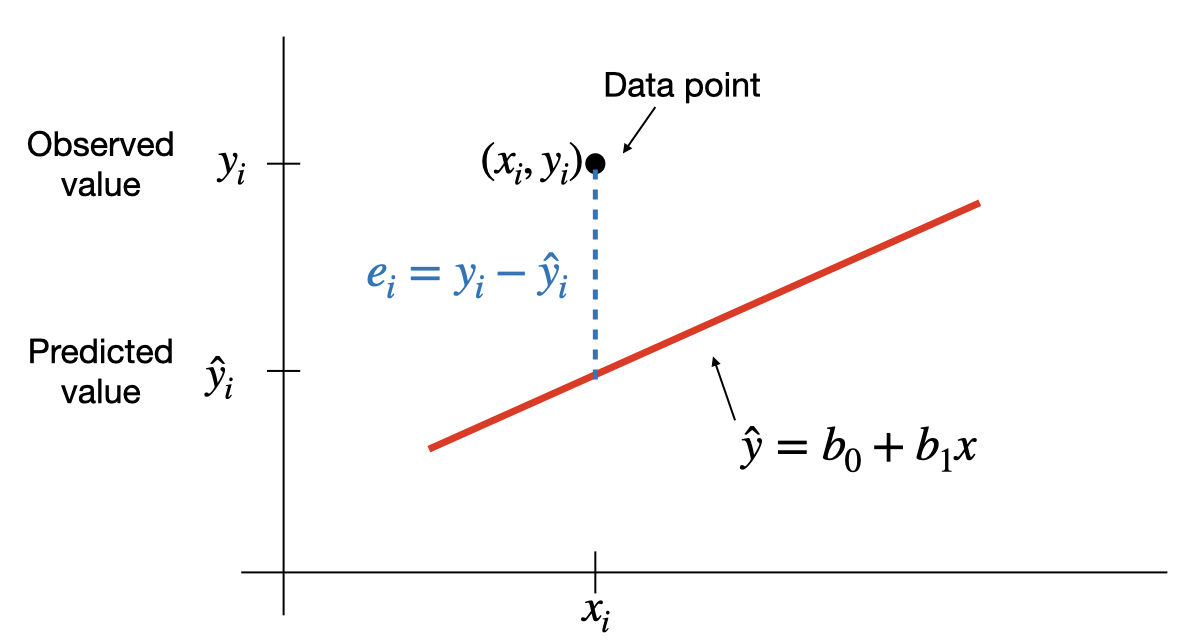
\includegraphics[width=0.6\linewidth,height=0.6\textheight]{figures/leastsq2} \end{center}

\textbf{SSE and the standard error}

This least square regression line minimizes the error sum of squares
\[SSE=\sum e^2_i =\sum (y_i-\hat{y}_i)^2\] The standard error of the
estimate, \(s_e=\sqrt{SSE/(n-2)}\), indicates how much, on average, the
observed values of the response variable differ from the predicated
values of the response variable.

\begin{center}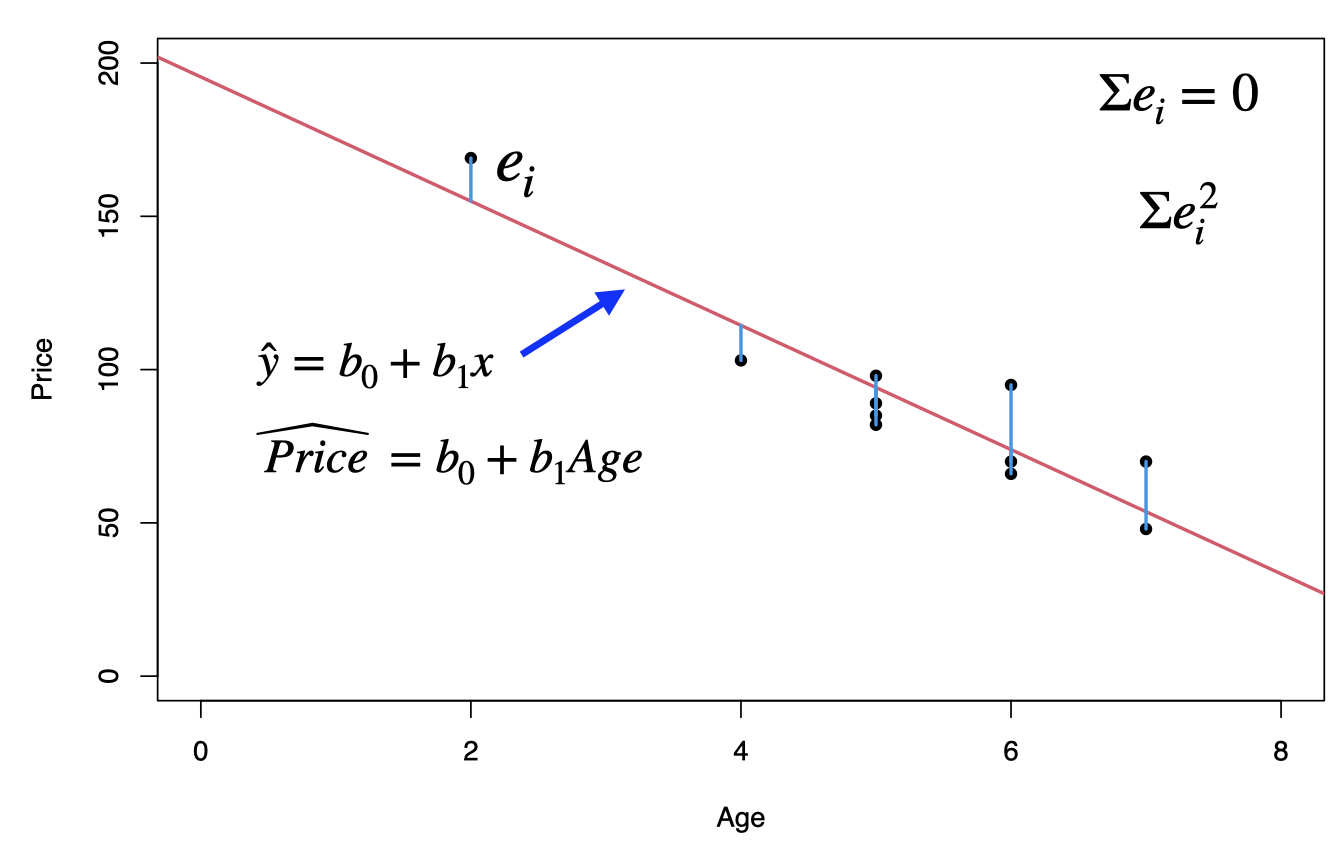
\includegraphics[width=0.6\linewidth,height=0.6\textheight]{figures/leastsq1} \end{center}

\hypertarget{example-used-cars-cont.-1}{%
\subsection{Example: used cars
(cont.)}\label{example-used-cars-cont.-1}}

The table below displays data on Age (in years) and Price (in hundreds
of dollars) for a sample of cars of a particular make and model.(Weiss,
2012)

\begin{longtable}[]{@{}cc@{}}
\toprule\noalign{}
Price (\(y\)) & Age (\(x\)) \\
\midrule\noalign{}
\endhead
\bottomrule\noalign{}
\endlastfoot
85 & 5 \\
103 & 4 \\
70 & 6 \\
82 & 5 \\
89 & 5 \\
98 & 5 \\
66 & 6 \\
95 & 6 \\
169 & 2 \\
70 & 7 \\
48 & 7 \\
\end{longtable}

\begin{itemize}
\item
  For our example, \emph{age} is the predictor variable and \emph{price}
  is the response variable.
\item
  The regression equation is \(\hat{y}=195.47-20.26\;x\), where the
  slope \(b_1=-20.26\) and the intercept \(b_0=195.47\)
\item
  Prediction: for \(x = 4\), that is we would like to predict the price
  of a 4-year-old car,
  \[\hat{y}=195.47-20.26 {\color{blue}(4)}= 114.43 \;\;\text{or}\;\; \$ 11443\]
\end{itemize}

\begin{center}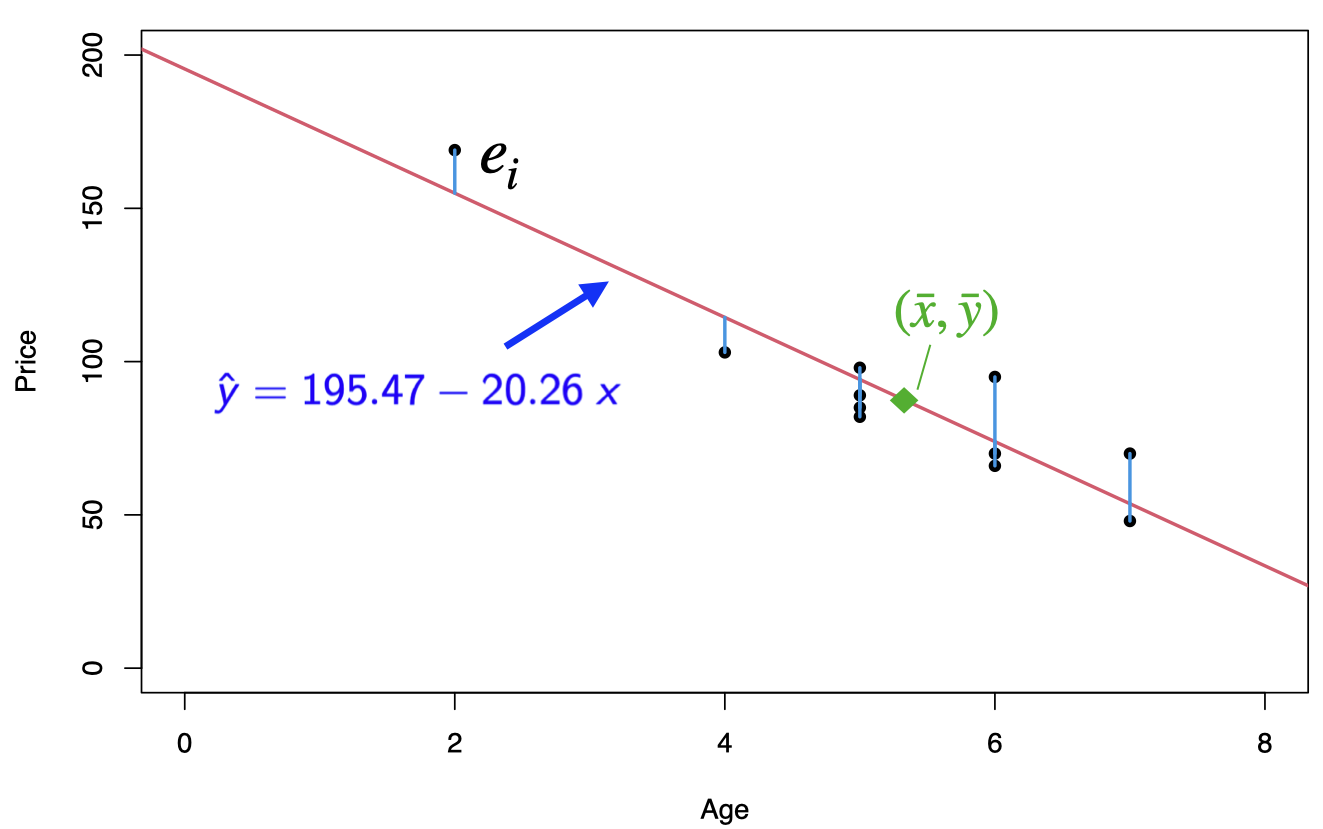
\includegraphics[width=0.6\linewidth,height=0.6\textheight]{figures/leastsq5} \end{center}

Back to our used cars example, we want to find the ``best line'' through
the data points, which can be used to predict prices of used cars based
on their age.

First we need to enter the data in R.

\begin{Shaded}
\begin{Highlighting}[]
\NormalTok{Price}\OtherTok{\textless{}{-}}\FunctionTok{c}\NormalTok{(}\DecValTok{85}\NormalTok{, }\DecValTok{103}\NormalTok{,  }\DecValTok{70}\NormalTok{,  }\DecValTok{82}\NormalTok{,  }\DecValTok{89}\NormalTok{,  }\DecValTok{98}\NormalTok{,  }\DecValTok{66}\NormalTok{,  }\DecValTok{95}\NormalTok{, }\DecValTok{169}\NormalTok{,  }\DecValTok{70}\NormalTok{,  }\DecValTok{48}\NormalTok{)}
\NormalTok{Age}\OtherTok{\textless{}{-}} \FunctionTok{c}\NormalTok{(}\DecValTok{5}\NormalTok{, }\DecValTok{4}\NormalTok{, }\DecValTok{6}\NormalTok{, }\DecValTok{5}\NormalTok{, }\DecValTok{5}\NormalTok{, }\DecValTok{5}\NormalTok{, }\DecValTok{6}\NormalTok{, }\DecValTok{6}\NormalTok{, }\DecValTok{2}\NormalTok{, }\DecValTok{7}\NormalTok{, }\DecValTok{7}\NormalTok{)}
\NormalTok{carSales}\OtherTok{\textless{}{-}}\FunctionTok{data.frame}\NormalTok{(Price,Age)}
\FunctionTok{str}\NormalTok{(carSales)}
\end{Highlighting}
\end{Shaded}

\begin{verbatim}
## 'data.frame':    11 obs. of  2 variables:
##  $ Price: num  85 103 70 82 89 98 66 95 169 70 ...
##  $ Age  : num  5 4 6 5 5 5 6 6 2 7 ...
\end{verbatim}

\begin{Shaded}
\begin{Highlighting}[]
\FunctionTok{cor}\NormalTok{(Age, Price, }\AttributeTok{method =} \StringTok{"pearson"}\NormalTok{)}
\end{Highlighting}
\end{Shaded}

\begin{verbatim}
## [1] -0.9237821
\end{verbatim}

Scatterplot: Age vs.~Price

\begin{Shaded}
\begin{Highlighting}[]
\FunctionTok{library}\NormalTok{(ggplot2)}
\FunctionTok{ggplot}\NormalTok{(carSales, }\FunctionTok{aes}\NormalTok{(}\AttributeTok{x=}\NormalTok{Age, }\AttributeTok{y=}\NormalTok{Price)) }\SpecialCharTok{+} \FunctionTok{geom\_point}\NormalTok{()}
\end{Highlighting}
\end{Shaded}

\begin{center}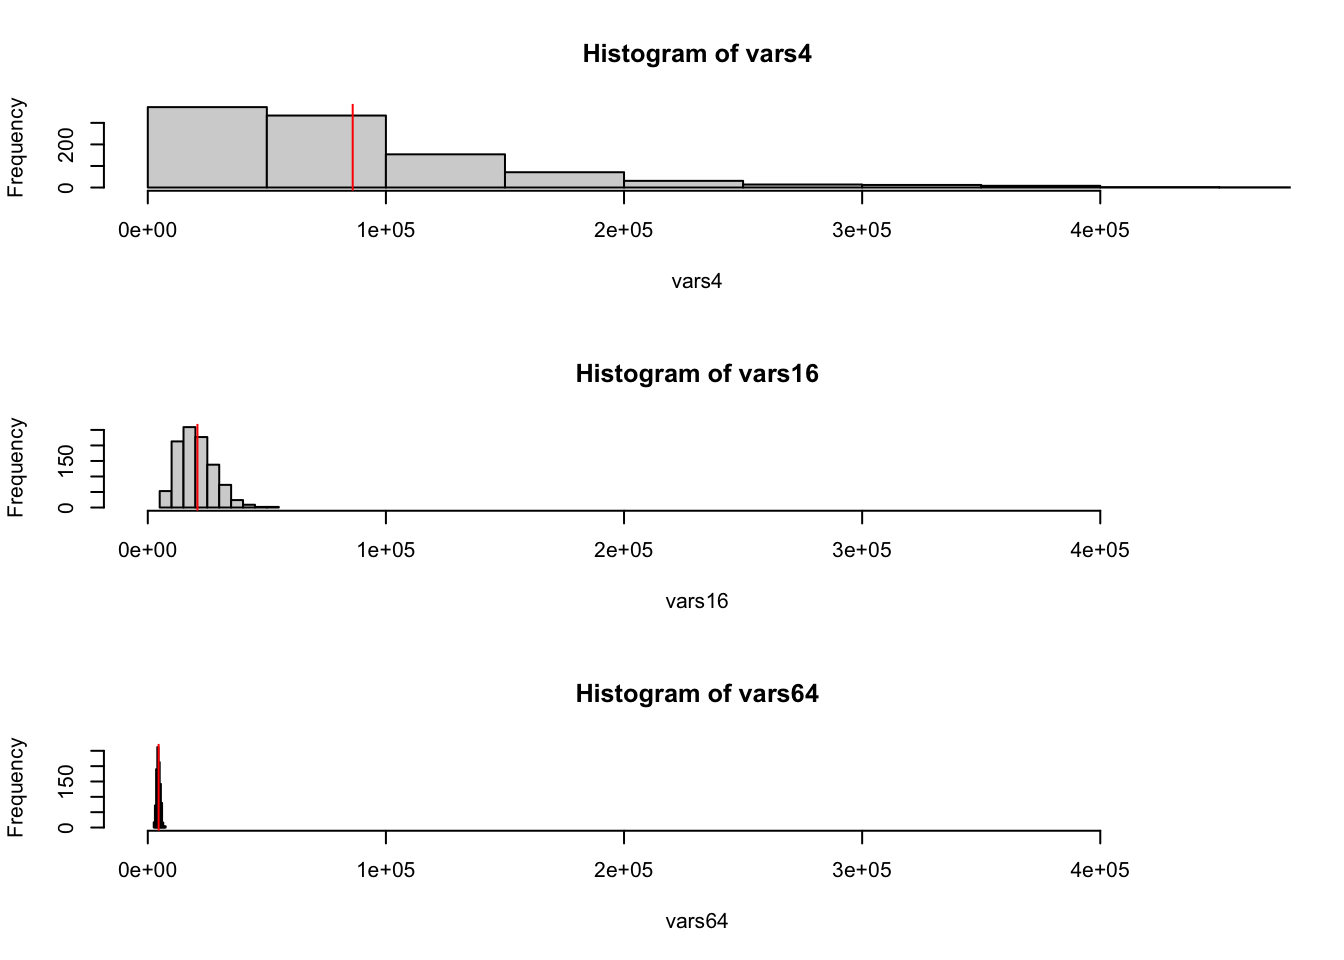
\includegraphics[width=0.5\linewidth,height=0.5\textheight]{unnamed-chunk-38-1} \end{center}

\begin{Shaded}
\begin{Highlighting}[]
\CommentTok{\# Remove the confidence interval}
\FunctionTok{ggplot}\NormalTok{(carSales, }\FunctionTok{aes}\NormalTok{(}\AttributeTok{x=}\NormalTok{Age, }\AttributeTok{y=}\NormalTok{Price)) }\SpecialCharTok{+} 
  \FunctionTok{geom\_point}\NormalTok{()}\SpecialCharTok{+}
  \FunctionTok{geom\_smooth}\NormalTok{(}\AttributeTok{method=}\NormalTok{lm, }\AttributeTok{formula=}\NormalTok{ y}\SpecialCharTok{\textasciitilde{}}\NormalTok{x, }\AttributeTok{se=}\ConstantTok{FALSE}\NormalTok{)}
\end{Highlighting}
\end{Shaded}

%\begin{center}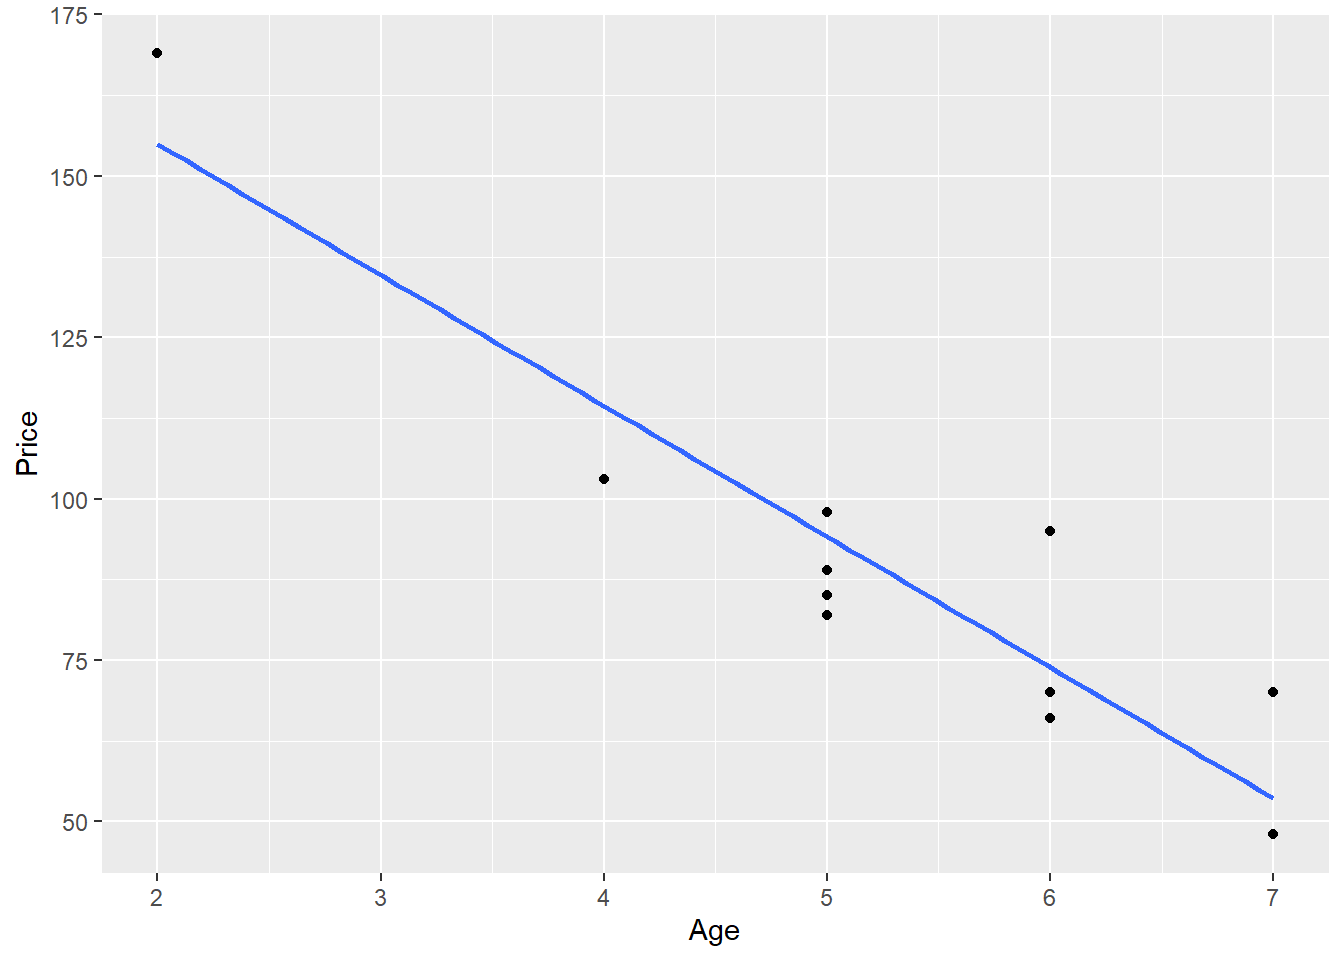
\includegraphics[width=0.5\linewidth,height=0.5\textheight]{unnamed-chunk-39-1} \end{center}

\hypertarget{prediction-1}{%
\subsection{Prediction}\label{prediction-1}}

\begin{Shaded}
\begin{Highlighting}[]
\CommentTok{\# simple linear regression}
\NormalTok{reg}\OtherTok{\textless{}{-}}\FunctionTok{lm}\NormalTok{(Price}\SpecialCharTok{\textasciitilde{}}\NormalTok{Age)}
\FunctionTok{print}\NormalTok{(reg)}
\end{Highlighting}
\end{Shaded}

\begin{verbatim}
## 
## Call:
## lm(formula = Price ~ Age)
## 
## Coefficients:
## (Intercept)          Age  
##      195.47       -20.26
\end{verbatim}

To predict the price of a 4-year-old car (\(x=4\)):
\[\hat{y}=195.47-20.26(4)=114.43\]

\begin{center}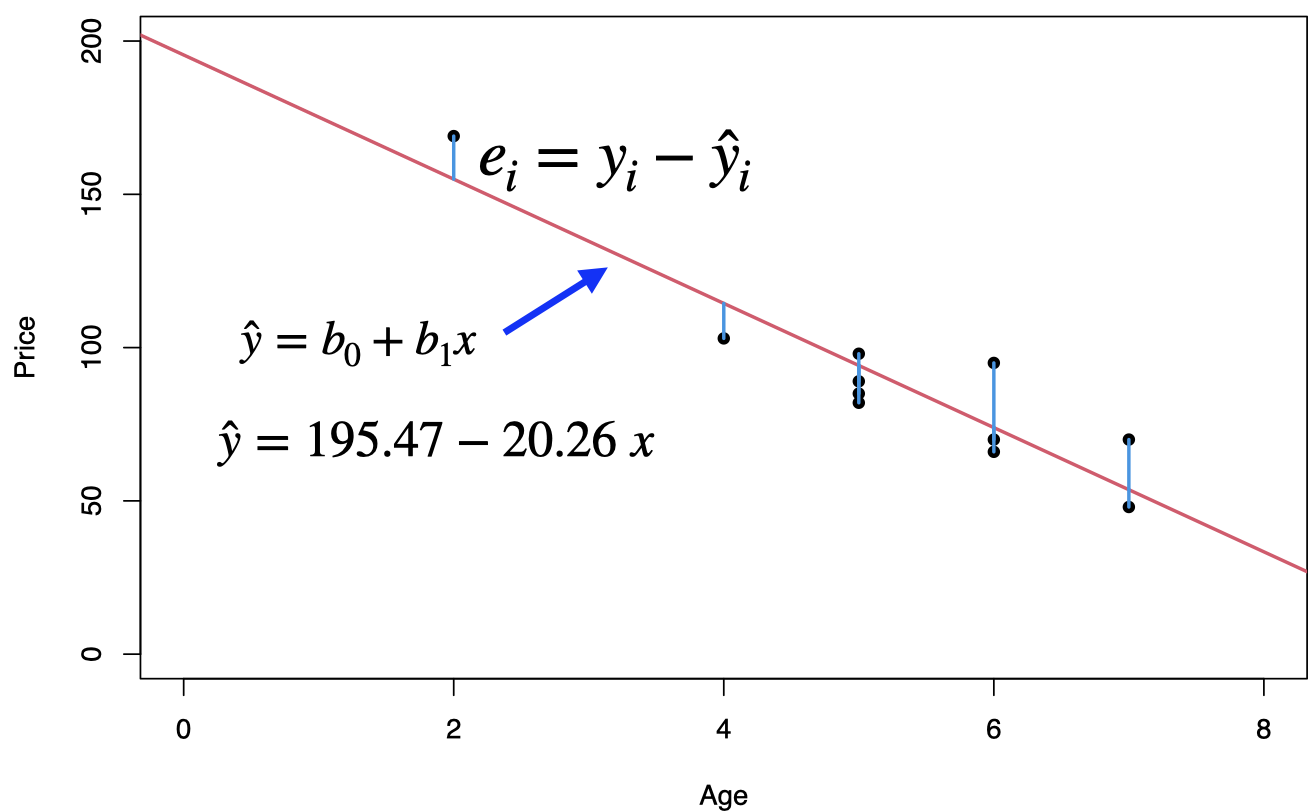
\includegraphics[width=0.6\linewidth,height=0.6\textheight]{figures/leastsq3} \end{center}

\hypertarget{simple-regression-coefficient-of-determination-1}{%
\section{Simple Regression: Coefficient of
Determination}\label{simple-regression-coefficient-of-determination-1}}

\hypertarget{extrapolation-1}{%
\subsection{Extrapolation}\label{extrapolation-1}}

\begin{itemize}
\item
  Within the range of the observed values of the predictor variable, we
  can reasonably use the regression equation to make predictions for the
  response variable.
\item
  However, to do so outside the range, which is called
  \textbf{Extrapolation}, may not be reasonable because the linear
  relationship between the predictor and response variables may not hold
  here.
\item
  To predict the price of an 11-year old car,
  \(\hat{y}=195.47-20.26 (11)=-27.39\) or \$ 2739, this result is
  unrealistic as no one is going to pay us \$2739 to take away their
  11-year old car.
\end{itemize}

\begin{center}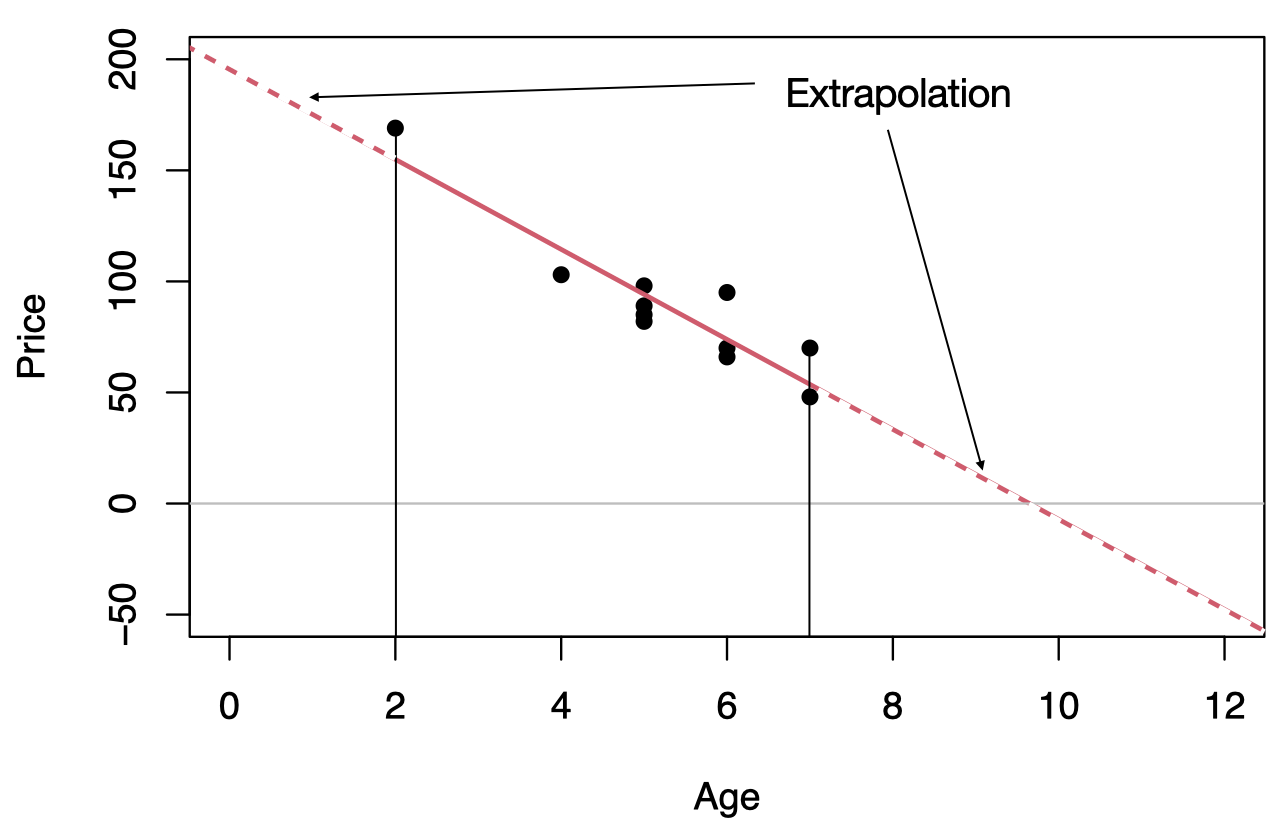
\includegraphics[width=0.6\linewidth,height=0.6\textheight]{figures/extrap} \end{center}

\hypertarget{outliers-and-influential-observations-1}{%
\subsection{Outliers and influential
observations}\label{outliers-and-influential-observations-1}}

\begin{itemize}
\item
  Recall that an \textbf{outlier} is an observation that lies outside
  the overall pattern of the data. In the context of regression, an
  outlier is a data point that lies far from the regression line,
  relative to the other data points.
\item
  An \textbf{influential observation} is a data point whose removal
  causes the regression equation (and line) to change considerably.
\item
  From the scatterplot, it seems that the data point (2,169) might be an
  influential observation. Removing that data point and recalculating
  the regression equation yields \(\hat{y}=160.33-14.24\;x\).
\end{itemize}

\begin{center}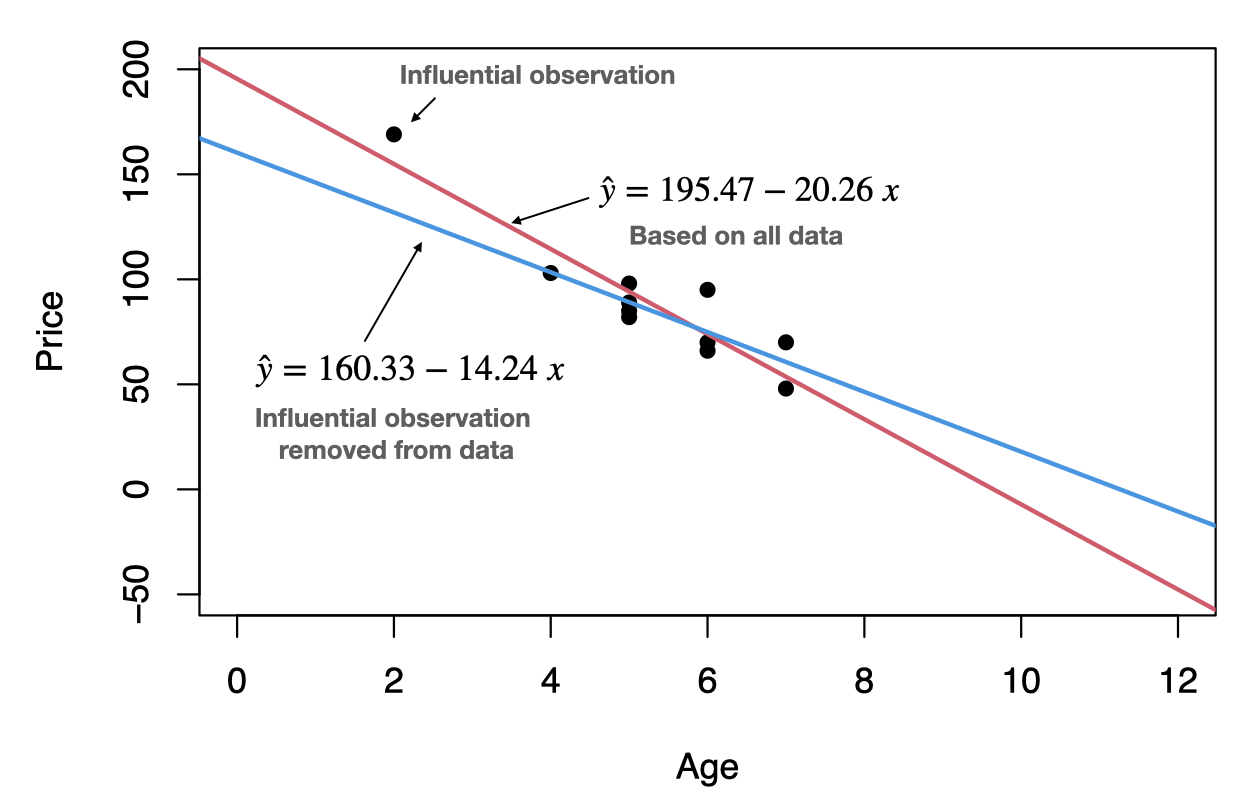
\includegraphics[width=0.6\linewidth,height=0.6\textheight]{figures/outliersreg} \end{center}

\hypertarget{coefficient-of-determination-1}{%
\subsection{Coefficient of
determination}\label{coefficient-of-determination-1}}

\begin{center}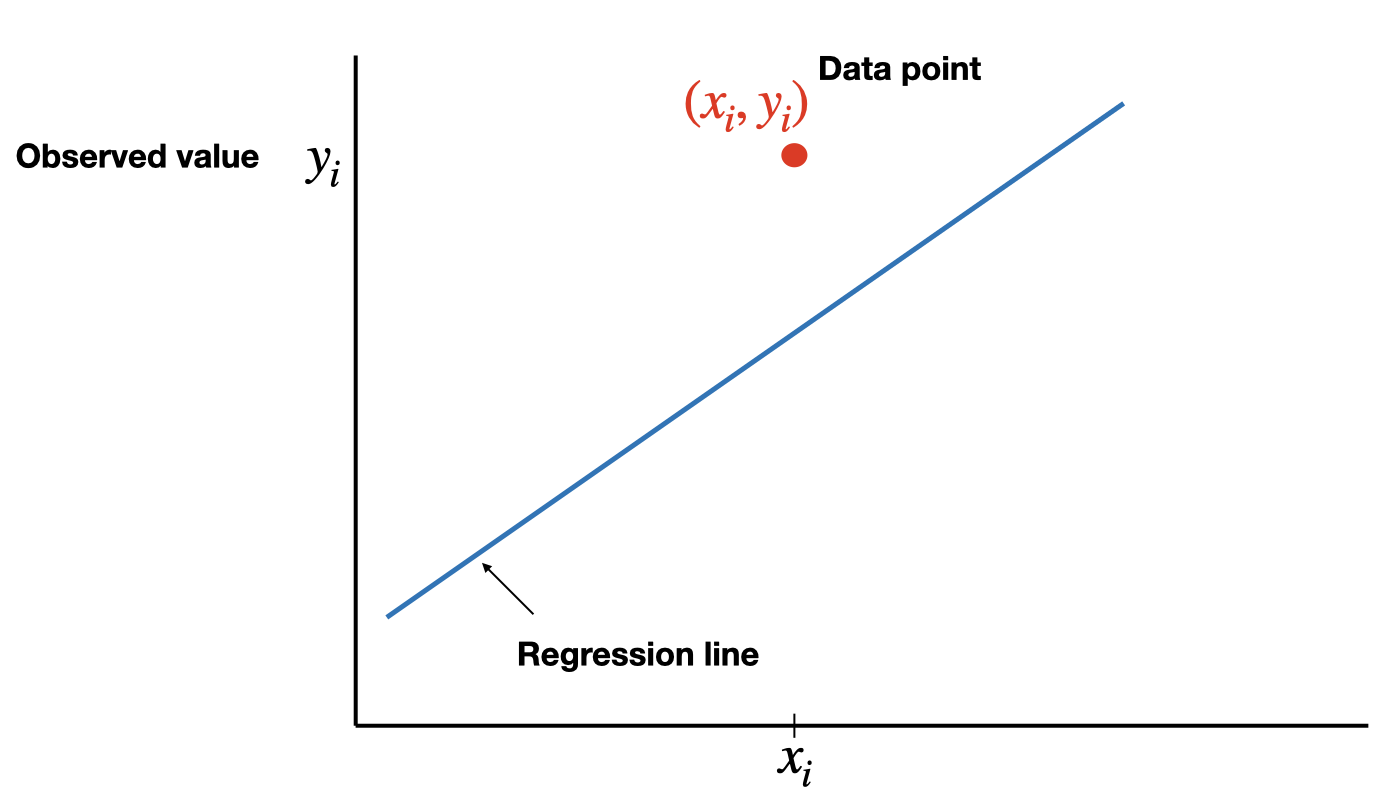
\includegraphics[width=0.6\linewidth,height=0.6\textheight]{figures/cod1} \end{center}

\begin{center}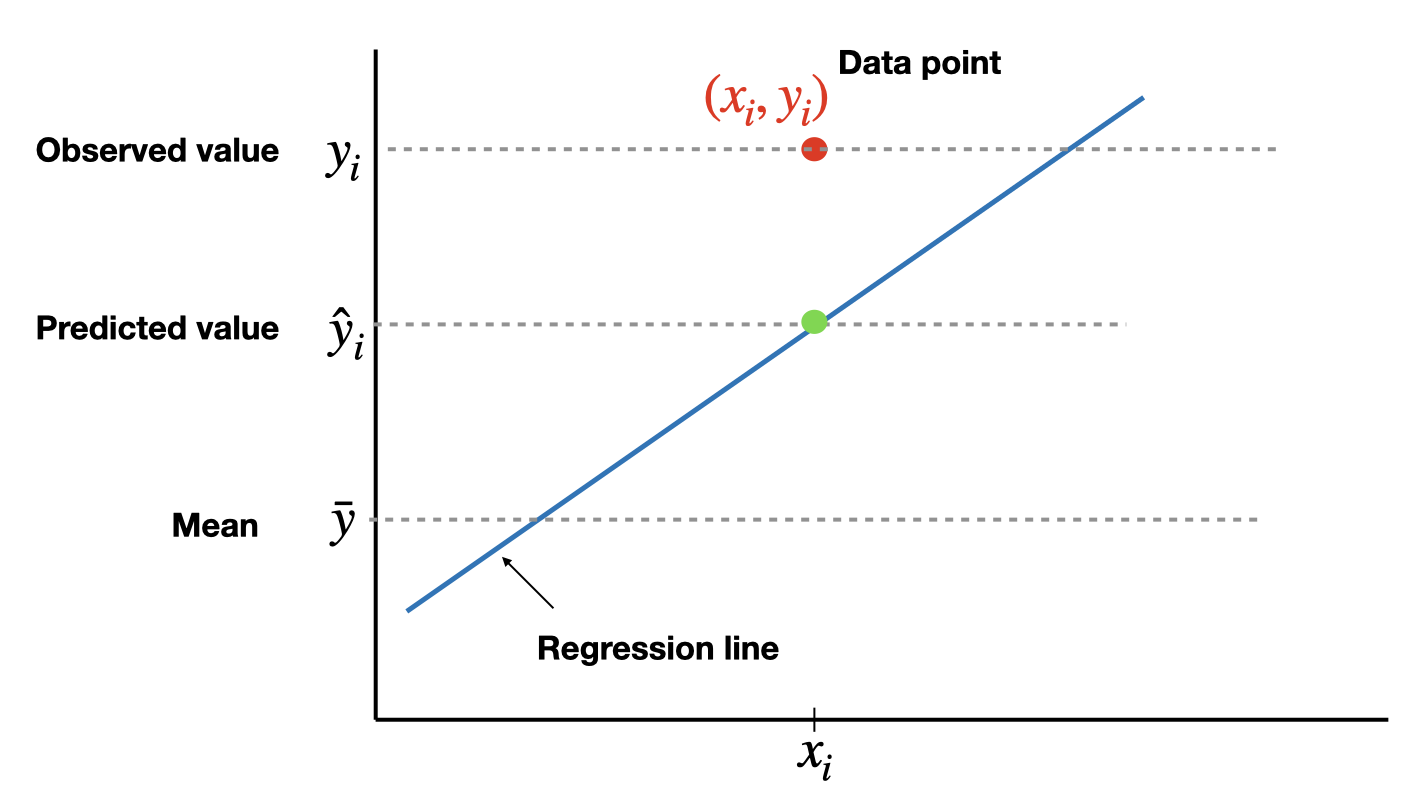
\includegraphics[width=0.6\linewidth,height=0.6\textheight]{figures/cod2} \end{center}

\begin{center}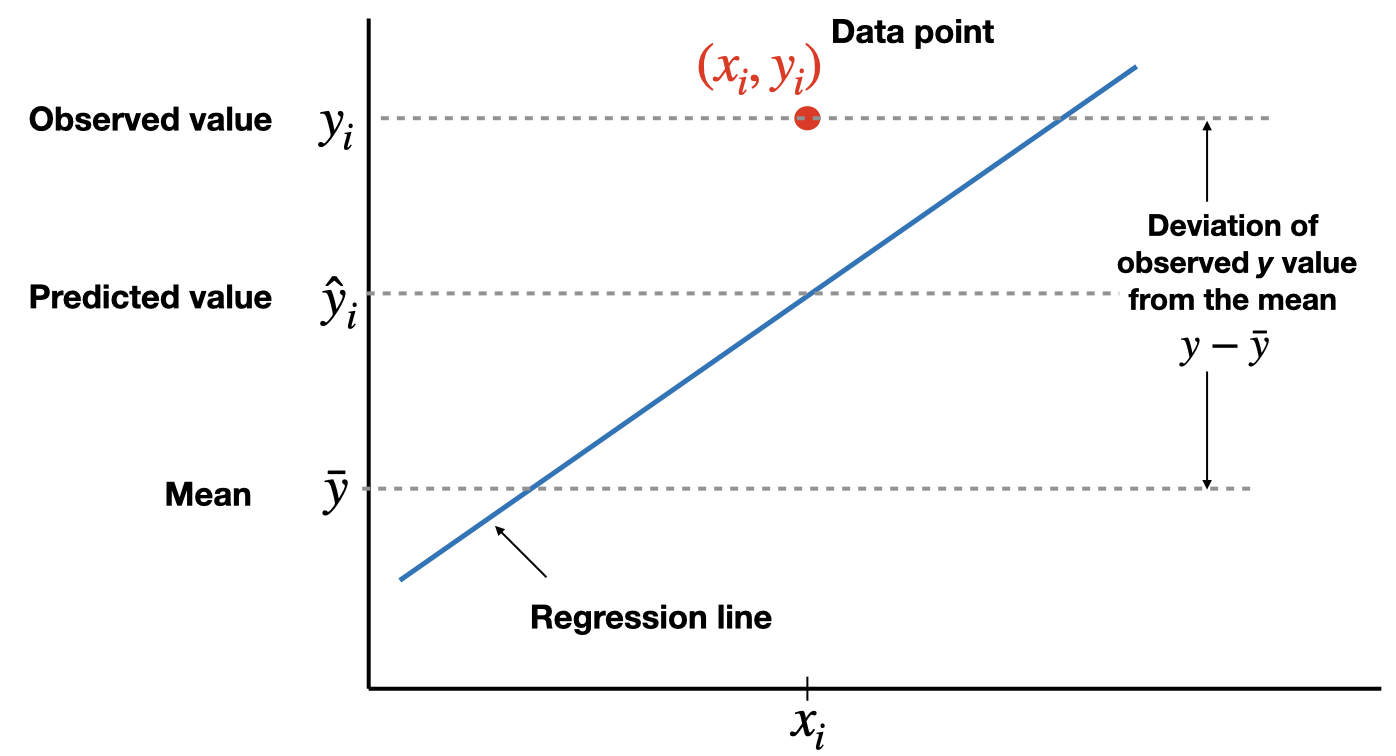
\includegraphics[width=0.6\linewidth,height=0.6\textheight]{figures/cod3} \end{center}

\begin{center}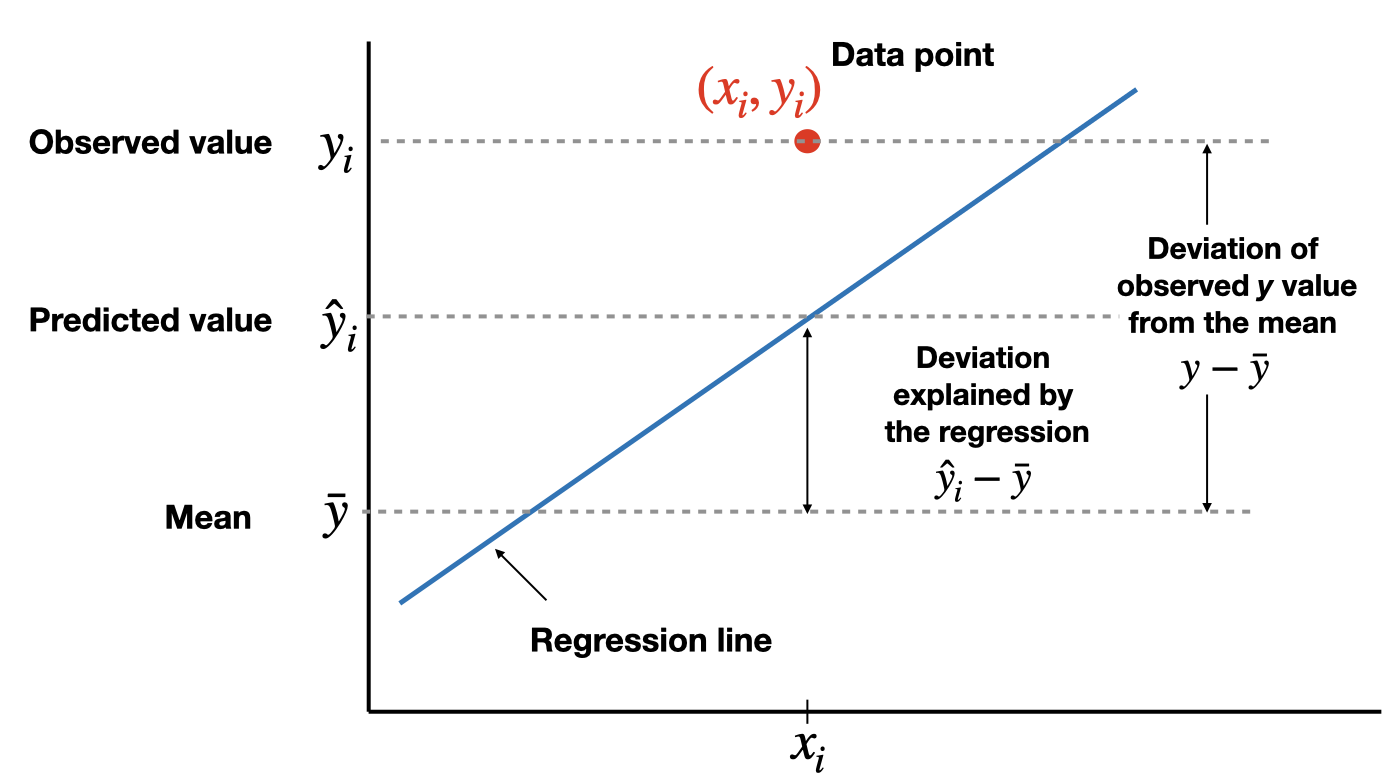
\includegraphics[width=0.6\linewidth,height=0.6\textheight]{figures/cod4} \end{center}

\begin{center}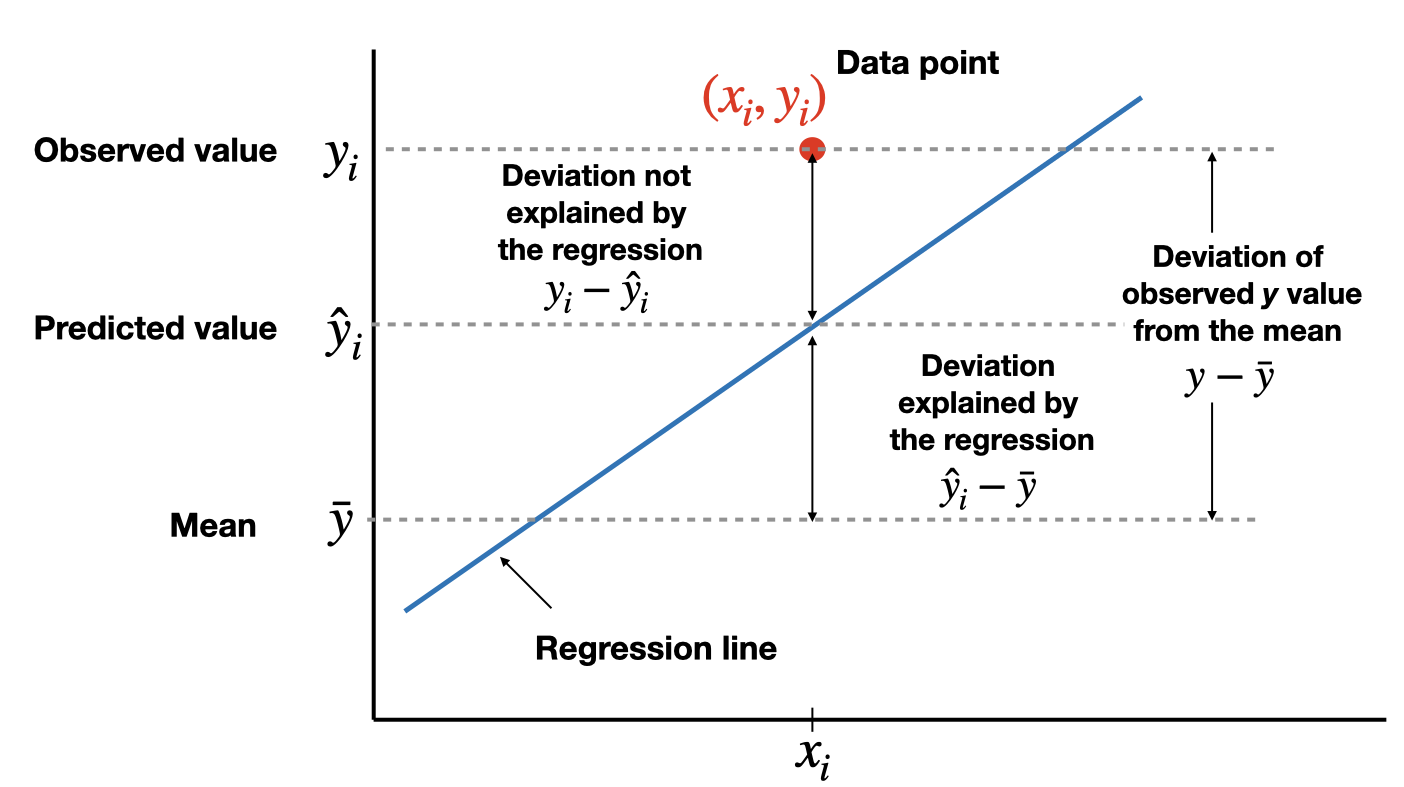
\includegraphics[width=0.6\linewidth,height=0.6\textheight]{figures/cod5} \end{center}

\begin{itemize}
\item
  The total variation in the observed values of the response variable,
  \(SST=\sum(y_i-\bar{y})^2\), can be partitioned into two components:

  \begin{itemize}
  \tightlist
  \item
    The variation in the observed values of the response variable
    explained by the regression: \(SSR=\sum(\hat{y}_i-\bar{y})^2\)
  \item
    The variation in the observed values of the response variable not
    explained by the regression: \(SSE=\sum(y_i-\hat{y}_i)^2\)
  \end{itemize}
\item
  The coefficient of determination, \(R^2\) (or \(R\)-square), is the
  proportion of the variation in the observed values of the response
  variable explained by the regression, which is given by
  \[R^2=\frac{SSR}{SST}=\frac{SST-SSE}{SST}=1-\frac{SSE}{SST}\] where
  \(SST=SSR+SSE\). \(R^2\) is a descriptive measure of the utility of
  the regression equation for making prediction.
\item
  The coefficient of determination \(R^2\) always lies between 0 and 1.
  A value of \(R^2\) near 0 suggests that the regression equation is not
  very useful for making predictions, whereas a value of \(R^2\) near 1
  suggests that the regression equation is quite useful for making
  predictions.
\item
  For a simple linear regression (one independent variable) ONLY,
  \(R^2\) is the square of Pearson correlation coefficient, \(r\).
\item
  \(\text{Adjusted}\;R^2\) is a modification of \(R^2\) which takes into
  account the number of independent variables, say \(k\). In a simple
  linear regression \(k=1\). Adjusted-\(R^2\) increases only when a
  significant related independent variable is added to the model.
  Adjusted-\(R^2\) has a crucial role in the process of model building.
  Adjusted-\(R^2\) is given by
  \[\text{Adjusted-}R^2=1-(1-R^2)\frac{n-1}{n-k-1}\]
\end{itemize}

\hypertarget{notation-used-in-regression-1}{%
\subsection{Notation used in
regression}\label{notation-used-in-regression-1}}

\begin{longtable}[]{@{}ccl@{}}
\toprule\noalign{}
Quantity & Defining formula & Computing formula \\
\midrule\noalign{}
\endhead
\bottomrule\noalign{}
\endlastfoot
\(S_{xx}\) & \(\sum (x_i-\bar{x})^2\) & \(\sum x^2_i - n \bar{x}^2\) \\
\(S_{xy}\) & \(\sum (x_i-\bar{x})(y_i-\bar{y})\) &
\(\sum x_i y_i - n \bar{x}\bar{y}\) \\
\(S_{yy}\) & \(\sum (y_i-\bar{y})^2\) & \(\sum y^2_i - n \bar{y}^2\) \\
\end{longtable}

where \(\bar{x}=\frac{\sum x_i}{n}\) and \(\bar{y}=\frac{\sum y_i}{n}\).
And,

\[SST=S_{yy},\;\;\; SSR=\frac{S^2_{xy}}{S_{xx}},\;\;\; SSE=S_{yy}-\frac{S^2_{xy}}{S_{xx}} \]
and \(SST=SSR+SSE\).

\hypertarget{simple-linear-regression-assumptions}{%
\section{Simple Linear Regression:
Assumptions}\label{simple-linear-regression-assumptions}}

Recall that the simple linear regression model for \(Y\) on \(x\) is
\[Y=\beta_0+\beta_1 x+\epsilon\] where

\(Y\) : the dependent or response variable

\(x\) : the independent or predictor variable, assumed known

\(\beta_0,\beta_1\) : the regression parameters, the intercept and slope
of the regression line

\(\epsilon\) : the random regression error around the line.

and the regression equation for a set of \(n\) data points is
\(\hat{y}=b_0+b_1\;x\), where
\[b_1=\frac{S_{xy}}{S_{xx}}=\frac{\sum (x_i-\bar{x})(y_i-\bar{y})}{\sum (x_i-\bar{x})^2}\]
and \[b_0=\bar{y}-b_1\; \bar{x}\] where \(b_0\) is called the
\textbf{y-intercept} and \(b_1\) is called the \textbf{slope}.

The \textbf{residual standard error} \(s_e\) can be defined as

\[s_e=\sqrt{\frac{SSE}{n-2}}=\sqrt{\frac{\sum(y_i-\hat{y}_i)^2}{n-2}} \]
\(s_e\) indicates how much, on average, the observed values of the
response variable differ from the predicated values of the response
variable. \(~\)

\hypertarget{simple-linear-regression-assumptions-slr}{%
\subsection{Simple Linear Regression Assumptions
(SLR)}\label{simple-linear-regression-assumptions-slr}}

We have a collection of \(n\) pairs of observations \(\{(x_i,y_i)\}\),
and the idea is to use them to estimate the unknown parameters
\(\beta_0\) and \(\beta_1\).
\[\epsilon_i=Y_i-(\beta_0+\beta_1\;x_i)\;,\;\;i=1,2,\ldots,n\]

We need to make the following key assumptions on the errors:

A. \(E(\epsilon_i)=0\) (errors have mean zero and do not depend on
\(x\))

B. \(Var(\epsilon_i)=\sigma^2\) (errors have a constant variance,
homoscedastic, and do not depend on \(x\))

C. \(\epsilon_1, \epsilon_2,\ldots \epsilon_n\) are independent.

D. \(\epsilon_i \mbox{ are all i.i.d. } N(0, \;\sigma^2)\), meaning that
the errors are independent and identically distributed as Normal with
mean zero and constant variance \(\sigma^2\).

The above assumptions, and conditioning on \(\beta_0\) and \(\beta_1\),
imply:

\begin{enumerate}
\def\labelenumi{\alph{enumi}.}
\item
  Linearity: \(E(Y_i|X_i)=\beta_0+\beta_1\;x_i\)
\item
  Homogenity or homoscedasticity: \(Var(Y_i|X_i)=\sigma^2\)
\item
  Independence: \(Y_1,Y_2,\ldots,Y_n\) are all independent given
  \(X_i\).
\item
  Normality: \(Y_i|X_i\sim N(\beta_0+\beta_1x_i,\;\sigma^2)\)
\end{enumerate}

\begin{center}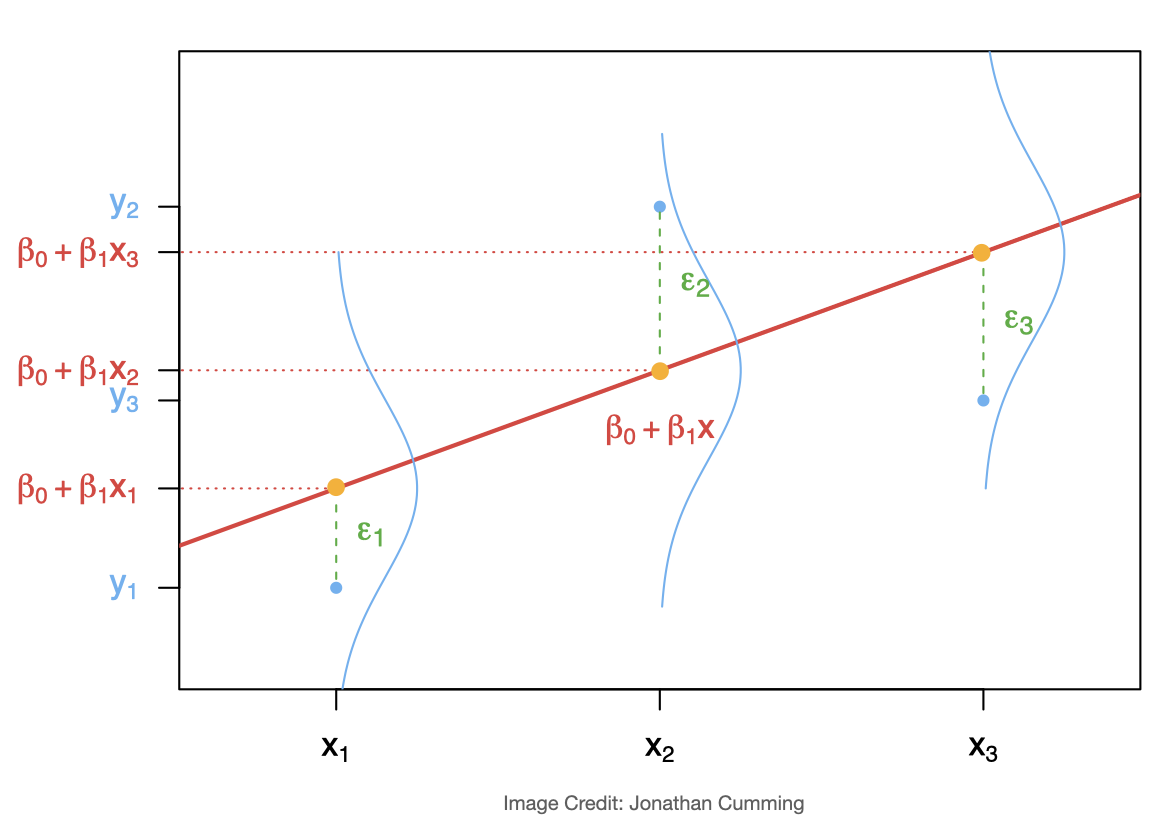
\includegraphics[width=0.6\linewidth,height=0.6\textheight]{figures/ass1} \end{center}

\hypertarget{example-used-cars-cont.-2}{%
\subsection{Example: used cars
(cont.)}\label{example-used-cars-cont.-2}}

\begin{center}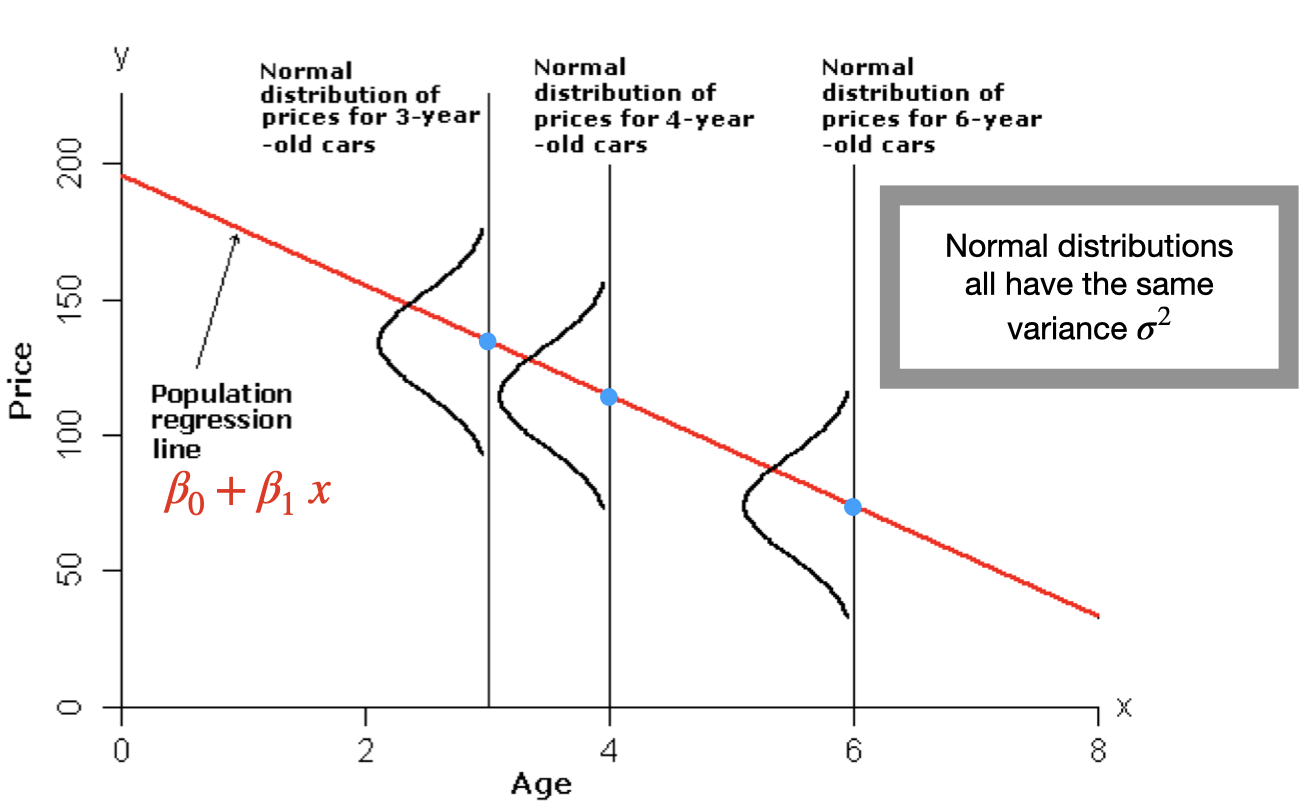
\includegraphics[width=0.6\linewidth,height=0.6\textheight]{figures/ass2} \end{center}

We can see that for each age, the mean price of all cars of that age
lies on the regression line \(E(Y|x)=\beta_0+\beta_1x\). And, the prices
of all cars of that age are assumed to be normally distributed with mean
equal to \(\beta_0+\beta_1 x\) and variance \(\sigma^2\). For example,
the prices of all 4-year-old cars must be normally distributed with mean
\(\beta_0+\beta_1 (4)\) and variance \(\sigma^2\).

We used the least square method to find the best fit for this data set,
and residuals can be obtained as
\(e_i=y_i-\hat{y_i}= y_i-(195.47 -20.26x_i)\).

\begin{center}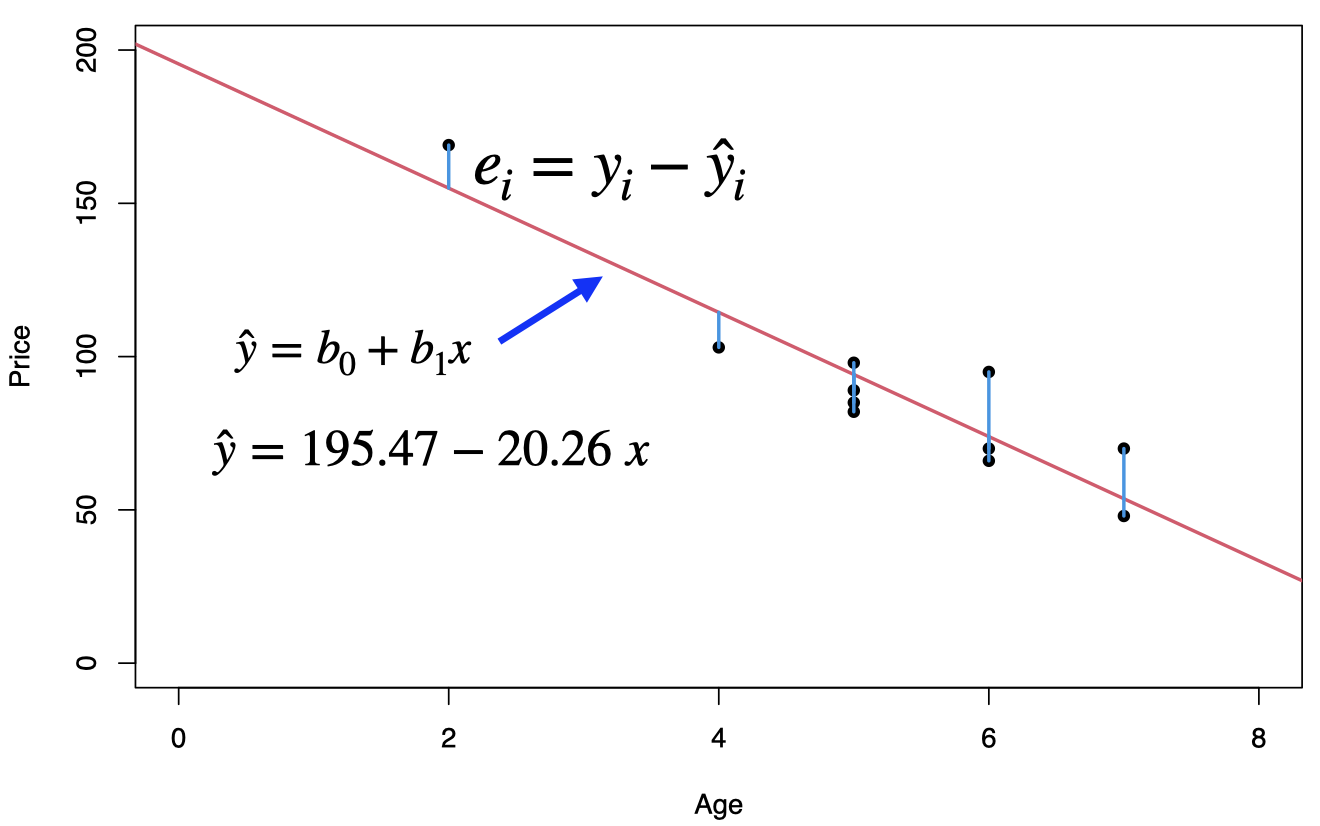
\includegraphics[width=0.6\linewidth,height=0.6\textheight]{figures/ass3} \end{center}

\hypertarget{residual-analysis}{%
\subsection{Residual Analysis}\label{residual-analysis}}

The easiest way to check the simple linear regression assumptions is by
constructing a scatterplot of the residuals (\(e_i=y_i-\hat{y_i}\))
against the fitted values (\(\hat{y_i}\)) or against \(x\). If the model
is a good fit, then the \textbf{residual plot} should show an even and
random scatter of the residuals.

\begin{center}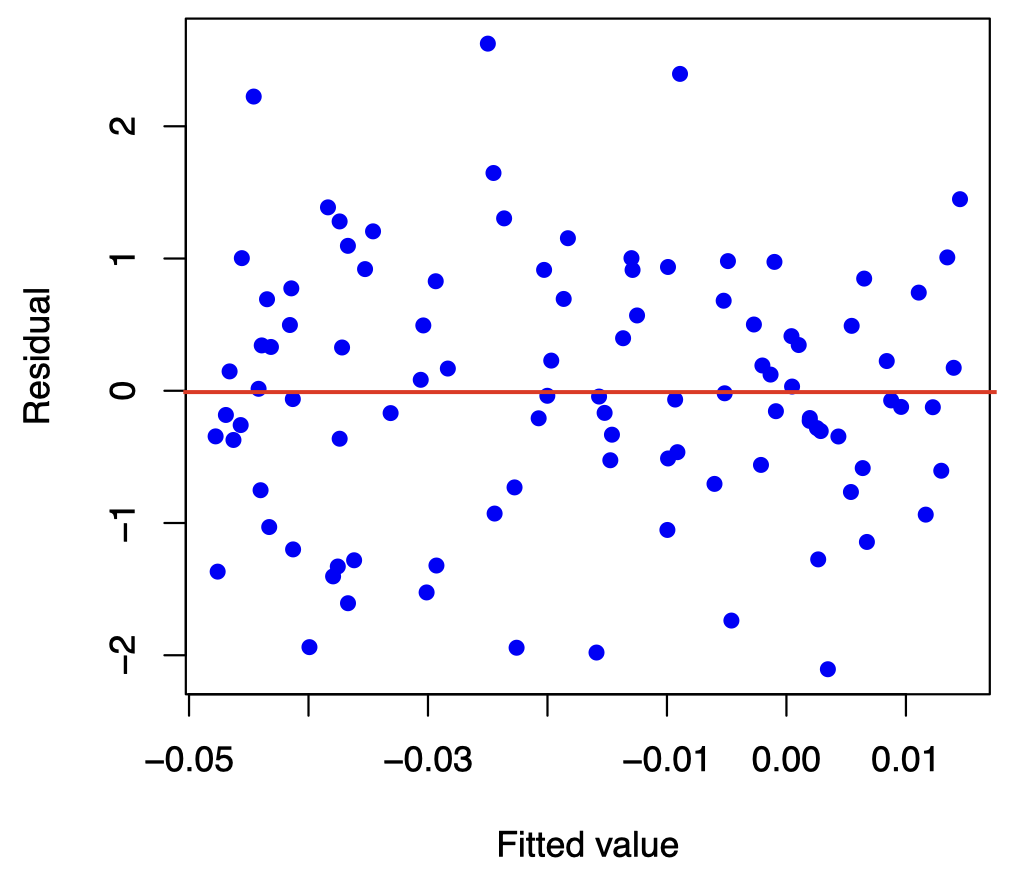
\includegraphics[width=0.4\linewidth,height=0.4\textheight]{figures/ass4} \end{center}

\hypertarget{linearity}{%
\subsubsection{Linearity}\label{linearity}}

The regression needs to be linear in the parameters.

\[Y=\beta_0+\beta_1\;x+\epsilon\]
\[E(Y_i|X_i)=\beta_0+\beta_1\;x_i  \equiv E(\epsilon_i|X_i)=E(\epsilon_i)=0\]

\begin{center}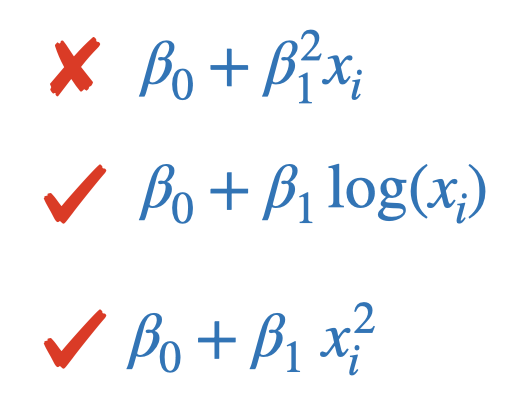
\includegraphics[width=0.15\linewidth,height=0.15\textheight]{figures/ass5} \end{center}

The residual plot below shows that a linear regression model is not
appropriate for this data.

\begin{center}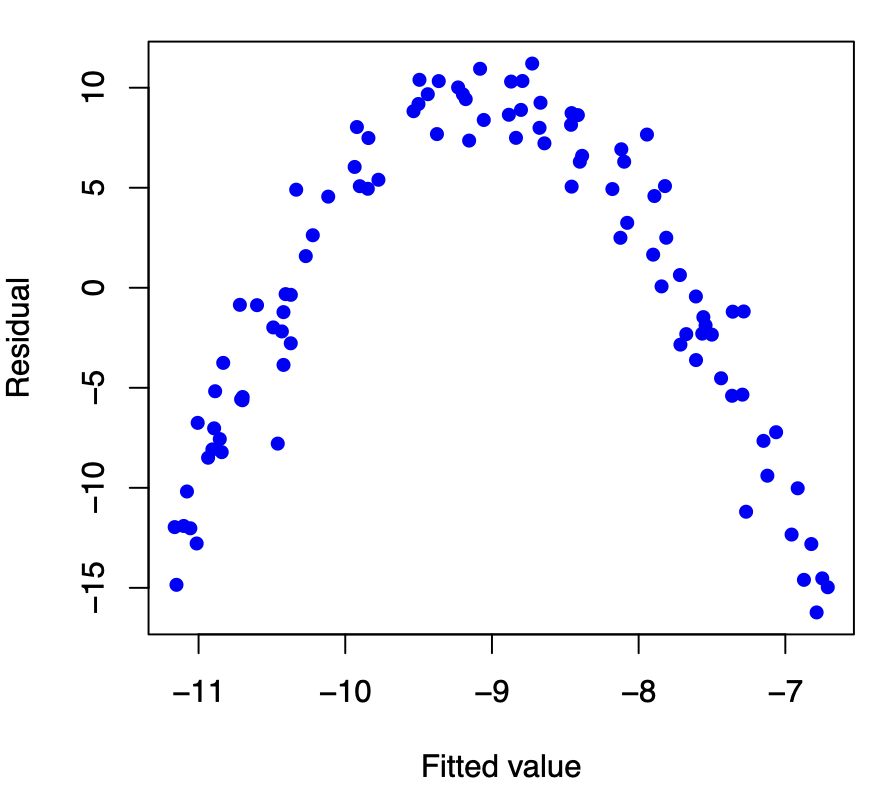
\includegraphics[width=0.4\linewidth,height=0.4\textheight]{figures/ass6} \end{center}

\hypertarget{constant-error-variance-homoscedasticity}{%
\subsubsection{Constant error variance
(homoscedasticity)}\label{constant-error-variance-homoscedasticity}}

The plot shows the spread of the residuals is increasing as the fitted
values (or \(x\)) increases, which indicates that we have
Heteroskedasticity (non-constant variance). The standard errors are
biased when heteroskedasticity is present, but the regression
coefficients will still be unbiased.

\begin{center}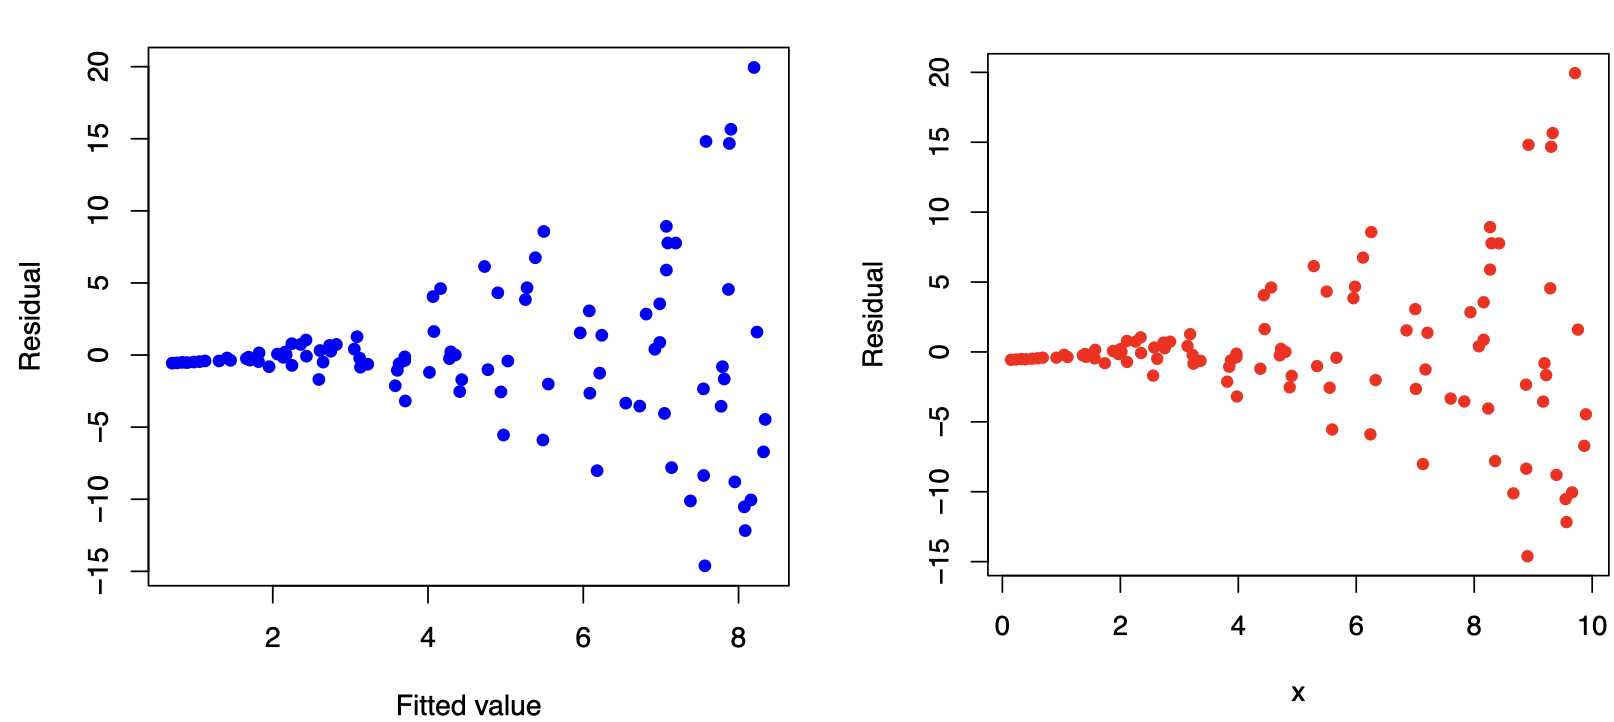
\includegraphics[width=0.7\linewidth,height=0.7\textheight]{figures/ass7} \end{center}

\textbf{How to detect?}

\begin{itemize}
\item
  Residuals plot (fitted vs residuals)
\item
  Goldfeld--Quandt test
\item
  Breusch-Pagan test
\end{itemize}

\textbf{How to fix?}

\begin{itemize}
\item
  White's standard errors
\item
  Weighted least squares model
\item
  Taking the log
\end{itemize}

\hypertarget{independent-errors-terms-no-autocorrelation}{%
\subsubsection{Independent errors terms (no
autocorrelation)}\label{independent-errors-terms-no-autocorrelation}}

The problem of autocorrelation is most likely to occur in time series
data, however, it can also occur in cross-sectional data, e.g.~if the
model is incorrectly specified. When autocorrelation is present, the
regression coefficients will still be unbiased, however, the standard
errors and test statitics are no longer valid.

\textbf{An example of no autocorrelation}

\begin{center}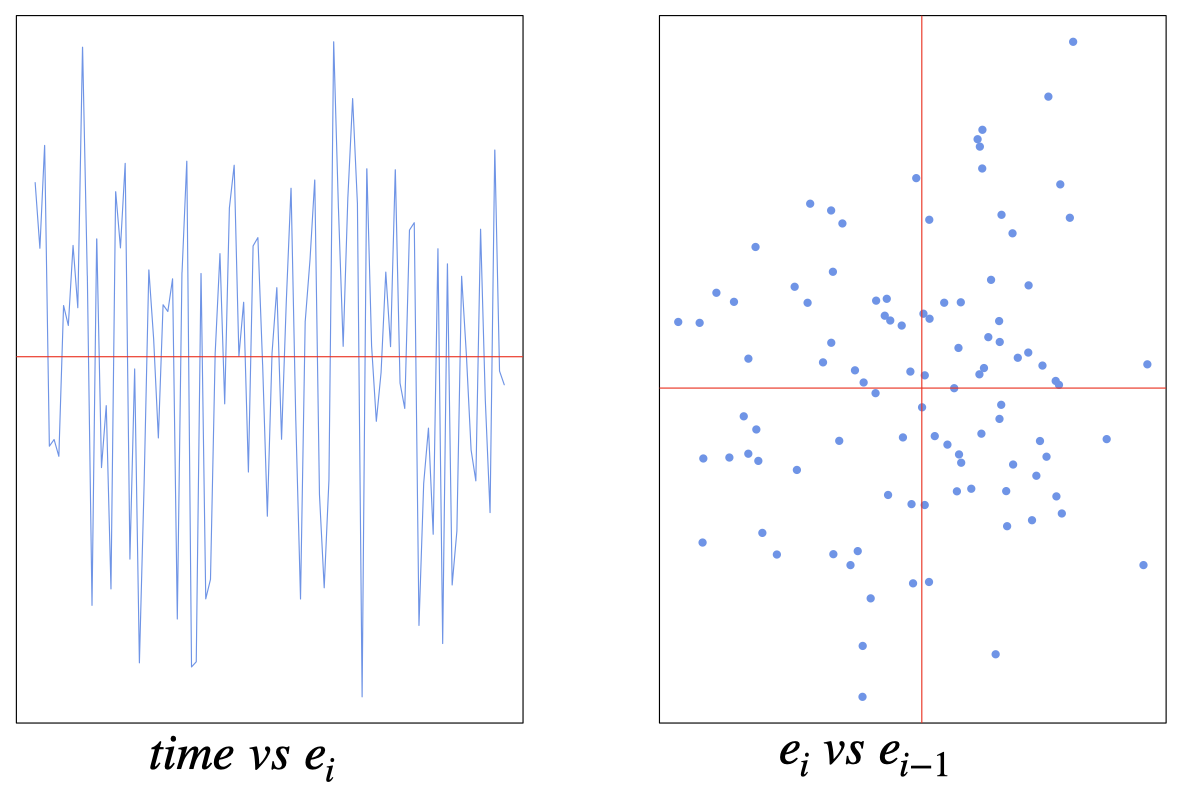
\includegraphics[width=0.6\linewidth,height=0.6\textheight]{figures/ass10} \end{center}

\textbf{An example of positive autocorrelation}

\begin{center}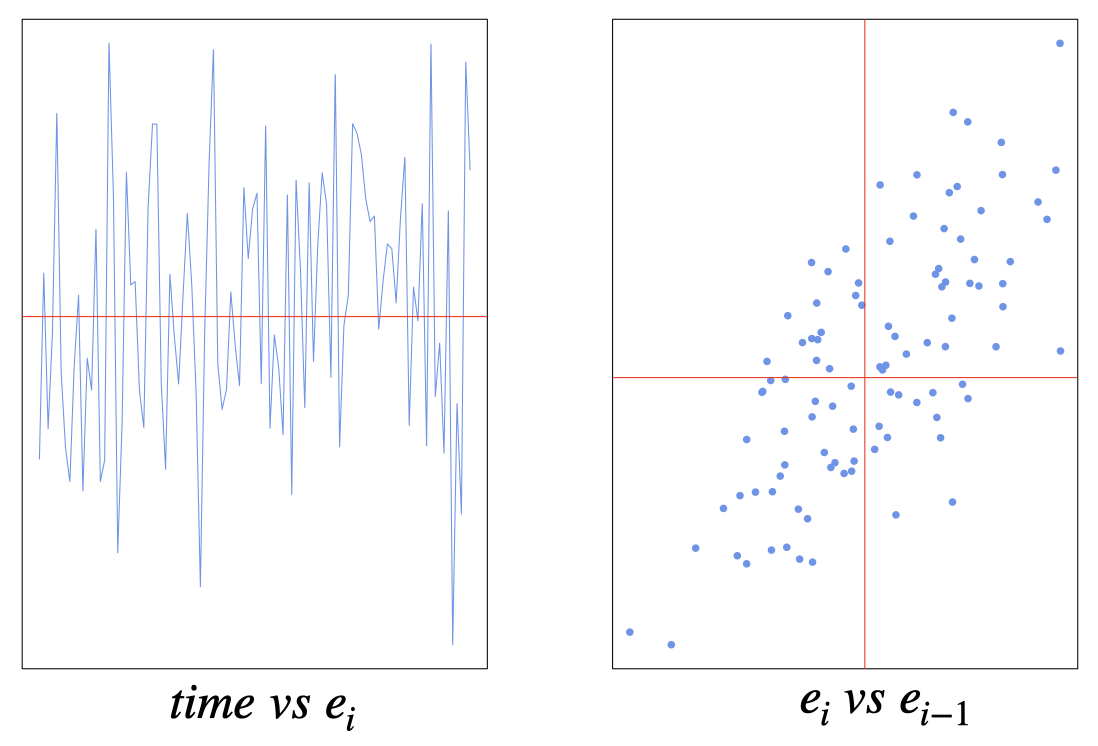
\includegraphics[width=0.6\linewidth,height=0.6\textheight]{figures/ass8} \end{center}

\textbf{An example of negative autocorrelation}

\begin{center}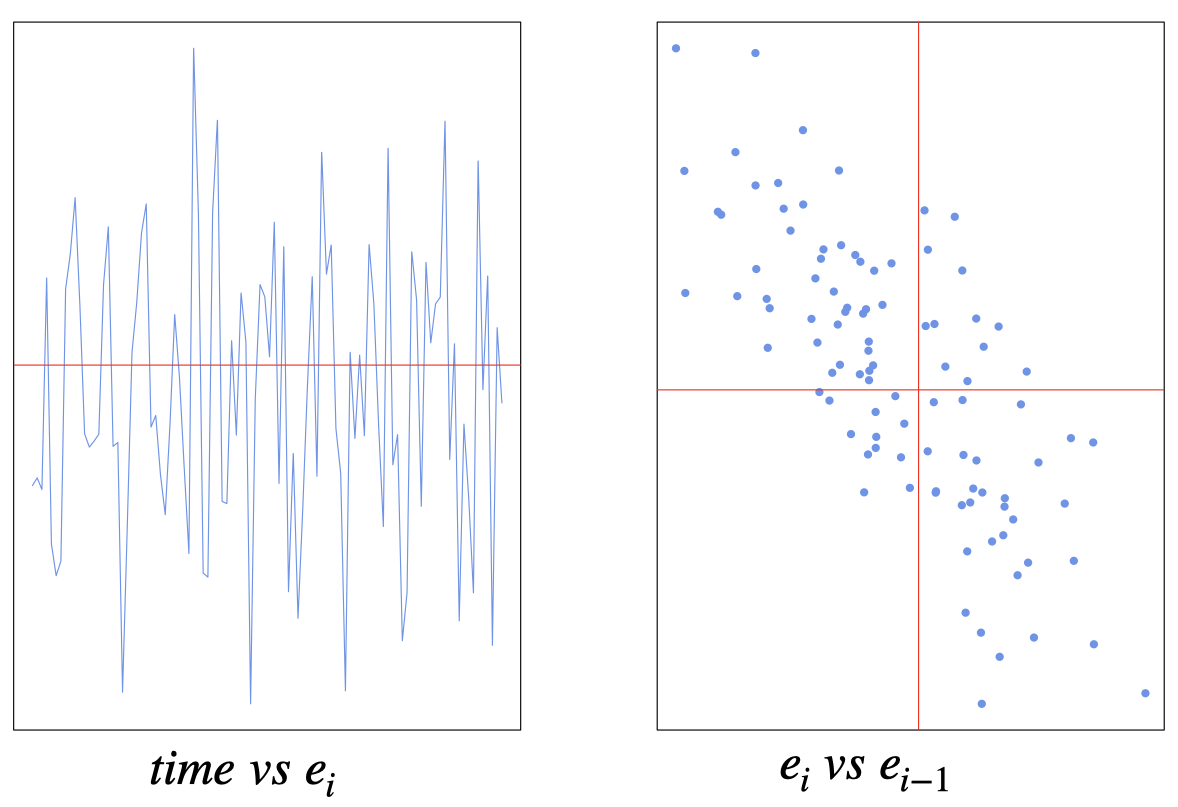
\includegraphics[width=0.6\linewidth,height=0.6\textheight]{figures/ass9} \end{center}

\textbf{How to detect?}

\begin{itemize}
\item
  Residuals plot
\item
  Durbin-Watson test
\item
  Breusch-Godfrey test
\end{itemize}

\textbf{How to fix?}

\begin{itemize}
\item
  Investigate omitted variables (e.g.~trend, business cycle)
\item
  Use advanced models (e.g.~AR model)
\end{itemize}

\hypertarget{normality-of-the-errors}{%
\subsubsection{Normality of the errors}\label{normality-of-the-errors}}

We need the errors to be normally distributed. Normality is only
required for the sampling distributions, hypothesis testing and
confidence intervals.

\textbf{How to detect?}

\begin{itemize}
\item
  Histogram of residuals
\item
  Q-Q plot of residuals
\item
  Kolmogorov--Smirnov test
\item
  Shapiro--Wilk test
\end{itemize}

\textbf{How to fix?}

\begin{itemize}
\item
  Change the functional form (e.g.~taking the log)
\item
  Larger sample if possible
\end{itemize}

\hypertarget{example-infant-mortality-and-gdp}{%
\subsection{Example: Infant mortality and
GDP}\label{example-infant-mortality-and-gdp}}

Let us investigate the relationship between infant mortality and the
wealth of a country. We will use data on 207 countries of the world
gathered by the UN in 1998 (the `UN' data set is available from the R
package `car'). The data set contains two variables: the infant
mortality rate in deaths per 1000 live births, and the GDP per capita in
US dollars. There are some missing data values for some countries, so we
will remove the missing data before we fit our model.

\begin{Shaded}
\begin{Highlighting}[]
\CommentTok{\# install.packages("carData")}
\FunctionTok{library}\NormalTok{(carData)}
\FunctionTok{data}\NormalTok{(UN)}
\FunctionTok{options}\NormalTok{(}\AttributeTok{scipen=}\DecValTok{999}\NormalTok{)}
\CommentTok{\# Remove missing data}
\NormalTok{newUN}\OtherTok{\textless{}{-}}\FunctionTok{na.omit}\NormalTok{(UN) }
\FunctionTok{str}\NormalTok{(newUN)}
\end{Highlighting}
\end{Shaded}

\begin{verbatim}
## 'data.frame':    193 obs. of  7 variables:
##  $ region         : Factor w/ 8 levels "Africa","Asia",..: 2 4 1 1 5 2 3 8 4 2 ...
##  $ group          : Factor w/ 3 levels "oecd","other",..: 2 2 3 3 2 2 2 1 1 2 ...
##  $ fertility      : num  5.97 1.52 2.14 5.13 2.17 ...
##  $ ppgdp          : num  499 3677 4473 4322 9162 ...
##  $ lifeExpF       : num  49.5 80.4 75 53.2 79.9 ...
##  $ pctUrban       : num  23 53 67 59 93 64 47 89 68 52 ...
##  $ infantMortality: num  124.5 16.6 21.5 96.2 12.3 ...
##  - attr(*, "na.action")= 'omit' Named int [1:20] 4 6 21 35 38 54 67 75 77 78 ...
##   ..- attr(*, "names")= chr [1:20] "American Samoa" "Anguilla" "Bermuda" "Cayman Islands" ...
\end{verbatim}

\begin{Shaded}
\begin{Highlighting}[]
\NormalTok{fit}\OtherTok{\textless{}{-}} \FunctionTok{lm}\NormalTok{(infantMortality }\SpecialCharTok{\textasciitilde{}}\NormalTok{ ppgdp, }\AttributeTok{data=}\NormalTok{newUN)}
\FunctionTok{summary}\NormalTok{(fit)}
\end{Highlighting}
\end{Shaded}

\begin{verbatim}
## 
## Call:
## lm(formula = infantMortality ~ ppgdp, data = newUN)
## 
## Residuals:
##    Min     1Q Median     3Q    Max 
## -31.48 -18.65  -8.59  10.86  83.59 
## 
## Coefficients:
##               Estimate Std. Error t value             Pr(>|t|)    
## (Intercept) 41.3780016  2.2157454  18.675 < 0.0000000000000002 ***
## ppgdp       -0.0008656  0.0001041  -8.312   0.0000000000000173 ***
## ---
## Signif. codes:  0 '***' 0.001 '**' 0.01 '*' 0.05 '.' 0.1 ' ' 1
## 
## Residual standard error: 25.13 on 191 degrees of freedom
## Multiple R-squared:  0.2656, Adjusted R-squared:  0.2618 
## F-statistic: 69.08 on 1 and 191 DF,  p-value: 0.0000000000000173
\end{verbatim}

\begin{Shaded}
\begin{Highlighting}[]
\FunctionTok{plot}\NormalTok{(newUN}\SpecialCharTok{$}\NormalTok{infantMortality }\SpecialCharTok{\textasciitilde{}}\NormalTok{ newUN}\SpecialCharTok{$}\NormalTok{ppgdp, }\AttributeTok{xlab=}\StringTok{"GDP per Capita"}\NormalTok{, }\AttributeTok{ylab=}\StringTok{"Infant mortality (per 1000 births)"}\NormalTok{, }\AttributeTok{pch=}\DecValTok{16}\NormalTok{, }\AttributeTok{col=}\StringTok{"cornflowerblue"}\NormalTok{)}
\FunctionTok{abline}\NormalTok{(fit,}\AttributeTok{col=}\StringTok{"red"}\NormalTok{)}
\end{Highlighting}
\end{Shaded}

\begin{center}\includegraphics[width=0.6\linewidth,height=0.6\textheight]{unnamed-chunk-59-1} \end{center}

We can see from the scatterplot that the relationship between the two
variables is not linear. There is a concentration of data points at
small values of GDP (many poor countries) and a concentration of data
points at small values of infant mortality (many countries with very low
mortality). This suggests a skewness to both variables which would not
conform to the normality assumption. Indeed, the regression line (the
red line) we construct is a poor fit and only has an \(R^2\) of 0.266.

From the residual plot below we can see a clear evidence of structure to
the residuals suggesting the linear relationship is a poor description
of the data, and substantial changes in spread suggesting the assumption
of homogeneous variance is not appropriate.

\begin{Shaded}
\begin{Highlighting}[]
\CommentTok{\# diagnostic plots }
\FunctionTok{plot}\NormalTok{(fit,}\AttributeTok{which=}\DecValTok{1}\NormalTok{,}\AttributeTok{pch=}\DecValTok{16}\NormalTok{,}\AttributeTok{col=}\StringTok{"cornflowerblue"}\NormalTok{)}
\end{Highlighting}
\end{Shaded}

\begin{center}\includegraphics[width=0.6\linewidth,height=0.6\textheight]{unnamed-chunk-60-1} \end{center}

So we can apply a transformation to one or both variables, e.g.~taking
the log or adding a quadratic form. Notice that this will not affect
(violet) the linearity assumption as the regression will still be linear
in the parameters. So if we take the logs of both variables gives us the
scatterplot of the transformed data set, below, which appears to show a
more promising linear structure. The quality of the regression is now
improved, with an \(R^2\) value of 0.766, which is still a little weak
due to the rather large spread in the data.

\begin{Shaded}
\begin{Highlighting}[]
\NormalTok{fit1}\OtherTok{\textless{}{-}} \FunctionTok{lm}\NormalTok{(}\FunctionTok{log}\NormalTok{(infantMortality) }\SpecialCharTok{\textasciitilde{}} \FunctionTok{log}\NormalTok{(ppgdp), }\AttributeTok{data=}\NormalTok{newUN)}
\FunctionTok{summary}\NormalTok{(fit1)}
\end{Highlighting}
\end{Shaded}

\begin{verbatim}
## 
## Call:
## lm(formula = log(infantMortality) ~ log(ppgdp), data = newUN)
## 
## Residuals:
##      Min       1Q   Median       3Q      Max 
## -1.16789 -0.36738 -0.02351  0.24544  2.43503 
## 
## Coefficients:
##             Estimate Std. Error t value            Pr(>|t|)    
## (Intercept)  8.10377    0.21087   38.43 <0.0000000000000002 ***
## log(ppgdp)  -0.61680    0.02465  -25.02 <0.0000000000000002 ***
## ---
## Signif. codes:  0 '***' 0.001 '**' 0.01 '*' 0.05 '.' 0.1 ' ' 1
## 
## Residual standard error: 0.5281 on 191 degrees of freedom
## Multiple R-squared:  0.7662, Adjusted R-squared:  0.765 
## F-statistic: 625.9 on 1 and 191 DF,  p-value: < 0.00000000000000022
\end{verbatim}

\begin{Shaded}
\begin{Highlighting}[]
\FunctionTok{plot}\NormalTok{(}\FunctionTok{log}\NormalTok{(newUN}\SpecialCharTok{$}\NormalTok{infantMortality) }\SpecialCharTok{\textasciitilde{}} \FunctionTok{log}\NormalTok{(newUN}\SpecialCharTok{$}\NormalTok{ppgdp), }\AttributeTok{xlab=}\StringTok{"GDP per Capita"}\NormalTok{, }\AttributeTok{ylab=}\StringTok{"Infant mortality (per 1000 births)"}\NormalTok{, }\AttributeTok{pch=}\DecValTok{16}\NormalTok{, }\AttributeTok{col=}\StringTok{"cornflowerblue"}\NormalTok{)}
\FunctionTok{abline}\NormalTok{(fit1,}\AttributeTok{col=}\StringTok{"red"}\NormalTok{)}
\end{Highlighting}
\end{Shaded}

%\begin{center}\includegraphics[width=0.6\linewidth,height=0.6\textheight]{unnamed-chunk-61-1} \end{center}

So we check the residuals again, as we can see from the residuals plot
below that the log transformation has corrected many of the problems
with with residual plot and the residuals now much closer to the
expected random scatter.

\begin{Shaded}
\begin{Highlighting}[]
\CommentTok{\# diagnostic plots }
\FunctionTok{plot}\NormalTok{(fit1,}\AttributeTok{which=}\DecValTok{1}\NormalTok{,}\AttributeTok{pch=}\DecValTok{16}\NormalTok{,}\AttributeTok{col=}\StringTok{"cornflowerblue"}\NormalTok{)}
\end{Highlighting}
\end{Shaded}

\begin{center}\includegraphics[width=0.6\linewidth,height=0.6\textheight]{unnamed-chunk-62-1} \end{center}

Now let us check the Normality of the errors by creating a histogram and
normal QQ plot for the residuals, before and after the log
transformation. The normal quantile (QQ) plot shows the sample quantiles
of the residuals against the theoretical quantiles that we would expect
if these values were drawn from a Normal distribution. If the Normal
assumption holds, then we would see an approximate straight-line
relationship on the Normal quantile plot.

\begin{Shaded}
\begin{Highlighting}[]
\FunctionTok{par}\NormalTok{(}\AttributeTok{mfrow=}\FunctionTok{c}\NormalTok{(}\DecValTok{2}\NormalTok{,}\DecValTok{2}\NormalTok{))}
\CommentTok{\# before the log  transformation.}
\FunctionTok{plot}\NormalTok{(fit, }\AttributeTok{which =} \DecValTok{2}\NormalTok{,}\AttributeTok{pch=}\DecValTok{16}\NormalTok{, }\AttributeTok{col=}\StringTok{"cornflowerblue"}\NormalTok{)}
\FunctionTok{hist}\NormalTok{(}\FunctionTok{resid}\NormalTok{(fit),}\AttributeTok{col=}\StringTok{"cornflowerblue"}\NormalTok{,}\AttributeTok{main=}\StringTok{""}\NormalTok{)}
\CommentTok{\# after the log  transformation.}
\FunctionTok{plot}\NormalTok{(fit1, }\AttributeTok{which =} \DecValTok{2}\NormalTok{, }\AttributeTok{pch=}\DecValTok{16}\NormalTok{, }\AttributeTok{col=}\StringTok{"hotpink3"}\NormalTok{)  }
\FunctionTok{hist}\NormalTok{(}\FunctionTok{resid}\NormalTok{(fit1),}\AttributeTok{col=}\StringTok{"hotpink3"}\NormalTok{,}\AttributeTok{main=}\StringTok{""}\NormalTok{)}
\end{Highlighting}
\end{Shaded}

%\begin{center}\includegraphics[width=0.9\linewidth,height=0.9\textheight]{unnamed-chunk-63-1} \end{center}

The normal quantile plot and the histogram of residuals (before the log
transformation) shows strong departure from the expectation of an
approximate straight line, with curvature in the tails which reflects
the skewness of the data. Finally, the normal quantile plot and the
histogram of residuals suggest that residuals are much closer to
Normality after the transformation, with some minor deviations in the
tails.

\hypertarget{simple-linear-regression-inference}{%
\section{Simple Linear Regression:
Inference}\label{simple-linear-regression-inference}}

\hypertarget{simple-linear-regression-assumptions-1}{%
\subsection{Simple Linear Regression
Assumptions}\label{simple-linear-regression-assumptions-1}}

\begin{itemize}
\item
  Linearity of the relationship between the dependent and independent
  variables
\item
  Independence of the errors (no autocorrelation)
\item
  Constant variance of the errors (homoscedasticity)
\item
  Normality of the error distribution.
\end{itemize}

\hypertarget{simple-linear-regression-2}{%
\subsection{Simple Linear Regression}\label{simple-linear-regression-2}}

The simple linear regression model for \(Y\) on \(x\) is
\[Y=\beta_0+\beta_1 x+\epsilon\] where

\(Y\) : the dependent or response variable

\(x\) : the independent or predictor variable, assumed known

\(\beta_0,\beta_1\) : the regression parameters, the intercept and slope
of the regression line

\(\epsilon\) : the random regression error around the line.

\hypertarget{the-simple-linear-regression-equation}{%
\subsection{The simple linear regression
equation}\label{the-simple-linear-regression-equation}}

\begin{itemize}
\tightlist
\item
  The regression equation for a set of \(n\) data points is
  \(\hat{y}=b_0+b_1\;x\), where
  \[b_1=\frac{S_{xy}}{S_{xx}}=\frac{\sum (x_i-\bar{x})(y_i-\bar{y})}{\sum (x_i-\bar{x})^2}\]
  and \[b_0=\bar{y}-b_1\; \bar{x}\]
\item
  \(y\) is the dependent variable (or response variable) and \(x\) is
  the independent variable (predictor variable or explanatory variable).
\item
  \(b_0\) is called the \textbf{y-intercept} and \(b_1\) is called the
  \textbf{slope}.
\end{itemize}

\hypertarget{residual-standard-error-s_e}{%
\subsection{\texorpdfstring{Residual standard error,
\(s_e\)}{Residual standard error, s\_e}}\label{residual-standard-error-s_e}}

The residual standard error, \(s_e\), is defined by
\[s_e=\sqrt{\frac{SSE}{n-2}}\] where \(SSE\) is the error sum of squares
(also known as the residual sum of squares, RSS) which can be defined as
\[SSE=\sum e^2_i=\sum(y_i-\hat{y}_i)^2=S_{yy}-\frac{S^2_{xy}}{S_{xx}}\]
\(s_e\) indicates how much, on average, the observed values of the
response variable differ from the predicated values of the response
variable. Under the simple linear regression assumptions, \(s_e\) is an
unbiased estimate for the error standard deviation \(\sigma\).

\hypertarget{properties-of-regression-coefficients}{%
\subsection{Properties of Regression
Coefficients}\label{properties-of-regression-coefficients}}

Under the simple linear regression assumptions, the least square
estimates \(b_0\) and \(b_1\) are unbiased for the \(\beta_0\) and
\(\beta_1\), respectively, i.e.

\(E[b_0]=\beta_0\) and \(E[b_1]=\beta_1\).

The variances of the least squares estimators in simple linear
regression are:

\[Var[b_0]=\sigma^2_{b_0}=\sigma^2\left(\frac{1}{n}+\frac{\bar{x}^2}{S_{xx}}\right)\]

\[Var[b_1]=\sigma^2_{b_1}=\frac{\sigma^2}{S_{xx}}\]
\[Cov[b_0,b_1]=\sigma_{b_0,b_1}=-\sigma^2\frac{\bar{x}}{S_{xx}}\]

We use \(s_e\) to estimate the error standard deviation \(\sigma\):

\[s^2_{b_0}=s_e^2\left(\frac{1}{n}+\frac{\bar{x}^2}{S_{xx}}\right)\]

\[s^2_{b_1}=\frac{s_e^2}{S_{xx}}\]

\[s_{b_0,b_1}=-s_e^2\frac{\bar{x}}{S_{xx}}\]

\hypertarget{sampling-distribution-of-the-least-square-estimators}{%
\subsection{Sampling distribution of the least square
estimators}\label{sampling-distribution-of-the-least-square-estimators}}

For the Normal error simple linear regression model:
\[b_0\sim N(\beta_0,\sigma^2_{b_0}) \rightarrow 
\frac{b_0-\beta_0}{\sigma_{b_0}}\sim N(0,1)\] and
\[b_1\sim N(\beta_1,\sigma^2_{b_1}) \rightarrow
\frac{b_1-\beta_1}{\sigma_{b_1}}\sim N(0,1)\]

We use \(s_e\) to estimate the error standard deviation \(\sigma\):
\[\frac{b_0-\beta_0}{s_{b_0}}\sim t_{n-2}\] and
\[\frac{b_1-\beta_1}{s_{b_1}}\sim t_{n-2}\]

\hypertarget{degrees-of-freedom}{%
\subsection{Degrees of Freedom}\label{degrees-of-freedom}}

\begin{itemize}
\item
  In statistics, degrees of freedom are the number of independent pieces
  of information that go into the estimate of a particular parameter.
\item
  Typically, the degrees of freedom of an estimate of a parameter are
  equal to the number of independent observations that go into the
  estimate, minus the number of parameters that are estimated as
  intermediate steps in the estimation of the parameter itself.
\item
  The sample variance has \(n - 1\) degrees of freedom, since it is
  computed from n pieces of data, minus the 1 parameter estimated as
  intermediate step, the sample mean. Similarly, having estimated the
  sample mean we only have \(n - 1\) independent pieces of data left, as
  if we are given the sample mean and any \(n - 1\) of the observations
  then we can determine the value of remaining observation exactly.
\end{itemize}

\[s^2=\frac{\sum(x_i-\bar{x})^2}{n-1}\]

\begin{itemize}
\tightlist
\item
  In linear regression, the degrees of freedom of the residuals is
  \(df=n-k^*\), where \(k^*\) is the numbers of estimated parameters
  (including the intercept). So for the simple linear regression, we are
  estimating \(\beta_0\) and \(\beta_1\), thus \(df=n-2\).
\end{itemize}

\hypertarget{inference-for-the-intercept-beta_0}{%
\subsection{\texorpdfstring{Inference for the intercept
\(\beta_0\)}{Inference for the intercept \textbackslash beta\_0}}\label{inference-for-the-intercept-beta_0}}

\begin{itemize}
\item
  Hypotheses:\[H_0:\beta_0=0\;\; \text{against}\;\; H_1:\beta_0\neq 0\]
\item
  Test statistic: \[t=\frac{b_0}{s_{b_0}}\] has a t-distribution with
  \(df=n-2\), where \(s_{b_0}\) is the standard error of \(b_0\), and
  given by \[s_{b_0}=s_e\sqrt{\frac{1}{n}+\frac{\bar{x}^2}{S_{xx}}}\]
  and
\end{itemize}

\[s_e=\sqrt{\frac{SSE}{n-2}}=\sqrt{\frac{\sum(y_i-\hat{y}_i)^2}{n-2}}\]
We reject \(H_0\) at level \(\alpha\) if \(|t|>t_{\alpha/2}\) with
\(df=n-2\).

\begin{itemize}
\tightlist
\item
  100(1-\(\alpha\))\% confidence interval for \(\beta_0\),
\end{itemize}

\[b_0 \pm t_{\alpha/2} .\;s_{b_0}\] where \(t_{\alpha/2}\) is critical
value obtained from the t‐distribution table with \(df=n-2\).

\hypertarget{inference-for-the-slope-beta_1}{%
\subsection{\texorpdfstring{Inference for the slope
\(\beta_1\)}{Inference for the slope \textbackslash beta\_1}}\label{inference-for-the-slope-beta_1}}

\begin{itemize}
\item
  Hypotheses: \[H_0:\beta_1=0\;\; \text{against}\;\; H_1:\beta_1\neq 0\]
\item
  Test statistic: \[t=\frac{b_1}{s_{b_1}}\] has a t-distribution with
  \(df=n-2\), where \(s_{b_1}\) is the standard error of \(b_1\),and
  given by
\end{itemize}

\[s_{b_1}=\frac{s_e}{\sqrt{S_{xx}}}\]

and

\[s_e=\sqrt{\frac{SSE}{n-2}}=\sqrt{\frac{\sum(y_i-\hat{y}_i)^2}{n-2}}\]
We reject \(H_0\) at level \(\alpha\) if \(|t|>t_{\alpha/2}\) with
\(df=n-2\).

\begin{itemize}
\tightlist
\item
  100(1-\(\alpha\))\% confidence interval for \(\beta_1\),
\end{itemize}

\[b_1 \pm t_{\alpha/2} \;s_{b_1}\] where \(t_{\alpha/2}\) is critical
value obtained from the t‐distribution table with \(df=n-2\).

\begin{center}\includegraphics[width=0.3\linewidth,height=0.3\textheight]{figures/Ttest2} \end{center}

\hypertarget{how-useful-is-the-regression-model}{%
\subsection{How useful is the regression
model?}\label{how-useful-is-the-regression-model}}

\textbf{Goodness of fit test}

\begin{itemize}
\item
  We test the null hypothesis \(H_0:\beta_1=0\) against
  \(H_1:\beta_1\neq 0\), the F-statistic
  \[F=\frac{MSR}{MSE}=\frac{SSR}{SSE/(n-2)}\] has F-distribution with
  degrees of freedom \(df_1=1\) and \(df_2=n-2\).
\item
  We reject \(H_0\), at level \(\alpha\), if
  \(F>F_{\alpha}(df_1,df_2)\).
\item
  For a simple linear regression ONLY, F-test is equivalent to t-test
  for \(\beta_1\).
\end{itemize}

\begin{center}\includegraphics[width=0.4\linewidth,height=0.4\textheight]{figures/Ftest} \end{center}

\hypertarget{example-used-cars-cont.-3}{%
\subsection{Example: used cars
(cont.)}\label{example-used-cars-cont.-3}}

\begin{Shaded}
\begin{Highlighting}[]
\NormalTok{Price}\OtherTok{\textless{}{-}}\FunctionTok{c}\NormalTok{(}\DecValTok{85}\NormalTok{, }\DecValTok{103}\NormalTok{,  }\DecValTok{70}\NormalTok{,  }\DecValTok{82}\NormalTok{,  }\DecValTok{89}\NormalTok{,  }\DecValTok{98}\NormalTok{,  }\DecValTok{66}\NormalTok{,  }\DecValTok{95}\NormalTok{, }\DecValTok{169}\NormalTok{,  }\DecValTok{70}\NormalTok{,  }\DecValTok{48}\NormalTok{)}
\NormalTok{Age}\OtherTok{\textless{}{-}} \FunctionTok{c}\NormalTok{(}\DecValTok{5}\NormalTok{, }\DecValTok{4}\NormalTok{, }\DecValTok{6}\NormalTok{, }\DecValTok{5}\NormalTok{, }\DecValTok{5}\NormalTok{, }\DecValTok{5}\NormalTok{, }\DecValTok{6}\NormalTok{, }\DecValTok{6}\NormalTok{, }\DecValTok{2}\NormalTok{, }\DecValTok{7}\NormalTok{, }\DecValTok{7}\NormalTok{)}
\NormalTok{carSales}\OtherTok{\textless{}{-}}\FunctionTok{data.frame}\NormalTok{(Price,Age)}
\FunctionTok{str}\NormalTok{(carSales)}
\end{Highlighting}
\end{Shaded}

\begin{verbatim}
## 'data.frame':    11 obs. of  2 variables:
##  $ Price: num  85 103 70 82 89 98 66 95 169 70 ...
##  $ Age  : num  5 4 6 5 5 5 6 6 2 7 ...
\end{verbatim}

\begin{Shaded}
\begin{Highlighting}[]
\CommentTok{\# simple linear regression}
\NormalTok{reg}\OtherTok{\textless{}{-}}\FunctionTok{lm}\NormalTok{(Price}\SpecialCharTok{\textasciitilde{}}\NormalTok{Age)}
\FunctionTok{summary}\NormalTok{(reg)}
\end{Highlighting}
\end{Shaded}

\begin{verbatim}
## 
## Call:
## lm(formula = Price ~ Age)
## 
## Residuals:
##     Min      1Q  Median      3Q     Max 
## -12.162  -8.531  -5.162   8.946  21.099 
## 
## Coefficients:
##             Estimate Std. Error t value    Pr(>|t|)    
## (Intercept)   195.47      15.24  12.826 0.000000436 ***
## Age           -20.26       2.80  -7.237 0.000048819 ***
## ---
## Signif. codes:  0 '***' 0.001 '**' 0.01 '*' 0.05 '.' 0.1 ' ' 1
## 
## Residual standard error: 12.58 on 9 degrees of freedom
## Multiple R-squared:  0.8534, Adjusted R-squared:  0.8371 
## F-statistic: 52.38 on 1 and 9 DF,  p-value: 0.00004882
\end{verbatim}

\(~\)

\begin{Shaded}
\begin{Highlighting}[]
\CommentTok{\# To obtain the confidence intervals }
\FunctionTok{confint}\NormalTok{(reg, }\AttributeTok{level=}\FloatTok{0.95}\NormalTok{)}
\end{Highlighting}
\end{Shaded}

\begin{verbatim}
##                 2.5 %    97.5 %
## (Intercept) 160.99243 229.94451
## Age         -26.59419 -13.92833
\end{verbatim}

\hypertarget{r-output}{%
\subsection{R output}\label{r-output}}

\begin{center}\includegraphics[width=0.8\linewidth,height=0.8\textheight]{figures/regRoutput} \end{center}

\hypertarget{simple-linear-regression-confidence-and-prediction-intervals}{%
\section{Simple Linear Regression: Confidence and Prediction
intervals}\label{simple-linear-regression-confidence-and-prediction-intervals}}

Earlier we have introduced the simple linear regression as a basic
statistical model for the relationship between two random variables. We
used the least square method for estimating the regression parameters.

Recall that the simple linear regression model for \(Y\) on \(x\) is
\[Y=\beta_0+\beta_1 x+\epsilon\] where

\(Y\) : the dependent or response variable

\(x\) : the independent or predictor variable, assumed known

\(\beta_0,\beta_1\) : the regression parameters, the intercept and slope
of the regression line

\(\epsilon\) : the random regression error around the line.

and the regression equation for a set of \(n\) data points is
\(\hat{y}=b_0+b_1\;x\), where
\[b_1=\frac{S_{xy}}{S_{xx}}=\frac{\sum (x_i-\bar{x})(y_i-\bar{y})}{\sum (x_i-\bar{x})^2}\]
and \[b_0=\bar{y}-b_1\; \bar{x}\] where \(b_0\) is called the
\textbf{y-intercept} and \(b_1\) is called the \textbf{slope}.

\(~\)

\textbf{Under the simple linear regression assumptions}, the residual
standard error \(s_e\) is an unbiased estimate for the error standard
deviation \(\sigma\), where

\[s_e=\sqrt{\frac{SSE}{n-2}}=\sqrt{\frac{\sum(y_i-\hat{y}_i)^2}{n-2}} \]
\(s_e\) indicates how much, on average, the observed values of the
response variable differ from the predicated values of the response
variable.

\(~\)

Below we will see how we can use these least square estimates for
prediction. First, we will consider the inference for the conditional
mean of the response variable \(y\) given a particular value of the
independent variable \(x\), let us call this particular value \(x^*\).
Next we will see how to predicting the value of the response variable
\(Y\) for a given value of the independent variable \(x^*\). These
confidence and predictive intervals, to be valid, the usual four simple
regression assumptions must hold.

\hypertarget{inference-for-the-regression-line-eleftyxright}{%
\subsection{\texorpdfstring{Inference for the regression line
\(E\left[Y|x^*\right]\)}{Inference for the regression line E\textbackslash left{[}Y\textbar x\^{}*\textbackslash right{]}}}\label{inference-for-the-regression-line-eleftyxright}}

Suppose we are interested in the value of the regression line at a new
point \(x^*\). Let's denote the unknown true value of the regression
line at \(x=x^*\) as \(\mu^*\). From the form of the regression line
equation we have

\[\mu^*=\mu_{Y|x^*}=E\left[Y|x^*\right]=\beta_0+\beta_1 x^*\]

but \(\beta_0\) and \(\beta_1\) are unknown. We can use the least square
regression equation to estimate the unknown true value of the regression
line, so we have

\[\hat{\mu}^*=b_0+b_1 x^*=\hat{y}^*\]

This is simply a point estimate for the regression line. However, in
statistics, point estimate is often not enough, and we need to express
our uncertainty about this point estimate, and one way to do so is via
confidence interval.

A \(100(1-\alpha)\%\) confidence interval for the conditional mean
\(\mu^*\) is
\[\hat{y}^*\pm t_{\alpha/2}\;\cdot s_e\;\sqrt{\frac{1}{n}+\frac{(x^*-\bar{x})^2}{S_{xx}}}\]
where \(S_{xx}=\sum_{i=1}^{n} (x_i-\bar{x})^2\), and \(t_{\alpha/2}\) is
the \(\alpha/2\) critical value from the t-distribution with \(df=n-2\).

\begin{center}\includegraphics[width=0.35\linewidth,height=0.35\textheight]{figures/Ttest2} \end{center}

\hypertarget{inference-for-the-response-variable-y-for-a-given-xx}{%
\subsection{\texorpdfstring{Inference for the response variable \(Y\)
for a given
\(x=x^*\)}{Inference for the response variable Y for a given x=x\^{}*}}\label{inference-for-the-response-variable-y-for-a-given-xx}}

Suppose now we are interested in predicting the value of \(Y^*\) if we
have a new observation at \(x^*\).

At \(x=x^*\), the value of \(Y^*\) is unknown and given by
\[Y^*=\beta_0+\beta_1 x^*+\epsilon\] where but \(\beta_0\), \(\beta_1\)
and \(\epsilon\) are unknown. We will use \(\hat{y}^*=b_0+b_1\;x^*\) as
a basis for our prediction.

\(~\)

A \(100(1-\alpha)\%\) prediction interval for \(Y^*\) at \(x=x^*\) is

\[\hat{y}^* \pm t_{\alpha/2}\;\cdot s_e\;\sqrt{1+\frac{1}{n}+\frac{(x^*-\bar{x})^2}{S_{xx}}}\]
The extra '1' under the square root sign, we have here to account for
the extra variability of a single observation about the mean.

Note: we construct a confidence interval for a parameter of the
population, which is the conditional mean in this case, while we
construct a prediction interval for a single value.

\hypertarget{example-used-cars-cont.-4}{%
\subsection{Example: used cars
(cont.)}\label{example-used-cars-cont.-4}}

\textbf{Estimate the mean price of all 3-year-old cars, \(E[Y|x=3]\):}

\[\hat{\mu}^*=195.47-20.26 (3)= 134.69=\hat{y}^*\]

\begin{center}\includegraphics[width=0.4\linewidth,height=0.4\textheight]{figures/predex} \end{center}

A 95\% confidence interval for the mean price of all 3-year-old cars is
\[\hat{y}^*\pm t_{\alpha/2}\;\times se\sqrt{\frac{1}{n}+\frac{(x^*-\bar{x})^2}{S_{xx}}}\]
\[[195.47-20.26(3)]\pm 2.262\times12.58\sqrt{\frac{1}{11}+\frac{(3-5.273)^2}{(11-1)\times2.018}}\]
\[134.69\pm 16.76\] that is \[117.93<\mu^*<151.45\]

\textbf{Predict the price of a 3-year-old car, \(Y|x=3\)}:
\[\hat{y}^*=195.47-20.26 (3)= 134.69\]

A 95\% predictive interval for the price of a 3-year-old car is

\[\hat{y}^*\pm t_{\alpha/2}\;\times se\sqrt{1+\frac{1}{n}+\frac{(x^*-\bar{x})^2}{S_{xx}}}\]
\[[195.47-20.26(3)]\pm 2.262\times12.58\sqrt{1+\frac{1}{11}+\frac{(3-5.273)^2}{(11-1)*\times2.018}}\]
\[134.69\pm 33.025\] that is \[101.67<Y^*<167.72\]

where \(S_{xx}=\sum_{i=1}^{n} (x_i-\bar{x})^2=(n-1) Var(x)\).

\hypertarget{regression-in-r}{%
\subsection{Regression in R}\label{regression-in-r}}

\begin{Shaded}
\begin{Highlighting}[]
\CommentTok{\# Build linear model }
\NormalTok{Price}\OtherTok{\textless{}{-}}\FunctionTok{c}\NormalTok{(}\DecValTok{85}\NormalTok{, }\DecValTok{103}\NormalTok{,  }\DecValTok{70}\NormalTok{,  }\DecValTok{82}\NormalTok{,  }\DecValTok{89}\NormalTok{,  }\DecValTok{98}\NormalTok{,  }\DecValTok{66}\NormalTok{,  }\DecValTok{95}\NormalTok{, }\DecValTok{169}\NormalTok{,  }\DecValTok{70}\NormalTok{,  }\DecValTok{48}\NormalTok{)}
\NormalTok{Age}\OtherTok{\textless{}{-}} \FunctionTok{c}\NormalTok{(}\DecValTok{5}\NormalTok{, }\DecValTok{4}\NormalTok{, }\DecValTok{6}\NormalTok{, }\DecValTok{5}\NormalTok{, }\DecValTok{5}\NormalTok{, }\DecValTok{5}\NormalTok{, }\DecValTok{6}\NormalTok{, }\DecValTok{6}\NormalTok{, }\DecValTok{2}\NormalTok{, }\DecValTok{7}\NormalTok{, }\DecValTok{7}\NormalTok{)}
\NormalTok{carSales}\OtherTok{\textless{}{-}}\FunctionTok{data.frame}\NormalTok{(}\AttributeTok{Price=}\NormalTok{Price,}\AttributeTok{Age=}\NormalTok{Age)}

\NormalTok{reg }\OtherTok{\textless{}{-}} \FunctionTok{lm}\NormalTok{(Price}\SpecialCharTok{\textasciitilde{}}\NormalTok{Age,}\AttributeTok{data=}\NormalTok{carSales)}
\FunctionTok{summary}\NormalTok{(reg)}
\end{Highlighting}
\end{Shaded}

\begin{verbatim}
## 
## Call:
## lm(formula = Price ~ Age, data = carSales)
## 
## Residuals:
##     Min      1Q  Median      3Q     Max 
## -12.162  -8.531  -5.162   8.946  21.099 
## 
## Coefficients:
##             Estimate Std. Error t value    Pr(>|t|)    
## (Intercept)   195.47      15.24  12.826 0.000000436 ***
## Age           -20.26       2.80  -7.237 0.000048819 ***
## ---
## Signif. codes:  0 '***' 0.001 '**' 0.01 '*' 0.05 '.' 0.1 ' ' 1
## 
## Residual standard error: 12.58 on 9 degrees of freedom
## Multiple R-squared:  0.8534, Adjusted R-squared:  0.8371 
## F-statistic: 52.38 on 1 and 9 DF,  p-value: 0.00004882
\end{verbatim}

\begin{Shaded}
\begin{Highlighting}[]
\FunctionTok{mean}\NormalTok{(Age)}
\end{Highlighting}
\end{Shaded}

\begin{verbatim}
## [1] 5.272727
\end{verbatim}

\begin{Shaded}
\begin{Highlighting}[]
\FunctionTok{var}\NormalTok{(Age)}
\end{Highlighting}
\end{Shaded}

\begin{verbatim}
## [1] 2.018182
\end{verbatim}

\begin{Shaded}
\begin{Highlighting}[]
\FunctionTok{qt}\NormalTok{(}\FloatTok{0.975}\NormalTok{,}\DecValTok{9}\NormalTok{)}
\end{Highlighting}
\end{Shaded}

\begin{verbatim}
## [1] 2.262157
\end{verbatim}

\begin{Shaded}
\begin{Highlighting}[]
\NormalTok{newage}\OtherTok{\textless{}{-}} \FunctionTok{data.frame}\NormalTok{(}\AttributeTok{Age =} \DecValTok{3}\NormalTok{)}
\FunctionTok{predict}\NormalTok{(reg, }\AttributeTok{newdata =}\NormalTok{ newage, }\AttributeTok{interval =} \StringTok{"confidence"}\NormalTok{)}
\end{Highlighting}
\end{Shaded}

\begin{verbatim}
##        fit      lwr      upr
## 1 134.6847 117.9293 151.4401
\end{verbatim}

\begin{Shaded}
\begin{Highlighting}[]
\FunctionTok{predict}\NormalTok{(reg, }\AttributeTok{newdata =}\NormalTok{ newage, }\AttributeTok{interval =} \StringTok{"prediction"}\NormalTok{)}
\end{Highlighting}
\end{Shaded}

\begin{verbatim}
##        fit      lwr      upr
## 1 134.6847 101.6672 167.7022
\end{verbatim}

\(~\)

We can plot the confidence and prediction intervals as follows:

%\begin{center}\includegraphics[width=0.8\linewidth,height=0.8\textheight]{unnamed-chunk-72-1} \end{center}

\begin{center}\includegraphics[width=0.8\linewidth,height=0.8\textheight]{figures/predex2} \end{center}

\hypertarget{multiple-linear-regression-introduction}{%
\section{Multiple Linear Regression:
Introduction}\label{multiple-linear-regression-introduction}}

\hypertarget{multiple-linear-regression-model}{%
\subsection{Multiple linear regression
model}\label{multiple-linear-regression-model}}

In simple linear regression, we have one dependent variable (\(y\)) and
one independent variable (\(x\)). In multiple linear regression, we have
one dependent variable (\(y\)) and several independent variables
(\(x_1,x_2, \ldots,x_k\)).

\begin{itemize}
\item
  The multiple linear regression model, for the \textbf{population}, can
  be expressed as
  \[Y=\beta_0+\beta_1 x_1 +\beta_2 x_2+\ldots+\beta_kx_k+ \epsilon\]
  where \(\epsilon\) is the error term.
\item
  The corresponding least square estimate, from the \textbf{sample}, of
  this multiple linear regression model is given by
  \[\hat{y}=b_0+b_1 x_1+b_2 x_2+\ldots+b_k x_k\]
\item
  The coefficient \(b_0\) (or \(\beta_0\)) represents the
  \(y\)-intercept, that is, the value of \(y\) when
  \(x_1=x_2= \ldots=x_k=0\). The coefficient \(b_i\) (or \(\beta_i\))
  \((i=1, \ldots, k)\) is the partial slope of \(x_i\), holding all
  other \(x\)'s fixed. So \(b_i\) (or \(\beta_i\)) tells us the change
  in \(y\) for a unit increase in \(x_i\), holding all other \(x\)'s
  fixed.
\end{itemize}

\hypertarget{example-used-cars-cont.-5}{%
\subsection{Example: used cars
(cont.)}\label{example-used-cars-cont.-5}}

The table below displays data on Age, Miles and Price for a sample of
cars of a particular make and model.

\begin{longtable}[]{@{}ccc@{}}
\toprule\noalign{}
Price (\(y\)) & Age (\(x_1\)) & Miles (\(x_2\)) \\
\midrule\noalign{}
\endhead
\bottomrule\noalign{}
\endlastfoot
85 & 5 & 57 \\
103 & 4 & 40 \\
70 & 6 & 77 \\
82 & 5 & 60 \\
89 & 5 & 49 \\
98 & 5 & 47 \\
66 & 6 & 58 \\
95 & 6 & 39 \\
169 & 2 & 8 \\
70 & 7 & 69 \\
48 & 7 & 89 \\
\end{longtable}

\begin{center}\includegraphics[width=0.4\linewidth,height=0.4\textheight]{figures/3d1} \end{center}

\begin{verbatim}
## Warning in par(usr): argument 1 does not name a graphical parameter

## Warning in par(usr): argument 1 does not name a graphical parameter

## Warning in par(usr): argument 1 does not name a graphical parameter
\end{verbatim}

\begin{center}\includegraphics[width=0.7\linewidth,height=0.7\textheight]{unnamed-chunk-75-1} \end{center}

The scatterplot and the correlation matrix show a fairly negative
relationship between the price of the car and both independent variables
(age and miles). It is desirable to have a relationship between each
independent variable and the dependent variable. However, the
scatterplot also shows a positive relationship between the age and the
miles, which isundesirable as it will cause the issue of
Multicollinearity.

\hypertarget{coefficient-of-determination-r2-and-adjusted-r2}{%
\subsection{\texorpdfstring{Coefficient of determination, \(R^2\) and
adjusted
\(R^2\)}{Coefficient of determination, R\^{}2 and adjusted R\^{}2}}\label{coefficient-of-determination-r2-and-adjusted-r2}}

\begin{itemize}
\item
  Recall that, \(R^2\) is a measure of the proportion of the total
  variation in the observed values of the response variable that is
  explained by the multiple linear regression in the \(k\) predictor
  variables \(x_1, x_2, \ldots, x_k\).
\item
  \(R^2\) will increase when an additional predictor variable is added
  to the model. One should not simply select a model with many predictor
  variables because it has the highest \(R^2\) value, it is often good
  to have a model with high \(R^2\) value but only few x's included.
\item
  Adjusted \(R^2\) is a modification of \(R^2\) that takes into account
  the number of predictor variables.
  \[\mbox{Adjusted-}R^2=1-(1-R^2)\frac{n-1}{n-k-1}\]
\end{itemize}

\hypertarget{the-residual-standard-error-s_e}{%
\subsection{\texorpdfstring{The residual standard error,
\(s_e\)}{The residual standard error, s\_e}}\label{the-residual-standard-error-s_e}}

\begin{itemize}
\tightlist
\item
  Recall that,
  \[\text{Residual} = \text{Observed value} - \text{Predicted value.}\]
\end{itemize}

\[e_i=y_i-\hat{y}_i\]

\begin{itemize}
\item
  In a multiple linear regression with \(k\) predictors, the standard
  error of the estimate, \(s_e\), is defined by
  \[s_e=\sqrt{\frac{SSE}{n-(k+1)}}\;\;\;\;\; \text{where}\;\;SSE=\sum (y_i-\hat{y}_i)^2\]
\item
  The standard error of the estimate, \(s_e\), indicates how much, on
  average, the observed values of the response variable differ from the
  predicated values of the response variable. The \(s_e\) is the
  estimate of the common standard deviation \(\sigma\).
\end{itemize}

\hypertarget{inferences-about-a-particular-predictor-variable}{%
\subsection{Inferences about a particular predictor
variable}\label{inferences-about-a-particular-predictor-variable}}

\begin{itemize}
\item
  To test whether a particular predictor variable, say \(x_i\), is
  useful for predicting \(y\) we test the null hypothesis
  \(H_0:\beta_i=0\) against \(H_1:\beta_i\neq 0\).
\item
  The test statistic \[t=\frac{b_i}{s_{b_i}}\] has a \(t\)-distribution
  with degrees of freedom \(df=n-(k+1)\). So we reject \(H_0\), at level
  \(\alpha\), if \(|t|>t_{\alpha/2}.\)
\item
  Rejection of the null hypothesis indicates that \(x_i\) is useful as a
  predictor for \(y\). However, failing to reject the null hypothesis
  suggests that \(x_i\) may not be useful as a predictor of \(y\), so we
  may want to consider removing this variable from the regression
  analysis.
\item
  100(1-\(\alpha\))\% confidence interval for \(\beta_i\) is
  \[b_i \pm t_{\alpha/2} . s_{b_i}\] where \(s_{b_i}\) is the standard
  error of \(b_i\).
\end{itemize}

\begin{center}\includegraphics[width=0.3\linewidth,height=0.3\textheight]{figures/Ttest2} \end{center}

\hypertarget{how-useful-is-the-multiple-regression-model}{%
\subsection{How useful is the multiple regression
model?}\label{how-useful-is-the-multiple-regression-model}}

\textbf{Goodness of fit test}

To test how useful is this model, we test the null hypothesis

\(H_0: \beta_1=\beta_2=\ldots =\beta_k=0\), against

\(H_1: \text{at least one of the} \;\beta_i \text{'s is not zero}\). -
The \(F\)-statistic \[F=\frac{MSR}{MSE}=\frac{SSR/k}{SSE/(n-k-1)}\] with
degrees of freedom \(df_1=k\) and \(df_2=n-(k+1)\).

We reject \(H_0\), at level \(\alpha\), if \(F>F_{\alpha}(df_1,df_2)\).

\begin{center}\includegraphics[width=0.4\linewidth,height=0.4\textheight]{figures/Ftest} \end{center}

\hypertarget{used-cars-example-continued}{%
\subsection{Used cars example
continued}\label{used-cars-example-continued}}

Multiple regression equation: \(\hat{y}=183.04-9.50 x_1- 0.82 x_2\)

\begin{center}\includegraphics[width=0.4\linewidth,height=0.4\textheight]{figures/3d2} \end{center}

The predicted price for a 4-year-old car that has driven 45 thousands
miles is \[\hat{y}=183.04-9.50 (4)- 0.82 (45)=108.14\] (as units of
\$100 were used, this means \$10814)

\textbf{Extrapolation:} we need to look at the region (all combined
values) not only the range of the observed values of each predictor
variable separately.

\hypertarget{regression-in-r-1}{%
\subsection{Regression in R}\label{regression-in-r-1}}

\begin{Shaded}
\begin{Highlighting}[]
\NormalTok{Price}\OtherTok{\textless{}{-}}\FunctionTok{c}\NormalTok{(}\DecValTok{85}\NormalTok{, }\DecValTok{103}\NormalTok{,  }\DecValTok{70}\NormalTok{,  }\DecValTok{82}\NormalTok{,  }\DecValTok{89}\NormalTok{,  }\DecValTok{98}\NormalTok{,  }\DecValTok{66}\NormalTok{,  }\DecValTok{95}\NormalTok{, }\DecValTok{169}\NormalTok{,  }\DecValTok{70}\NormalTok{,  }\DecValTok{48}\NormalTok{)}
\NormalTok{Age}\OtherTok{\textless{}{-}} \FunctionTok{c}\NormalTok{(}\DecValTok{5}\NormalTok{, }\DecValTok{4}\NormalTok{, }\DecValTok{6}\NormalTok{, }\DecValTok{5}\NormalTok{, }\DecValTok{5}\NormalTok{, }\DecValTok{5}\NormalTok{, }\DecValTok{6}\NormalTok{, }\DecValTok{6}\NormalTok{, }\DecValTok{2}\NormalTok{, }\DecValTok{7}\NormalTok{, }\DecValTok{7}\NormalTok{)}
\NormalTok{Miles}\OtherTok{\textless{}{-}}\FunctionTok{c}\NormalTok{(}\DecValTok{57}\NormalTok{,}\DecValTok{40}\NormalTok{,}\DecValTok{77}\NormalTok{,}\DecValTok{60}\NormalTok{,}\DecValTok{49}\NormalTok{,}\DecValTok{47}\NormalTok{,}\DecValTok{58}\NormalTok{,}\DecValTok{39}\NormalTok{,}\DecValTok{8}\NormalTok{,}\DecValTok{69}\NormalTok{,}\DecValTok{89}\NormalTok{)}
\NormalTok{carSales}\OtherTok{\textless{}{-}}\FunctionTok{data.frame}\NormalTok{(}\AttributeTok{Price=}\NormalTok{Price,}\AttributeTok{Age=}\NormalTok{Age,}\AttributeTok{Miles=}\NormalTok{Miles)}


\CommentTok{\# Scatterplot matrix}
\CommentTok{\# Customize upper panel}
\NormalTok{upper.panel}\OtherTok{\textless{}{-}}\ControlFlowTok{function}\NormalTok{(x, y)\{}
  \FunctionTok{points}\NormalTok{(x,y, }\AttributeTok{pch=}\DecValTok{19}\NormalTok{, }\AttributeTok{col=}\DecValTok{4}\NormalTok{)}
\NormalTok{  r }\OtherTok{\textless{}{-}} \FunctionTok{round}\NormalTok{(}\FunctionTok{cor}\NormalTok{(x, y), }\AttributeTok{digits=}\DecValTok{3}\NormalTok{)}
\NormalTok{  txt }\OtherTok{\textless{}{-}} \FunctionTok{paste0}\NormalTok{(}\StringTok{"r = "}\NormalTok{, r)}
\NormalTok{  usr }\OtherTok{\textless{}{-}} \FunctionTok{par}\NormalTok{(}\StringTok{"usr"}\NormalTok{); }\FunctionTok{on.exit}\NormalTok{(}\FunctionTok{par}\NormalTok{(usr))}
  \FunctionTok{par}\NormalTok{(}\AttributeTok{usr =} \FunctionTok{c}\NormalTok{(}\DecValTok{0}\NormalTok{, }\DecValTok{1}\NormalTok{, }\DecValTok{0}\NormalTok{, }\DecValTok{1}\NormalTok{))}
  \FunctionTok{text}\NormalTok{(}\FloatTok{0.5}\NormalTok{, }\FloatTok{0.9}\NormalTok{, txt)}
\NormalTok{\}}
\FunctionTok{pairs}\NormalTok{(carSales, }\AttributeTok{lower.panel =} \ConstantTok{NULL}\NormalTok{, }
      \AttributeTok{upper.panel =}\NormalTok{ upper.panel)}
\end{Highlighting}
\end{Shaded}

\begin{verbatim}
## Warning in par(usr): argument 1 does not name a graphical parameter

## Warning in par(usr): argument 1 does not name a graphical parameter

## Warning in par(usr): argument 1 does not name a graphical parameter
\end{verbatim}

\includegraphics{unnamed-chunk-79-1.pdf}

\begin{Shaded}
\begin{Highlighting}[]
\NormalTok{reg }\OtherTok{\textless{}{-}} \FunctionTok{lm}\NormalTok{(Price}\SpecialCharTok{\textasciitilde{}}\NormalTok{Age}\SpecialCharTok{+}\NormalTok{Miles,}\AttributeTok{data=}\NormalTok{carSales)}
\FunctionTok{summary}\NormalTok{(reg)}
\end{Highlighting}
\end{Shaded}

\begin{verbatim}
## 
## Call:
## lm(formula = Price ~ Age + Miles, data = carSales)
## 
## Residuals:
##     Min      1Q  Median      3Q     Max 
## -12.364  -5.243   1.028   5.926  11.545 
## 
## Coefficients:
##             Estimate Std. Error t value    Pr(>|t|)    
## (Intercept) 183.0352    11.3476  16.130 0.000000219 ***
## Age          -9.5043     3.8742  -2.453      0.0397 *  
## Miles        -0.8215     0.2552  -3.219      0.0123 *  
## ---
## Signif. codes:  0 '***' 0.001 '**' 0.01 '*' 0.05 '.' 0.1 ' ' 1
## 
## Residual standard error: 8.805 on 8 degrees of freedom
## Multiple R-squared:  0.9361, Adjusted R-squared:  0.9201 
## F-statistic: 58.61 on 2 and 8 DF,  p-value: 0.00001666
\end{verbatim}

\begin{Shaded}
\begin{Highlighting}[]
\FunctionTok{confint}\NormalTok{(reg, }\AttributeTok{level=}\FloatTok{0.95}\NormalTok{)}
\end{Highlighting}
\end{Shaded}

\begin{verbatim}
##                  2.5 %      97.5 %
## (Intercept) 156.867552 209.2028630
## Age         -18.438166  -0.5703751
## Miles        -1.409991  -0.2329757
\end{verbatim}

\hypertarget{summary}{%
\subsubsection{Summary}\label{summary}}

\begin{center}\includegraphics[width=0.6\linewidth,height=0.6\textheight]{figures/Routputmulti} \end{center}

\begin{center}\includegraphics[width=0.6\linewidth,height=0.6\textheight]{figures/Routputmultitable} \end{center}

\hypertarget{multiple-linear-regression-assumptions}{%
\subsection{Multiple Linear Regression
Assumptions}\label{multiple-linear-regression-assumptions}}

\begin{itemize}
\item
  \textbf{Linearity}: For each set of values, \(x_1, x_2, \ldots, x_k\),
  of the predictor variables, the conditional mean of the response
  variable \(y\) is
  \(\beta_0+\beta_1 x_1+\beta_2 x_2+ \ldots+ \beta_k x_k\).
\item
  \textbf{Equal variance (homoscedasticity)}: The conditional variance
  of the response variable are the same (equal to \(\sigma^2\)) for all
  sets of values, \(x_1, x_2, \ldots, x_k\), of the predictor variables.
\item
  \textbf{Independent observations}: The observations of the response
  variable are independent of one another.
\item
  \textbf{Normally}: For each set values, \(x_1, x_2, \ldots, x_k\), of
  the predictor variables, the conditional distribution of the response
  variable is a normal distribution.
\item
  \textbf{No Multicollinearity}: Multicollinearity exists when two or
  more of the predictor variables are highly correlated.
\end{itemize}

\hypertarget{multicollinearity}{%
\subsubsection{Multicollinearity}\label{multicollinearity}}

\begin{itemize}
\item
  Multicollinearity refers to a situation when two or more predictor
  variables in our multiple regression model are highly (linearly)
  correlated.
\item
  The least square estimates will remain unbiased, but unstable.
\item
  The standard errors (of the affected variables) are likely to be high.
\item
  Overall model fit (e.g.~R-square, F, prediction) is not affected.
\end{itemize}

\hypertarget{multicollinearity-detect}{%
\subsubsection{Multicollinearity:
Detect}\label{multicollinearity-detect}}

\begin{itemize}
\item
  Scatterplot Matrix
\item
  \textbf{Variance Inflation Factors}: the Variance Inflation Factors
  (VIF) for the \(i^{th}\) predictor is \[VIF_i=\frac{1}{1-R^2_i}\]
  where \(R^2_i\) is the R-square value obtained by regressing the
  \(i^{th}\) predictor on the other predictor variables.
\item
  \(VIF=1\) indicates that there is no correlation between \(i^{th}\)
  predictor variable and the other predictor variables.
\item
  As rule of thumb if \(VIF>10\) then multicollinearity could be a
  problem.
\end{itemize}

\hypertarget{multicollinearity-how-to-fix}{%
\subsubsection{Multicollinearity: How to
fix?}\label{multicollinearity-how-to-fix}}

\textbf{Ignore:} if the model is going to be used for prediction only.

\textbf{Remove:} e.g.~see if the variables are providing the same
information.

\textbf{Combine:} combining highly correlated variables.

\textbf{Advanced:} e.g.~Principal Components Analysis, Partial Least
Squares.

\(~\)

\hypertarget{regression-in-r-regression-assumptions}{%
\subsection{Regression in R (regression
assumptions)}\label{regression-in-r-regression-assumptions}}

\begin{Shaded}
\begin{Highlighting}[]
\FunctionTok{plot}\NormalTok{(reg, }\AttributeTok{which=}\DecValTok{1}\NormalTok{, }\AttributeTok{pch=}\DecValTok{19}\NormalTok{, }\AttributeTok{col=}\DecValTok{4}\NormalTok{)}
\end{Highlighting}
\end{Shaded}

\includegraphics{unnamed-chunk-82-1.pdf}

\begin{Shaded}
\begin{Highlighting}[]
\FunctionTok{plot}\NormalTok{(reg, }\AttributeTok{which=}\DecValTok{2}\NormalTok{, }\AttributeTok{pch=}\DecValTok{19}\NormalTok{, }\AttributeTok{col=}\DecValTok{4}\NormalTok{)}
\end{Highlighting}
\end{Shaded}

\includegraphics{unnamed-chunk-82-2.pdf}

\begin{Shaded}
\begin{Highlighting}[]
\CommentTok{\# install.packages("car")}
\FunctionTok{library}\NormalTok{(car)}
\FunctionTok{vif}\NormalTok{(reg)}
\end{Highlighting}
\end{Shaded}

\begin{verbatim}
##      Age    Miles 
## 3.907129 3.907129
\end{verbatim}

The value of \(VIF=3.91\) indicates a moderate correlation between the
age and the miles in the model, but this is not a major concern.

\hypertarget{dummy-variables}{%
\subsection{Dummy Variables}\label{dummy-variables}}

We will consider the case when we have a qualitative (categorical)
predictor (also known as a factor) with two or more levels (or possible
values).

\textbf{Qualitative predictors with only two levels}

To include a qualitative predictor in our model, we create a dummy
variable that takes on two possible numerical values, e.g.~0 and 1.

Back to our used cars example, suppose we want to add the transmission
type to our linear regression model. So let \(d\) be a dummy variable
represents the car's transmission type which takes value 1 for manual
car and value 0 for automatic car.

Again, \(y=Price\) and \(x_1=age\), and let us not include \(x_2=miles\)
at the moment. \[d_i=\left\{\begin{array}{ll}
1& \text{if $i$th car is manual,}\\
0& \text{if $i$th car is automatic}\\
\end{array}\right.\]

then we can regress price on age and transmission type as

\[y=\beta_0+\beta_1 x_1+\beta_2 d+\epsilon\]

so for manual cars: \[y=(\beta_0+\beta_2)+\beta_1 x_1+\epsilon\] and for
automatic cars: \[y=\beta_0+\beta_1 x_1+\epsilon\] or we can write

\[y_i=\beta_0+\beta_1 x_{1i}+ \beta_2 d_i+\epsilon_i =\left\{\begin{array}{ll}
(\beta_0+\beta_2) + \beta_1 x_{1i}+\epsilon_i& \text{if $i$th car is manual,}\\
\beta_0+\beta_1 x_{1i}+\epsilon_i& \text{if $i$th car is automatic}\\
\end{array}\right.\]

\begin{center}\includegraphics[width=0.6\linewidth,height=0.6\textheight]{figures/fig1_dummy} \end{center}

\textbf{Qualitative predictors with more than two levels}

Suppose we now have a categorical variable with three levels, e.g.~fuel
type (petrol, diesel, and hybrid). So in this case we need to create two
dummy variables, \(d_1\) and \(d_2\).

\[d_{1i}=\left\{\begin{array}{ll}
1& \text{if $i$th car has a petrol engine,}\\
0& \text{otherwise}\\
\end{array}\right.\]

\[d_{2i}=\left\{\begin{array}{ll}
1& \text{if $i$th car has a diesel engine}\\
0& \text{otherwise}\\
\end{array}\right.\]

then one can regress price on age and fuel type as
\[y=\beta_0+\beta_1 x_{1}+\beta_2 d_{1}+\beta_3 d_{2}+\epsilon\]

so for petrol cars: \[y=(\beta_0+\beta_2)+\beta_1 x_{1}+\epsilon\]

for diesel cars: \[y=(\beta_0+\beta_3)+\beta_1 x_{1} +\epsilon\]

and for hybrid cars \[y=\beta_0+\beta_1 x_{1}+\epsilon\] this last model
is often called the baseline model.

\begin{align*}y_i&=\beta_0+\beta_1 \;x_{1i}+\beta_2 d_{1i}+\beta_3 d_{2i}+\epsilon_i\\
&=\left\{\begin{array}{ll}
(\beta_0+\beta_2)+\beta_1 x_{1i} +\epsilon_i& \text{if $i$th car has a petrol engine,}\\
(\beta_0+\beta_3)+\beta_1 x_{1i} +\epsilon_i& \text{if $i$th car  has a diesel engine}\\
\beta_0+\beta_1 x_{1i}+\epsilon_i& \text{if $i$th car has a hybrid engine}\\
\end{array}\right.
\end{align*}

\begin{center}\includegraphics[width=0.6\linewidth,height=0.6\textheight]{figures/fig2_dummy} \end{center}

\textbf{The interaction effect}

In our used car example, we concluded that both age and miles seem to be
associated with the price.
\[Y = \beta_0 + \beta_1 x_1 + \beta_2 x_2 +\epsilon\]
\[Price = \beta_0 + \beta_1 age + \beta_2 miles +\epsilon\] that is the
linear regression model assumed that the average effect on price of a
one-unit increase in age is always \(\beta_1\) regardless of the number
of miles.

One can extend this model to allow for interaction effects, called an
interaction term, which is constructed by computing the product of
\(x_1=age\) and \(x_2=miles\), e.g.~older cars associated with
additional miles of driving.
\[Price = \beta_0 + \beta_1 age + \beta_2 miles + \beta_3 (age\times miles)+\epsilon\]
\[Price = \beta_0 + (\beta_1+\beta_3\times miles) \times age + \beta_2 miles + \epsilon\]
\[Price = \beta_0 + \tilde{\beta}_1  \times age + \beta_2 miles + \epsilon
\]

where \(\tilde{\beta}_1 = \beta_1+\beta_3\times miles\). Since
\(\tilde{\beta}_1\) changes with \(x_2=miles\), the effect of
\(x_1=age\) on \(Y=Price\) is no longer constant.

That is adjusting \(x_2=miles\) will change the impact of \(x_1=age\) on
\(Y=Price\).

\(~\)

\hypertarget{sec:varselection}{%
\section{Introduction to Variable Selection}\label{sec:varselection}}

\hypertarget{subsec:prostatecancerdata}{%
\subsection{Motivating Example -- Prostate Cancer
Data}\label{subsec:prostatecancerdata}}

Prostate cancer is the most common cancer in men in the UK. Fortunately,
cure rates are high. One treatment option is surgery (called a radical
prostatectomy) which aims to remove the whole prostate and the prostate
cancer cells inside it. Prostate-specific antigen (PSA) is a protein
made by both normal and cancerous prostate cells. It can be elevated in
cases of prostate cancer and other prostate problems.

Throughout this chapter, we will use as a running example a data set
that came come from a study that examined the relationship between the
level of PSA and 8 clinical measures (e.g.~age, prostate weight) in 97
men with prostate cancer who were about to receive a radical
prostatectomy.

The data are arranged into a \(n \times p\) array with

\begin{itemize}
\tightlist
\item
  \(n=97\) rows corresponding to the men;
\item
  \(p=9\) columns corresponding to the variables: the level of PSA and
  the 8 clinical measures.
\end{itemize}

The data are available from the \texttt{ElemStatLearn} package.
Unfortunately, this package is no longer hosted on CRAN so it must be
installed from source. After downloading the file
\texttt{ElemStatLearn\_2015.6.26.2.tar.gz} from Ultra, save it in a
directory of your choice. The package can then be installed in RStudio
by going to \texttt{Tools} then \texttt{Install\ Packages}. In the
pop-up box that appears, change the drop-down option for ``Install
from:'' to ``Package Archive File (.tar.gz)''. Then navigate to the file
\texttt{ElemStatLearn\_2015.6.26.2.tar.gz} and click \texttt{Open}.
Finally click \texttt{Install}.

Once \texttt{ElemStatLearn} has been installed, we can load the package
and data set in the usual way:

\begin{Shaded}
\begin{Highlighting}[]
\DocumentationTok{\#\# Load R package:}
\FunctionTok{library}\NormalTok{(ElemStatLearn)}
\DocumentationTok{\#\# Load data into R:}
\FunctionTok{data}\NormalTok{(prostate)}
\DocumentationTok{\#\# Print the first 5 rows:}
\FunctionTok{head}\NormalTok{(prostate, }\DecValTok{5}\NormalTok{)}
\end{Highlighting}
\end{Shaded}

\begin{verbatim}
##       lcavol  lweight age      lbph svi       lcp gleason pgg45       lpsa
## 1 -0.5798185 2.769459  50 -1.386294   0 -1.386294       6     0 -0.4307829
## 2 -0.9942523 3.319626  58 -1.386294   0 -1.386294       6     0 -0.1625189
## 3 -0.5108256 2.691243  74 -1.386294   0 -1.386294       7    20 -0.1625189
## 4 -1.2039728 3.282789  58 -1.386294   0 -1.386294       6     0 -0.1625189
## 5  0.7514161 3.432373  62 -1.386294   0 -1.386294       6     0  0.3715636
##   train
## 1  TRUE
## 2  TRUE
## 3  TRUE
## 4  TRUE
## 5  TRUE
\end{verbatim}

Our response variable is the log PSA, \texttt{lpsa}, in column 9.
Columns 1 to 8 contain the 8 clinical measures which will serve as our
predictor variables. Note that the final column, column 10, is not of
interest for now and we will remove it:

\begin{Shaded}
\begin{Highlighting}[]
\NormalTok{ProstateData }\OtherTok{=}\NormalTok{ prostate[,}\SpecialCharTok{{-}}\DecValTok{10}\NormalTok{]}
\DocumentationTok{\#\# Store the number observations and number of predictors:}
\NormalTok{n }\OtherTok{=} \FunctionTok{nrow}\NormalTok{(ProstateData); p }\OtherTok{=} \FunctionTok{ncol}\NormalTok{(ProstateData) }\SpecialCharTok{{-}} \DecValTok{1}
\end{Highlighting}
\end{Shaded}

To get a feel for the relationships among the predictor variables and
between the predictor variables and the response variable, we can
produce a scatterplot matrix, as you saw towards the end of last week:

\begin{Shaded}
\begin{Highlighting}[]
\FunctionTok{pairs}\NormalTok{(ProstateData)}
\end{Highlighting}
\end{Shaded}

\begin{figure}[th]

{\centering \includegraphics{prostate-pairs-1} 

}

\caption{Scatterplot matrix for prostate cancer data.}\label{fig:prostate-pairs}
\end{figure}

This produces the plot in Figure @ref(fig:prostate-pairs). Focusing on
the bottom row where \texttt{lpsa} is plotted on the \(y\)-axis, we see
some variables, like \texttt{lcavol} have a strong (positive) linear
relationship with \texttt{lpsa} while for other variables, like
\texttt{age}, the (positive) linear relationship is much weaker. If we
now focus on column 5 where \texttt{svi} is plotted on the \(x\)-axis we
see that \texttt{svi} can only take two possible values -- 0 and 1.
Similarly, if we look at column 7 where \texttt{gleason} is plotted on
the \(x\)-axis, we see that there are only four values for
\texttt{gleason} represented in these data -- 6, 7, 8 and 9. We can
confirm these observations using the \texttt{unique} function which
returns the unique elements in a vector:

\begin{Shaded}
\begin{Highlighting}[]
\DocumentationTok{\#\# Possible values for svi:}
\FunctionTok{unique}\NormalTok{(prostate}\SpecialCharTok{$}\NormalTok{svi)}
\end{Highlighting}
\end{Shaded}

\begin{verbatim}
## [1] 0 1
\end{verbatim}

\begin{Shaded}
\begin{Highlighting}[]
\DocumentationTok{\#\# Possible values for gleason:}
\FunctionTok{unique}\NormalTok{(prostate}\SpecialCharTok{$}\NormalTok{gleason)}
\end{Highlighting}
\end{Shaded}

\begin{verbatim}
## [1] 6 7 8 9
\end{verbatim}

In fact, \texttt{svi} is a categorical variable with two possible
values, which we normally refer to as its ``levels'', indicating whether
or not the seminal vesicles have been invaded by prostate cancer. The
variable \texttt{gleason} is an ordered categorical variable which, for
cancers, has five possible levels labelled 6, 7, 8, 9 and 10, with
larger values indicating more aggressive cancer. Note from the R output
above that we do not observe any patient with a gleason score of 10 in
this data set.

As discussed in the ``Dummy Variables'' video in Workshop 5, we can
incorporate a categorical predictor variable with \(k\) levels by
introducing \(k-1\) dummy or indicator variables. For \texttt{svi} we
can therefore choose ``no seminal invasion'' as the baseline and
introduce an invasion indicator variable \(x_{5}\) defined through:
\begin{equation*}
x_{5} = 
\begin{cases}
1, \quad &\text{if seminal invasion observed;}\\
0, \quad &\text{otherwise.}
\end{cases}
\end{equation*} If we look at the output of
\texttt{unique(prostate\$svi)} above, we see that \texttt{svi} has
already been encoded as an indicator variable. In principle we could
proceed in a similar fashion for \texttt{gleason}, choosing level 6 as
the baseline and introducing four indicator variables -- one for each of
levels 7 to 10. However, \texttt{gleason} is an ordered categorical
variable and so, in this case, we would expect \texttt{lpsa} to only
increase or only decrease as the \texttt{gleason} level goes up. Indeed,
if we look at the \((9,7)\)-panel in Figure @ref(fig:prostate-pairs), we
see that there is a weak (positive) linear relationship between
\texttt{gleason} and \texttt{lpsa}. Therefore we can reasonably treat
the \texttt{gleason} level as a quantitative variable. This leads to a
simpler model because it means we have only a single explanatory
variable representing the effect of \texttt{gleason} and not four. We
will therefore leave \(x_{7}\) as it is. Consequently the first 8
columns of \texttt{ProstateData} can be used as our predictor variables
with no pre-processing.

As seen in the previous part of the course, we can fit a multiple linear
regression model using the \texttt{lm} function:

\begin{Shaded}
\begin{Highlighting}[]
\DocumentationTok{\#\# Fit linear model:}
\NormalTok{lsq\_fit }\OtherTok{=} \FunctionTok{lm}\NormalTok{(lpsa }\SpecialCharTok{\textasciitilde{}}\NormalTok{ ., }\AttributeTok{data=}\NormalTok{ProstateData)}
\DocumentationTok{\#\# Summarise model fit:}
\FunctionTok{summary}\NormalTok{(lsq\_fit)}
\end{Highlighting}
\end{Shaded}

\begin{verbatim}
## 
## Call:
## lm(formula = lpsa ~ ., data = ProstateData)
## 
## Residuals:
##      Min       1Q   Median       3Q      Max 
## -1.76644 -0.35510 -0.00328  0.38087  1.55770 
## 
## Coefficients:
##              Estimate Std. Error t value      Pr(>|t|)    
## (Intercept)  0.181561   1.320568   0.137       0.89096    
## lcavol       0.564341   0.087833   6.425 0.00000000655 ***
## lweight      0.622020   0.200897   3.096       0.00263 ** 
## age         -0.021248   0.011084  -1.917       0.05848 .  
## lbph         0.096713   0.057913   1.670       0.09848 .  
## svi          0.761673   0.241176   3.158       0.00218 ** 
## lcp         -0.106051   0.089868  -1.180       0.24115    
## gleason      0.049228   0.155341   0.317       0.75207    
## pgg45        0.004458   0.004365   1.021       0.31000    
## ---
## Signif. codes:  0 '***' 0.001 '**' 0.01 '*' 0.05 '.' 0.1 ' ' 1
## 
## Residual standard error: 0.6995 on 88 degrees of freedom
## Multiple R-squared:  0.6634, Adjusted R-squared:  0.6328 
## F-statistic: 21.68 on 8 and 88 DF,  p-value: < 0.00000000000000022
\end{verbatim}

Notice that the syntax \texttt{lpsa\ \textasciitilde{}\ .} means that
\texttt{lpsa} is the response variable and it is regressed on all other
columns in the \texttt{ProstateData} data frame, i.e.~all other columns
are taken as predictor variables. Examining the output of the
\texttt{summary} function we see that the coefficient of determination
is given by \(R^2=0.6634\). We interpret this to mean that 66.34\% of
the variation in log PSA can be explained by regression on the eight
predictors. This leaves a relatively large proportion of the variation
unexplained, i.e.~attributed to random error. Inspecting the coefficient
table, we see that, conditional on inclusion of all other predictor
variables, the \(t\)-tests: \begin{equation*}
H_0: \beta_i = 0 \quad \text{versus} \quad H_1: \beta_i \ne 0
\end{equation*} for \texttt{age}, \texttt{lbph}, \texttt{lcp},
\texttt{gleason} and \texttt{pgg45} all have large \(p\)-values. This
suggests that if we consider them one a time, each of these predictors
contributes little to a model that already contains the other seven
predictor variables. Therefore we are unlikely to need to include all of
them.

But why might we want to get rid of some predictor variables? There are
a number of reasons:

\begin{itemize}
\tightlist
\item
  \textbf{To improve predictive performance}: Suppose the model is
  fitted using least squares, which is the technique introduced in the
  first half of this module. Typically when we have a large number of
  predictors (\(p\)) relative to the number of observations (\(n\)) we
  can't estimate their coefficients very precisely using least squares
  and so the variance of the least squares estimator is large. Recall
  that the variance of the least squares estimator tells us how much our
  estimates would vary if we could repeatedly take samples from the
  population regression model and recompute the least squares estimates.
  When the variance is large this means our estimates of the regression
  coefficients would vary widely. Consequently, so too would our
  predictions from the fitted model using future data that were not used
  in model-fitting. This corresponds to poor predictive performance.
\item
  \textbf{To improve model interpretability}: A model with fewer
  predictors is easier to interpret and use for generating predictions
  using future data. It can therefore be helpful to eliminate predictor
  variables which are not associated with the response given the other
  predictors in the model.
\end{itemize}

There are classic methods for deciding on how to eliminate sets of
predictors, for example, by applying the \emph{extra sum of squares
principle}. In this module we will consider a method called
\textbf{best-subset selection} which belongs to a general class of
techniques called \emph{variable selection} or \emph{feature selection}
methods.

\hypertarget{subsec:bss}{%
\subsection{Best-Subset Selection}\label{subsec:bss}}

The main idea behind variable selection methods is that if we can
identify a ``good'' subset of \(p^{\ast}<p\) predictor variables, then
we can learn the effects of our (reduced set of) predictor variables
more precisely. This reduces the variance in our parameter estimates and
can therefore improve predictive performance.

As its name suggests, \textbf{best subset selection} involves using
least squares to fit a linear regression model to each possible subset
of the \(p\) explanatory variables. So we would fit the so-called
\emph{null model} with no predictors (i.e.~just an intercept), all \(p\)
models with a single predictor, all \(p(p-1)/2\) models with two
predictors, and so on. It turns out that if we continue in this fashion
there are \(2^p\) possible models. We compare all of them to decide
which one is ``best''. The full procedure is as follows:

\begin{enumerate}
\def\labelenumi{\arabic{enumi}.}
\tightlist
\item
  Fit the null model, \(\mathcal{M}_0\), which contains no predictor
  variables, and is simply \(\hat{y} = \bar{y}\).
\item
  For \(k=1,2,\ldots,p\):

  \begin{enumerate}
  \def\labelenumii{\alph{enumii})}
  \tightlist
  \item
    Fit all \(\binom{p}{k}\) models that contain exactly \(k\) predictor
    variables.
  \item
    Select the model amongst these which has the smallest residual sum
    of squares \(SSE\), or equivalently, the largest coefficient of
    determination \(R^2\). Call this model \(\mathcal{M}_k\).
  \end{enumerate}
\item
  Select a single ``best'' model from amongst
  \(\mathcal{M}_0, \mathcal{M}_1, \ldots, \mathcal{M}_p\).
\end{enumerate}

To compare linear models which contain the same number of predictor
variables, we can simply use the coefficient of determination \(R^2\),
selecting the model which maximises this statistic. This is what we do
in step 2(b) above. However, in step 3, when comparing models with
different numbers of predictor variables, if we were to pick the one
which maximised \(R^2\), we would always select \(\mathcal{M}_p\), which
contains all the predictors. This is because \(R^2\) cannot decrease as
predictor variables are added to the model. To get around this problem,
a few alternative statistics have been proposed to compare models with
different numbers of predictor variables. They all work by trading off
terms which reward good model-fit (typically based on \(R^2\) or
\(SSE\)) with terms that penalise model complexity. For a model with
\(k\) predictors we can compute, for example:

\begin{itemize}
\tightlist
\item
  \textbf{Adjusted \(R^2\):} defined by\\
  \begin{equation*}
  R^2_{\text{adj}} = 1 - (1 - R^2) \frac{n - 1}{n - k - 1}
  \end{equation*} which adjusts \(R^2\) to penalise model complexity
  (i.e.~large \(k\)). We would choose the model for which
  \(R^2_{\text{adj}}\) is largest.
\item
  \textbf{Mallow's \(C_p\) statistic:} equal to \(SSE / n\) plus a
  penalty for model complexity. We would choose the model for which
  \(C_p\) is smallest.
\item
  \textbf{Bayes Information Criterion (BIC):} equal to \(SSE / n\) plus
  a (different) penalty for model complexity. The penalty for BIC tends
  to penalise models with lots of explanatory variables more heavily
  than the penalty for Mallow's \(C_p\) statistic and so often favours
  simpler models. We would choose the model for which BIC is smallest.
\end{itemize}

Another option is to use \(k\)-fold cross-validation to pick the number
of predictors. The general method is introduced in Section
@ref(subsec:kfoldcrossvalidation) and its use in this context is
explored in computer labs.

In practice, the different statistics often suggest different models are
``best'' and so it is usually a good idea to consider more than one
measure and look for some sort of consensus.

\hypertarget{subsubsec:prostatecancerdatabss}{%
\subsubsection{Example: Prostate Cancer Data
Continued}\label{subsubsec:prostatecancerdatabss}}

Consider again the prostate cancer data which we examined in Section
@ref(subsec:prostatecancerdata). We are going to use R to apply the best
subset selection approach. To do this we will use the
\texttt{regsubsets} function from the \texttt{leaps} package. We begin
by loading the package:

\begin{Shaded}
\begin{Highlighting}[]
\FunctionTok{library}\NormalTok{(leaps)}
\end{Highlighting}
\end{Shaded}

\begin{verbatim}
## Warning: package 'leaps' was built under R version 4.3.2
\end{verbatim}

Then we apply the \texttt{regsubsets} function. The syntax is almost
identical to that for the \texttt{lm} function except we should also
specify that we want to use best subset regression by setting the
\texttt{method} argument equal to \texttt{"exhaustive"}. Also, we need
to use the \texttt{nvmax} argument to specify the size of the largest
subset we wish to consider. In general this should be the number of
predictors, \(p\).

\begin{Shaded}
\begin{Highlighting}[]
\NormalTok{bss }\OtherTok{=} \FunctionTok{regsubsets}\NormalTok{(lpsa }\SpecialCharTok{\textasciitilde{}}\NormalTok{ ., }\AttributeTok{data=}\NormalTok{ProstateData, }\AttributeTok{method=}\StringTok{"exhaustive"}\NormalTok{, }\AttributeTok{nvmax=}\NormalTok{p)}
\end{Highlighting}
\end{Shaded}

By applying the \texttt{summary} function to the returned object, we can
see which models were identified as
\(\mathcal{M}_1, \ldots, \mathcal{M}_8\):

\begin{Shaded}
\begin{Highlighting}[]
\NormalTok{(}\AttributeTok{bss\_summary =} \FunctionTok{summary}\NormalTok{(bss))}
\end{Highlighting}
\end{Shaded}

\begin{verbatim}
## Subset selection object
## Call: regsubsets.formula(lpsa ~ ., data = ProstateData, method = "exhaustive", 
##     nvmax = p)
## 8 Variables  (and intercept)
##         Forced in Forced out
## lcavol      FALSE      FALSE
## lweight     FALSE      FALSE
## age         FALSE      FALSE
## lbph        FALSE      FALSE
## svi         FALSE      FALSE
## lcp         FALSE      FALSE
## gleason     FALSE      FALSE
## pgg45       FALSE      FALSE
## 1 subsets of each size up to 8
## Selection Algorithm: exhaustive
##          lcavol lweight age lbph svi lcp gleason pgg45
## 1  ( 1 ) "*"    " "     " " " "  " " " " " "     " "  
## 2  ( 1 ) "*"    "*"     " " " "  " " " " " "     " "  
## 3  ( 1 ) "*"    "*"     " " " "  "*" " " " "     " "  
## 4  ( 1 ) "*"    "*"     " " "*"  "*" " " " "     " "  
## 5  ( 1 ) "*"    "*"     "*" "*"  "*" " " " "     " "  
## 6  ( 1 ) "*"    "*"     "*" "*"  "*" " " " "     "*"  
## 7  ( 1 ) "*"    "*"     "*" "*"  "*" "*" " "     "*"  
## 8  ( 1 ) "*"    "*"     "*" "*"  "*" "*" "*"     "*"
\end{verbatim}

In the above output the asterisk indicates that a variable is included
in the model. So, for example, the best model with one predictor
variable, \(\mathcal{M}_1\), uses \texttt{lcavol}; the best model with
two predictor variables, \(\mathcal{M}_2\), uses \texttt{lcavol} and
\texttt{lweight}; and so on.

In addition to the output printed to the screen, the \texttt{summary}
function also computes a number of statistics to help us choose the best
overall model. This includes the three discussed above: adjusted
\(R^2\), Mallow's \(C_p\) statistic and the BIC which can be accessed as
follows:

\begin{Shaded}
\begin{Highlighting}[]
\DocumentationTok{\#\# Adjusted Rsq:}
\NormalTok{bss\_summary}\SpecialCharTok{$}\NormalTok{adjr2}
\end{Highlighting}
\end{Shaded}

\begin{verbatim}
## [1] 0.5345839 0.5868977 0.6242063 0.6280585 0.6335279 0.6349654 0.6365002
## [8] 0.6327886
\end{verbatim}

\begin{Shaded}
\begin{Highlighting}[]
\DocumentationTok{\#\# Mallow\textquotesingle{}s Cp statistic:}
\NormalTok{bss\_summary}\SpecialCharTok{$}\NormalTok{cp}
\end{Highlighting}
\end{Shaded}

\begin{verbatim}
## [1] 27.406210 14.747299  6.173546  6.185065  5.816804  6.466493  7.100428
## [8]  9.000000
\end{verbatim}

\begin{Shaded}
\begin{Highlighting}[]
\DocumentationTok{\#\# BIC:}
\NormalTok{bss\_summary}\SpecialCharTok{$}\NormalTok{bic}
\end{Highlighting}
\end{Shaded}

\begin{verbatim}
## [1] -66.05416 -74.07188 -79.71614 -77.18955 -75.11192 -71.99028 -68.90809
## [8] -64.44401
\end{verbatim}

The optimal value of \(k\) in each case is therefore:

\begin{Shaded}
\begin{Highlighting}[]
\NormalTok{(}\AttributeTok{best\_adjr2 =} \FunctionTok{which.max}\NormalTok{(bss\_summary}\SpecialCharTok{$}\NormalTok{adjr2))}
\end{Highlighting}
\end{Shaded}

\begin{verbatim}
## [1] 7
\end{verbatim}

\begin{Shaded}
\begin{Highlighting}[]
\NormalTok{(}\AttributeTok{best\_cp =} \FunctionTok{which.min}\NormalTok{(bss\_summary}\SpecialCharTok{$}\NormalTok{cp))}
\end{Highlighting}
\end{Shaded}

\begin{verbatim}
## [1] 5
\end{verbatim}

\begin{Shaded}
\begin{Highlighting}[]
\NormalTok{(}\AttributeTok{best\_bic =} \FunctionTok{which.min}\NormalTok{(bss\_summary}\SpecialCharTok{$}\NormalTok{bic))}
\end{Highlighting}
\end{Shaded}

\begin{verbatim}
## [1] 3
\end{verbatim}

To help us decide on the ``best'' model, we can assess graphically how
each statistic varies with the number of predictor variables \(k\) via:

\begin{Shaded}
\begin{Highlighting}[]
\DocumentationTok{\#\# Create multi{-}panel plotting device:}
\FunctionTok{par}\NormalTok{(}\AttributeTok{mfrow=}\FunctionTok{c}\NormalTok{(}\DecValTok{1}\NormalTok{,}\DecValTok{3}\NormalTok{))}
\DocumentationTok{\#\# Produce plots, highlighting optimal value of k:}
\FunctionTok{plot}\NormalTok{(}\DecValTok{1}\SpecialCharTok{:}\DecValTok{8}\NormalTok{, bss\_summary}\SpecialCharTok{$}\NormalTok{adjr2, }\AttributeTok{xlab=}\StringTok{"Number of predictors"}\NormalTok{, }\AttributeTok{ylab=}\StringTok{"Adjusted Rsq"}\NormalTok{, }
     \AttributeTok{type=}\StringTok{"b"}\NormalTok{)}
\FunctionTok{points}\NormalTok{(best\_adjr2, bss\_summary}\SpecialCharTok{$}\NormalTok{adjr2[best\_adjr2], }\AttributeTok{col=}\StringTok{"red"}\NormalTok{, }\AttributeTok{pch=}\DecValTok{16}\NormalTok{)}
\FunctionTok{plot}\NormalTok{(}\DecValTok{1}\SpecialCharTok{:}\DecValTok{8}\NormalTok{, bss\_summary}\SpecialCharTok{$}\NormalTok{cp, }\AttributeTok{xlab=}\StringTok{"Number of predictors"}\NormalTok{, }\AttributeTok{ylab=}\StringTok{"Cp"}\NormalTok{, }\AttributeTok{type=}\StringTok{"b"}\NormalTok{)}
\FunctionTok{points}\NormalTok{(best\_cp, bss\_summary}\SpecialCharTok{$}\NormalTok{cp[best\_cp], }\AttributeTok{col=}\StringTok{"red"}\NormalTok{, }\AttributeTok{pch=}\DecValTok{16}\NormalTok{)}
\FunctionTok{plot}\NormalTok{(}\DecValTok{1}\SpecialCharTok{:}\DecValTok{8}\NormalTok{, bss\_summary}\SpecialCharTok{$}\NormalTok{bic, }\AttributeTok{xlab=}\StringTok{"Number of predictors"}\NormalTok{, }\AttributeTok{ylab=}\StringTok{"BIC"}\NormalTok{, }\AttributeTok{type=}\StringTok{"b"}\NormalTok{)}
\FunctionTok{points}\NormalTok{(best\_bic, bss\_summary}\SpecialCharTok{$}\NormalTok{bic[best\_bic], }\AttributeTok{col=}\StringTok{"red"}\NormalTok{, }\AttributeTok{pch=}\DecValTok{16}\NormalTok{)}
\end{Highlighting}
\end{Shaded}

\begin{figure}[th]

{\centering \includegraphics[width=\linewidth]{bss-1} 

}

\caption{Best subset selection for the prostate cancer data.}\label{fig:bss}
\end{figure}

which generates the plot in Figure @ref(fig:bss).

Unfortunately, as very often occurs in practice, the different methods
select different models. Adjusted \(R^2\) suggests \(\mathcal{M}_7\),
whilst Mallow's \(C_p\) statistic and the BIC suggest \(\mathcal{M}_5\)
and \(\mathcal{M}_3\), respectively. However, if we examine the plot for
adjusted \(R^2\), it suggests there is little difference between models
\(\mathcal{M}_3, \ldots, \mathcal{M}_8\), whilst the plot for Mallow's
\(C_p\) statistic suggests there is little difference between models
\(\mathcal{M}_3, \ldots, \mathcal{M}_7\). Therefore we might regard the
best model as \(\mathcal{M}_3\) (which includes \texttt{lcavol},
\texttt{lweight} and \texttt{svi}).

In order to obtain the least squares estimates of the coefficients for
one of the models, say, \(\mathcal{M}_3\), we can use the \texttt{coef}
function:

\begin{Shaded}
\begin{Highlighting}[]
\FunctionTok{coef}\NormalTok{(bss, }\DecValTok{3}\NormalTok{)}
\end{Highlighting}
\end{Shaded}

\begin{verbatim}
## (Intercept)      lcavol     lweight         svi 
##  -0.7771566   0.5258519   0.6617699   0.6656666
\end{verbatim}

where the second argument refers to the number of explanatory variables
\(k\) in the model of interest \(\mathcal{M}_k\).

Although conceptually appealing, the main problem with best-subset
selection is that the number of models to be considered grows very fast
with the number of predictor variables \(p\). For example, for the
prostate cancer data we had \(p=8\) predictor variables leading to
\(2^p = 2^8 = 256\) possible models. If \(p=16\), we would have needed
to consider \(65 \, 536\) models, and if \(p=32\), then there would have
been over four billion! As a result, best subset selection becomes
computationally infeasible for values of \(p\) greater than around 40.
You will study other techniques that are more appropriate when \(p\) is
large (or large relative to \(n\)) in the Machine Learning module.

\hypertarget{assessing-predictive-error}{%
\section{Assessing Predictive Error}\label{assessing-predictive-error}}

A popular approach for assessing and comparing supervised learning
techniques, which is particularly popular in the machine learning
literature, is to base the judgement on their predictive performance. In
other words on the extent to which the predicted value of an ``output''
variable for a particular individual / item matches the value we
actually observe. In this week's lecture-workshops we will consider
application of these ideas in the context of linear regression models.
Next week, we will consider their application in the context of
classification methods where we have a categorical, rather than
quantitative, ``output'' variable, e.g.~disease status.

In judging the predictive performance of a supervised learning method,
we need to distinguish between two kinds of error:

\begin{itemize}
\tightlist
\item
  \textbf{Test error:} the average error that results from predicting
  the response for an observation that was not used in model-fitting.
  This is sometimes called \textbf{out-of-sample validation}. The data
  used in model-fitting are called \textbf{training data}. The data used
  to assess the predictive performance are called \textbf{validation
  data} or \textbf{test data}.
\item
  \textbf{Training error:} the average error that results from
  predicting the response for an observation that was used in
  model-fitting. This is called \textbf{in-sample validation} and uses
  only training data.
\end{itemize}

It is generally easier to perform in-sample validation because we use
the same data to fit and validate the model. In a regression context,
common measures of the training error include the residual sum of
squares \(SSE\) or, equivalently, the coefficient of determination
\(R^2\). However, the most commonly presented measure of training error
is the average \textbf{mean squared error (MSE)} over the training data:
\begin{equation*}
MSE = \frac{1}{n} \sum_{i=1}^n (y_i - \hat{y}_i)^2 = \frac{1}{n} SSE
\end{equation*} where the fitted value \(\hat{y}_i\) is given by
\begin{equation*}
\hat{y}_i = \hat{\beta}_0 +  \hat{\beta}_1 x_{i1} + \ldots + \hat{\beta}_p x_{ip}, \qquad \text{for $i=1,\ldots,n$.}
\end{equation*} For example, we can compute the training error
associated with the 3-predictor model identified in Section
@ref(subsubsec:prostatecancerdatabss) as follows:

\begin{Shaded}
\begin{Highlighting}[]
\DocumentationTok{\#\# Fit the three{-}predictor model:}
\NormalTok{lsq\_fit\_3 }\OtherTok{=} \FunctionTok{lm}\NormalTok{(lpsa }\SpecialCharTok{\textasciitilde{}}\NormalTok{ lcavol }\SpecialCharTok{+}\NormalTok{ lweight }\SpecialCharTok{+}\NormalTok{ svi, }\AttributeTok{data=}\NormalTok{prostate)}
\DocumentationTok{\#\# Compute fitted values:}
\NormalTok{yhat }\OtherTok{=} \FunctionTok{predict}\NormalTok{(lsq\_fit\_3, prostate)}
\FunctionTok{head}\NormalTok{(yhat)}
\end{Highlighting}
\end{Shaded}

\begin{verbatim}
##         1         2         3         4         5         6 
## 0.7506893 0.8968425 0.7352084 0.7621830 1.8894181 0.8075323
\end{verbatim}

\begin{Shaded}
\begin{Highlighting}[]
\DocumentationTok{\#\# Compute training error:}
\NormalTok{training\_error }\OtherTok{=} \FunctionTok{mean}\NormalTok{((prostate}\SpecialCharTok{$}\NormalTok{lpsa }\SpecialCharTok{{-}}\NormalTok{ yhat)}\SpecialCharTok{\^{}}\DecValTok{2}\NormalTok{)}
\NormalTok{training\_error}
\end{Highlighting}
\end{Shaded}

\begin{verbatim}
## [1] 0.480087
\end{verbatim}

Although easy to compute, we're typically not very interested in the
training error. What we're really interested in is the test error
because this measures how well the method performs on previously unseen
data and is therefore a more faithful characterisation of the model's
predictive performance. Unfortunately, the training error is typically
an underestimate of the test error, essentially due to its double-use of
the data for constructing \emph{and} testing the model. The test error
can be estimated in a number of ways. In the context of linear
regression, the methods we considered in the previous section for
comparing models with different numbers of predictors -- adjusted
\(R^2\), Mallow's \(C_p\) statistic and the BIC -- can be regarded as
measures of test error; they work by making a mathematical adjustment to
the training error rate so that it estimates the test error rate.
However, a more common method for estimating the test error, which works
more generally for all regression and classification methods, is a class
of resampling methods called \textbf{cross-validation}. This is the
subject of the following section.

\hypertarget{sec:crossvalidation}{%
\section{Cross-Validation}\label{sec:crossvalidation}}

\hypertarget{the-validation-set-approach}{%
\subsection{The Validation Set
Approach}\label{the-validation-set-approach}}

Before introducing the cross-validation approach, we will consider a
simpler out-of-sample validation method called the \textbf{validation
set approach}. The idea is to split the data into two: the training data
and the validation (or test) data. The training data is used to estimate
the model parameters to give the fitted model. Then the test data is
used to compute the test error. For ease of explanation, suppose we are
fitting a simple linear regression model: \begin{equation*}
Y = \beta_0 +  \beta_1 x + \epsilon.
\end{equation*} Suppose further that our training data comprise
\((x_1, y_1), \ldots, (x_{n_1}, y_{n_1})\) where \(n_1 < n\) and that
our test data comprise \((x_{n_1+1}, y_{n_1+1}), \ldots, (x_n, y_{n})\).
By fitting the model using the training data, we obtain estimates
\(\hat{\beta}_0\) and \(\hat{\beta}_1\) of the regression coefficients,
and then make predictions over the test set using \begin{equation*}
\hat{y}_i = \hat{\beta}_0 +  \hat{\beta}_1 x_{i}, \qquad \text{for $i=n_1+1,\ldots,n$.}
\end{equation*} Finally, we estimate the test mean-squared-error
(\(MSE\)) with \begin{equation*}
VS = \frac{1}{n-n_1} \sum_{i=n_1+1}^n (y_i - \hat{y}_i)^2
\end{equation*} in which \(n-n_1\) is the number of observations in the
test set.

For our prostate cancer data, for example, we could sample our training
and test sets as follows:

\begin{Shaded}
\begin{Highlighting}[]
\DocumentationTok{\#\# Set the seed to make the analysis reproducible}
\FunctionTok{set.seed}\NormalTok{(}\DecValTok{1}\NormalTok{)}
\DocumentationTok{\#\# Randomly sample a set of indices for the training data}
\NormalTok{train\_set }\OtherTok{=} \FunctionTok{sample}\NormalTok{(}\FunctionTok{c}\NormalTok{(}\ConstantTok{TRUE}\NormalTok{, }\ConstantTok{FALSE}\NormalTok{), n, }\AttributeTok{replace=}\ConstantTok{TRUE}\NormalTok{)}
\DocumentationTok{\#\# Print first 9 elements}
\FunctionTok{head}\NormalTok{(train\_set, }\DecValTok{9}\NormalTok{)}
\end{Highlighting}
\end{Shaded}

\begin{verbatim}
## [1]  TRUE FALSE  TRUE  TRUE FALSE  TRUE  TRUE  TRUE FALSE
\end{verbatim}

\begin{Shaded}
\begin{Highlighting}[]
\DocumentationTok{\#\# Deduce indices of test data}
\NormalTok{test\_set }\OtherTok{=} \SpecialCharTok{!}\NormalTok{train\_set}
\end{Highlighting}
\end{Shaded}

So the indices for the training data are the positions where we have
\texttt{TRUE} in \texttt{train\_set} and the indices for the test data
are the positions where we have a \texttt{FALSE} in \texttt{train\_set}
and hence a \texttt{TRUE} in \texttt{test\_set}:

\begin{Shaded}
\begin{Highlighting}[]
\FunctionTok{head}\NormalTok{(}\FunctionTok{which}\NormalTok{(train\_set}\SpecialCharTok{==}\ConstantTok{TRUE}\NormalTok{)) }\DocumentationTok{\#\# or, more concisely: head(which(train\_set))}
\end{Highlighting}
\end{Shaded}

\begin{verbatim}
## [1] 1 3 4 6 7 8
\end{verbatim}

\begin{Shaded}
\begin{Highlighting}[]
\FunctionTok{head}\NormalTok{(}\FunctionTok{which}\NormalTok{(test\_set}\SpecialCharTok{==}\ConstantTok{TRUE}\NormalTok{))  }\DocumentationTok{\#\# or, more concisely: head(which(test\_set))}
\end{Highlighting}
\end{Shaded}

\begin{verbatim}
## [1]  2  5  9 10 16 17
\end{verbatim}

We now estimate the test error by fitting the model to the training data
and calculating the fitted values for the test data. We begin by
considering the full model with 8 predictors:

\begin{Shaded}
\begin{Highlighting}[]
\DocumentationTok{\#\# Fit full model using training data}
\NormalTok{lsq\_train }\OtherTok{=} \FunctionTok{lm}\NormalTok{(lpsa }\SpecialCharTok{\textasciitilde{}}\NormalTok{ ., }\AttributeTok{data=}\NormalTok{ProstateData[train\_set,])}
\DocumentationTok{\#\# Compute fitted values for test data:}
\NormalTok{yhat\_test }\OtherTok{=} \FunctionTok{predict}\NormalTok{(lsq\_train, ProstateData[test\_set,])}
\FunctionTok{head}\NormalTok{(yhat\_test)}
\end{Highlighting}
\end{Shaded}

\begin{verbatim}
##         2         5         9        10        16        17 
## 0.4616526 1.4987918 0.8332913 1.0875066 1.7511600 1.1634700
\end{verbatim}

\begin{Shaded}
\begin{Highlighting}[]
\DocumentationTok{\#\# Compute test error}
\NormalTok{test\_error }\OtherTok{=} \FunctionTok{mean}\NormalTok{((ProstateData[test\_set,]}\SpecialCharTok{$}\NormalTok{lpsa }\SpecialCharTok{{-}}\NormalTok{ yhat\_test)}\SpecialCharTok{\^{}}\DecValTok{2}\NormalTok{)}
\NormalTok{test\_error}
\end{Highlighting}
\end{Shaded}

\begin{verbatim}
## [1] 0.6992266
\end{verbatim}

Repeating this procedure for the 3-predictor model identified in Section
@ref(subsubsec:prostatecancerdatabss) we find

\begin{Shaded}
\begin{Highlighting}[]
\DocumentationTok{\#\# Fit 3{-}predictor model using training data}
\NormalTok{lsq\_train\_3 }\OtherTok{=} \FunctionTok{lm}\NormalTok{(lpsa }\SpecialCharTok{\textasciitilde{}}\NormalTok{ lcavol }\SpecialCharTok{+}\NormalTok{ lweight }\SpecialCharTok{+}\NormalTok{ svi, }\AttributeTok{data=}\NormalTok{ProstateData[train\_set,])}
\DocumentationTok{\#\# Compute fitted values for test data:}
\NormalTok{yhat\_test\_3 }\OtherTok{=} \FunctionTok{predict}\NormalTok{(lsq\_train\_3, ProstateData[test\_set,])}
\DocumentationTok{\#\# Compute test error}
\NormalTok{test\_error\_3 }\OtherTok{=} \FunctionTok{mean}\NormalTok{((ProstateData[test\_set,]}\SpecialCharTok{$}\NormalTok{lpsa }\SpecialCharTok{{-}}\NormalTok{ yhat\_test\_3)}\SpecialCharTok{\^{}}\DecValTok{2}\NormalTok{)}
\NormalTok{test\_error\_3}
\end{Highlighting}
\end{Shaded}

\begin{verbatim}
## [1] 0.6014814
\end{verbatim}

The test error for the 3-predictor model is lower than that for the full
model, indicating better predictive performance. This is as expected
since the model comparison criteria we considered previously, like
adjusted-\(R^2\), are also intended to measure test error and they
suggested the 3-predictor model was better than the full model. Note
that we use the same split of the data into training and validation sets
for the 3-predictor model and full model to make the comparison as fair
as possible.

Although straightforward to implement, the validation set approach
suffers from two drawbacks:

\begin{enumerate}
\def\labelenumi{\arabic{enumi}.}
\tightlist
\item
  If we repeat this procedure using a different split of the data, we
  will get different results. For example, consider the 3-predictor
  model where our previous estimate of the test error was 0.6014814:
\end{enumerate}

\begin{Shaded}
\begin{Highlighting}[]
\DocumentationTok{\#\# Sample a new set of training and test indices}
\NormalTok{train\_set }\OtherTok{=} \FunctionTok{sample}\NormalTok{(}\FunctionTok{c}\NormalTok{(}\ConstantTok{TRUE}\NormalTok{, }\ConstantTok{FALSE}\NormalTok{), n, }\AttributeTok{replace=}\ConstantTok{TRUE}\NormalTok{)}
\NormalTok{test\_set }\OtherTok{=} \SpecialCharTok{!}\NormalTok{train\_set}
\DocumentationTok{\#\# Fit 3{-}predictor model using training data}
\NormalTok{lsq\_train\_3 }\OtherTok{=} \FunctionTok{lm}\NormalTok{(lpsa }\SpecialCharTok{\textasciitilde{}}\NormalTok{ lcavol }\SpecialCharTok{+}\NormalTok{ lweight }\SpecialCharTok{+}\NormalTok{ svi, }\AttributeTok{data=}\NormalTok{ProstateData[train\_set,])}
\DocumentationTok{\#\# Compute fitted values for test data}
\NormalTok{yhat\_test\_3 }\OtherTok{=} \FunctionTok{predict}\NormalTok{(lsq\_train\_3, ProstateData[test\_set,])}
\DocumentationTok{\#\# Compute test error}
\NormalTok{test\_error\_3 }\OtherTok{=} \FunctionTok{mean}\NormalTok{((ProstateData[test\_set,]}\SpecialCharTok{$}\NormalTok{lpsa }\SpecialCharTok{{-}}\NormalTok{ yhat\_test\_3)}\SpecialCharTok{\^{}}\DecValTok{2}\NormalTok{)}
\NormalTok{test\_error\_3}
\end{Highlighting}
\end{Shaded}

\begin{verbatim}
## [1] 0.572272
\end{verbatim}

~~~~~~~Sometimes the test error rate can vary substantially between
splits which makes it difficult to draw conclusions.

\begin{enumerate}
\def\labelenumi{\arabic{enumi}.}
\setcounter{enumi}{1}
\tightlist
\item
  Only a subset of the observations are being used to fit the model
  which might make its performance appear unduly poor, i.e.~the test
  error is overestimated.
\end{enumerate}

We can address these problems using another out-of-sample validation
approach called \textbf{cross-validation}. We will consider two variants
in the following sections.

\hypertarget{leave-one-out-cross-validation}{%
\subsection{Leave-One-Out
Cross-Validation}\label{leave-one-out-cross-validation}}

Leave-one-out cross-validation (LOOCV) is similar to the validation set
approach in that it involves splitting the observations into two parts.
However, this splitting procedure is now performed \(n\) times. For ease
of explanation, suppose we are, again, fitting a simple linear
regression model. The first split takes the single observation
\((x_1, y_1)\) as the test data and the remaining \(n-1\) observations
as training data: \((x_2, y_2), \ldots, (x_n, y_n)\). After fitting the
model using the training data, we make a prediction \(\hat{y}_1\) over
the test set and then estimate the test error with \begin{equation*}
MSE_1 = (y_1 - \hat{y}_1)^2.
\end{equation*} Next, we repeat the procedure taking \((x_2, y_2)\) as
our test data and the remaining \(n-1\) observations as our training
data: \((x_1, y_1), (x_3, y_3), \ldots, (x_n, y_n)\). This yields our
second estimate of the test error as \begin{equation*}
MSE_2 = (y_2 - \hat{y}_2)^2.
\end{equation*} Repeating this procedure \(n\) times generates \(n\)
estimates of the test error: \(MSE_1, MSE_2, \ldots, MSE_n\) which are
averaged to produced the overall LOOCV estimate of the test \(MSE\):
\begin{equation*}
CV_{(n)} = \frac{1}{n} \sum_{i=1}^n MSE_i.
\end{equation*}

For example, in the prostate cancer example, we can write some code to
produce the LOOCV estimate of the test \(MSE\) for our full model as
follows:

\begin{Shaded}
\begin{Highlighting}[]
\DocumentationTok{\#\# Create a vector to store the test error estimates:}
\NormalTok{test\_errors }\OtherTok{=} \FunctionTok{numeric}\NormalTok{(n)}
\DocumentationTok{\#\# Estimate the test MSE based on all n splits of the data:}
\ControlFlowTok{for}\NormalTok{(i }\ControlFlowTok{in} \DecValTok{1}\SpecialCharTok{:}\NormalTok{n) \{}
  \DocumentationTok{\#\# Fit the model using the training data:}
\NormalTok{  lsq\_train }\OtherTok{=} \FunctionTok{lm}\NormalTok{(lpsa }\SpecialCharTok{\textasciitilde{}}\NormalTok{ ., }\AttributeTok{data=}\NormalTok{ProstateData[}\SpecialCharTok{{-}}\NormalTok{i,])}
  \DocumentationTok{\#\# Compute fitted values over the test set:}
\NormalTok{  yhat\_test }\OtherTok{=} \FunctionTok{predict}\NormalTok{(lsq\_train, ProstateData[i,])}
  \DocumentationTok{\#\# Compute estimate of MSE}
\NormalTok{  test\_errors[i] }\OtherTok{=}\NormalTok{ (yhat\_test }\SpecialCharTok{{-}}\NormalTok{ ProstateData[i,]}\SpecialCharTok{$}\NormalTok{lpsa)}\SpecialCharTok{\^{}}\DecValTok{2}
\NormalTok{\}}
\DocumentationTok{\#\# Average MSE\_1, ..., MSE\_n to produce the overall estimate of test MSE:}
\NormalTok{(}\AttributeTok{LOOCV =} \FunctionTok{mean}\NormalTok{(test\_errors))}
\end{Highlighting}
\end{Shaded}

\begin{verbatim}
## [1] 0.5413291
\end{verbatim}

Repeating this for our 3-predictor model yields:

\begin{Shaded}
\begin{Highlighting}[]
\DocumentationTok{\#\# Create a vector to store the test error estimates:}
\NormalTok{test\_errors\_3 }\OtherTok{=} \FunctionTok{numeric}\NormalTok{(n)}
\DocumentationTok{\#\# Estimate the test MSE based on all n splits of the data:}
\ControlFlowTok{for}\NormalTok{(i }\ControlFlowTok{in} \DecValTok{1}\SpecialCharTok{:}\NormalTok{n) \{}
  \DocumentationTok{\#\# Fit the model using the training data:}
\NormalTok{  lsq\_train }\OtherTok{=} \FunctionTok{lm}\NormalTok{(lpsa }\SpecialCharTok{\textasciitilde{}}\NormalTok{ lcavol }\SpecialCharTok{+}\NormalTok{ lweight }\SpecialCharTok{+}\NormalTok{ svi, }\AttributeTok{data=}\NormalTok{ProstateData[}\SpecialCharTok{{-}}\NormalTok{i,])}
  \DocumentationTok{\#\# Compute fitted values over the test set:}
\NormalTok{  yhat\_test }\OtherTok{=} \FunctionTok{predict}\NormalTok{(lsq\_train, ProstateData[i,])}
  \DocumentationTok{\#\# Compute estimate of MSE}
\NormalTok{  test\_errors\_3[i] }\OtherTok{=}\NormalTok{ (yhat\_test }\SpecialCharTok{{-}}\NormalTok{ ProstateData[i,]}\SpecialCharTok{$}\NormalTok{lpsa)}\SpecialCharTok{\^{}}\DecValTok{2}
\NormalTok{\}}
\DocumentationTok{\#\# Average MSE\_1, ..., MSE\_n to produce the overall estimate of test MSE:}
\NormalTok{(}\AttributeTok{LOOCV\_3 =} \FunctionTok{mean}\NormalTok{(test\_errors\_3))}
\end{Highlighting}
\end{Shaded}

\begin{verbatim}
## [1] 0.5255275
\end{verbatim}

Again, the test error estimated using LOOCV suggests the 3-predictor
model is better than the full model.

The main advantage of LOOCV over the validation-set approach is that
each set of training data contains \(n-1\) observations and so we
typically estimate the regression coefficients more precisely than we
did in the validation-set approach where our (single) training set was
smaller. This means we can typically estimate the test error with less
bias, i.e.~it tends to be less of an overestimate.

However, there are two major disadvantages with LOOCV:

\begin{enumerate}
\def\labelenumi{\arabic{enumi}.}
\item
  It can be computationally expensive to implement because we have to
  fit the model \(n\) times. Obviously, this will be a problem if \(n\)
  is large or if each individual model is slow to fit. For some
  supervised learning methods, the time taken to fit an individual model
  can take minutes, hours, or even days, which can render LOOCV
  computationally infeasible. (Linear regression can actually be
  regarded as an exception here. Although we will not dwell on the
  mathematical details and did not use it above, there is actually a
  formula for \(CV_{(n)}\) which makes the cost of calculating the LOOCV
  estimate of the test error the same as that of a single model-fit.
  However, it does not work for other supervised learning methods and so
  we will not consider it further.)
\item
  As a method of estimating the test error, LOOCV has a high variance.
  This is because the \(n\) training sets used to generate the \(n\)
  estimates of the test error are almost identical and so these
  individual estimates are highly positively correlated.
\end{enumerate}

We can address both of these limitations using another cross-validation
method called \(k\)-fold cross-validation.

\hypertarget{subsec:kfoldcrossvalidation}{%
\subsection{\texorpdfstring{\(k\)-fold
Cross-Validation}{k-fold Cross-Validation}}\label{subsec:kfoldcrossvalidation}}

In \(k\)-fold cross validation we randomly divide the data into \(k\)
groups or \textbf{folds} of approximately equal size. The last \(k-1\)
folds are used as the training data then the first fold is used as a
test set. We compute the test error rate based on this first fold. The
process is then repeated using the second fold as the test set, then the
third fold, and so on.

Eventually this procedure gives us \(k\) estimates of the test error
rate which are averaged to give the overall test error. In linear
regression, for example, we would obtain \(k\) estimates of the test
mean-squared error \(MSE_1, \ldots, MSE_k\) and then compute the overall
\(k\)-fold cross-validation estimate of the test MSE through
\begin{equation*}
CV_{(k)} = \frac{1}{k} \sum_{i=1}^k MSE_i.
\end{equation*} It should be clear that LOOCV is a special case of
\(k\)-fold cross-validation when \(k=n\). However, typical choices for
the number of folds are \(k=5\) or \(k=10\) and not \(k=n\). Why is
this? First, there are significant computational benefits to choosing
\(k\) to be a reasonably small number like \(k=5\) or \(k=10\), namely
that this only requires fitting the model to the data \(5\) or \(10\)
times, respectively. This can often be computationally feasible in cases
when LOOCV is not.

In addition to this computational benefit, there are also mathematical
arguments to suggest that \(k\)-fold cross validation with \(k=5\) or
\(k=10\) can lead to more accurate estimates of the test error than
LOOCV. As explained in the previous section, the \(n\) estimates of the
test error in LOOCV tend to be highly correlated because the \(n\)
training data sets are almost identical. The overlap between training
sets is substantially smaller for \(k\)-fold cross-validation and so the
\(k\) estimates of the test error tend to be less positively correlated.
The mean of highly correlated quantities has a higher variance than the
mean of quantities that are less highly correlated and so the the method
of estimating the test error using LOOCV tends to have a higher variance
than the method of estimating the test error using \(k\)-fold
cross-validation. On the other hand, because each training set in
\(k\)-fold cross-validation contains fewer observations than each
training set in LOOCV, for each split of the data, \(k\)-fold cross
validation can produce slightly biased estimates of the test error.

The choice of \(k\) in \(k\)-fold cross-validation is therefore said to
be a \emph{bias-variance-trade-off}. There is some empirical evidence to
suggest that the choices \(k=5\) or \(k=10\) yield estimates of the test
error that suffer neither from excessively high bias nor from very high
variance.

In the computer labs we will write our own R code to perform \(k\)-fold
cross-validation for linear regression models. We will also use it as an
alternative to the statistics proposed in Section @ref(subsec:bss) for
choosing the number of predictors \(0,1,\ldots,p\) during best subset
selection.

\hypertarget{introduction}{%
\section{Introduction}\label{introduction}}

\hypertarget{key-ideas}{%
\subsection{Key Ideas}\label{key-ideas}}

Suppose that individuals (or items) can be divided into \(K \ge 2\)
groups that can, in principle, be observed, e.g.~patients with and
without a particular disease. Suppose further that we can take
measurements on \(p\) variables for each individual. Given a
\(p\)-variate observation on an individual whose group membership is
unknown, the general objective of \textbf{classification} is to assign
that individual to a group.

Equivalently, for a collection of individuals (or items) suppose that we
can take measurements on \(p+1\) variables, the last of which is
categorical and indicates group membership. Then classification can be
regarded as the problem of predicting the value of the categorical
variable given the values of the \(p\) others. In this framework we
would call the categorical variable our \textbf{response} variable and
the other \(p\) variables the \textbf{predictor} or \textbf{explanatory}
variables.

Typically, in classification problems we use a set of ``labelled'' data
(i.e.~data where group membership is known) to construct a rule for
classifying an ``unlabelled'' observation (i.e.~an observation whose
group membership is unknown). Classification can therefore be regarded
as a type of \textbf{supervised learning} because labelled observations
\emph{are} available to learn about the relationship between
observations and group membership. (In the module ``Data Exploration,
Visualization, and Unsupervised Learning'' you will learn about a
related method -- cluster analysis -- in which labelled observations are
not available). Therefore, like in multiple linear regression,
classification methods (or ``classifiers'') are often assessed on the
basis of their predictive performance using techniques such as
\textbf{cross-validation}; see Section @ref(sec:crossvalc).

\hypertarget{motivating-example---banknote-authentication-data}{%
\subsection{Motivating Example - Banknote Authentication
Data}\label{motivating-example---banknote-authentication-data}}

These data were extracted from 1372 images taken from genuine and forged
banknotes. The images were digitised into \(400 \times 400\) arrays of
pixels and then summarised into four continuously valued summary
statistics. For each banknote, the data set records whether the banknote
was genuine or forged, along with the four numerical summaries of the
image.

Thus, if we were to arrange these data into a \(n \times p\) array, we
would have

\begin{itemize}
\tightlist
\item
  \(n=1372\) rows corresponding to the images;
\item
  \(p=5\) columns corresponding to the variables: the label (genuine /
  forgery) and the 4 numerical summaries.
\end{itemize}

As there are two possible values for the label for each banknote,
\(K=2\) here. In this example the purpose of collecting the data was to
``train'' a classification method to automatically categorise new
banknotes whose status (forged or genuine) was not yet known, using
information extracted from a digitized image. We shall return to this
example in Section @ref(subsubsec:banknotes).

\hypertarget{model-based-classification}{%
\section{Model-Based Classification}\label{model-based-classification}}

\hypertarget{introduction-1}{%
\subsection{Introduction}\label{introduction-1}}

In the introduction above we considered two ways of thinking about the
classification problem: (i) as a means of partitioning multivariate
observations into groups; and (ii) as a means of predicting a
categorical response using a collection of predictor variables. The
first framework naturally motivates a \textbf{discriminant}-based
approach to classification whilst the second motivates a
\textbf{regression}-based approach. We begin this chapter with a brief
discussion of both approaches to demonstrate how they are related.

For each individual / item we will assume we can observe values for
\(Y\) -- a categorical random variable that can take one of \(K\)
possible values -- and \(X_1,\ldots,X_p\) -- \(p\) (random) variables
which we will assume, for now, are continuous. We focus exclusively on
model-based approaches to classification in which our goal will be to
come up with a method for computing \begin{equation*}
\Pr(Y = k | X_1 = x_1, \ldots, X_p = x_p)
\end{equation*} for each possible value, \(k = 1,\ldots, K\), where
clearly \(\sum_{k=1}^K \Pr(Y = k | X_1 = x_1, \ldots, X_p = x_p) = 1\).
In words, this is

\begin{quote}
``What is the probability that \(Y\) takes the value \(k\) for an
individual / item where \(X_1\) takes the value \(x_1\), \(X_2\) takes
the value \(x_2\), and so on up to \(X_p\) taking the value \(x_p\)''?
\end{quote}

For example, for a collection of patients presenting with a particular
complaint, if \(Y\) represents whether the patient has a particular
disease and \(X_1, \ldots, X_p\) represents a set of clinical
measurements taken on the patient, we would want to be able to answer
the question

\begin{quote}
``What is the probability that an individual has the disease if they
have clinical measurements of \(x_1,\ldots,x_p\)?''
\end{quote}

As such, \(Y\) is often regarded as a response variable and
\(X_1,\ldots,X_p\) as a collection of (random) predictor variables.

\hypertarget{subsec:regbased}{%
\subsection{Regression-Based Approaches}\label{subsec:regbased}}

The most direct way of specifying the probabilities
\(\Pr(Y = k | X_1 = x_1, \ldots, X_p = x_p)\) is by constructing a
probability model for \(Y\) conditional on \(X_i\) taking the value
\(x_i\) for \(i=1,\ldots,p\). If \(Y\) could be treated as a continuous
variable, we could construct this kind of probability model by using
multiple linear regression, assuming a normal distribution for the error
terms. This is equivalent to adopting the model \begin{equation}
Y | X_1 = x_1, \ldots, X_p = x_p \sim \mathrm{N}(\mu, \sigma^2)(\#eq:linreg)
\end{equation} where the mean \(\mu\) depends on the predictor variables
\(x_1,\ldots,x_p\) through \begin{equation*}
\mu = \beta_0 + \beta_1 x_{1} + \ldots + \beta_p x_{p}.
\end{equation*}

However the assumption of a normal distribution in @ref(eq:linreg) will
clearly not be appropriate if \(Y\) is categorical. Suppose, for
simplicity that \(K=2\) so that \(Y\) admits two possible values,
normally labelled as 0 and 1 (we say that \(Y\) is \emph{binary}). In
this case, a suitable model for \(Y\) is the \textbf{Bernoulli
distribution}. This is a special case of the Binomial distribution that
you studied in ``Introduction to Mathematics for Data Science (IMDS)''.
A Bernoulli random variable \(Y\) takes two possible values -- 0 and 1
-- and its distribution depends on a single parameter, \(\mu\), called
the \emph{probability of success}, which is a real number that lies
between 0 and 1. If \(Y\) has a Bernoulli distribution with probability
of success \(\mu\), which we write \(Y \sim \mathrm{Bern}(\mu)\), then
it has probability mass function \begin{equation*}
\Pr(Y = 0) = 1 - \mu \quad \text{and} \quad \Pr(Y = 1) = \mu.
\end{equation*} The mean \(E(Y)\) of the distribution is defined by
\begin{equation*}
E(Y) = \sum_{y=0}^1 y \Pr(Y = y) = \Pr(Y = 1) = \mu.
\end{equation*}

Therefore, if our response variable \(Y\) is binary, we might simply
replace @ref(eq:linreg) with \begin{equation*}
Y | X_1 = x_1, \ldots, X_p = x_p \sim \mathrm{Bern}(\mu)
\end{equation*} and model the mean \(E(Y)=\mu\) as per linear regression
where it is expressed as a \emph{linear} combination of the
\emph{predictor} variables, called the \emph{linear predictor}. In other
words, denoting the linear predictor by \(\eta\) we could write
\begin{equation*}
\eta = \beta_0 + \beta_1 x_{1} + \ldots + \beta_p x_{p}
\end{equation*} and take \(\mu = \eta\). However, this still isn't right
because the linear predictor \(\eta\) can take any real value and the
mean \(\mu\) of a Bernoulli random variable is a probability which must
lie between 0 and 1. So as a final modification, instead of modelling
\(\mu = \eta\), we instead take \begin{equation*}
g(\mu) = \eta
\end{equation*} where \(g\) is a function -- called a \emph{link
function} -- which maps \(\mu\) (which lies between 0 and 1) to a value
in the space of values that the linear predictor can take (i.e.~all real
numbers). If we take \(g(\mu) = \log \{ \mu / (1 - \mu) \}\), we get
\emph{logistic regression}. If we take \(g(\mu) = \Phi^{-1}(\mu)\),
where \(\Phi(\cdot)\) is the standard normal cumulative distribution
function (\texttt{pnorm} in R) and \(\Phi^{-1}(\cdot)\) its inverse
(\texttt{qnorm} in R), we get \emph{probit regression}. There are then
simple generalisations, e.g.~multinomial logistic regression, which
extend this approach to the case where the categorical variable has
\(K>2\) possible values. We consider logistic regression in more detail
in Section @ref(sec:logisticreg).

Regression models like these are examples of \textbf{generalised linear
models} which generalise the linear model to allow the \emph{response
variable} to have a non-normal distribution. All we need to do to get
another model from this class is choose a different distribution for
\(Y | X_1 = x_1, \ldots, X_p = x_p\) and then choose an appropriate link
function to connect the mean of the distribution to the linear
predictor. These types of model will be explored further in the module
``Multilevel Modelling''.

\hypertarget{discriminant-based-approaches}{%
\subsection{Discriminant-Based
Approaches}\label{discriminant-based-approaches}}

Although this regression approach is conceptually appealing, there is
another, less direct, way of defining the conditional probabilities
\(\Pr(Y = k | X_1 = x_1, \ldots, X_p = x_p)\) for each value
\(k = 1,\ldots,K\). This involves formulating the model the ``other way
around'' and defining conditional distributions for
\((X_1 = x_1, \ldots, X_p = x_p | Y = k)\) for each \(k=1,\ldots,K\).
This is easiest to understand in the context of an example. Suppose that
\(Y\) represents whether a patient has a particular disease whilst
\(X_1, \ldots, X_p\) represents a set of clinical measurements, such as
blood pressure and body-mass-index, taken on that patient. Then we would
need to construct a probability model for these clinical measurements
conditional on a patient having the disease and another conditional on a
patient not having the disease. In our model where we are conditioning
on the patient having the disease, high values of blood pressure and
body-mass-index might be quite likely. In our model where we are
conditioning on the patient not having the disease, high values for
these variables might be quite unlikely.

Now, for the purposes of illustration, let us suppose that the random
variables in \(X_1, \ldots, X_p\) are all discrete-valued. Taking a
discriminant-based approach, we would define a conditional probability
mass function \begin{equation*}
\Pr(X_1 = x_1, X_2 = x_2, \ldots, X_p = x_p | Y = k)
\end{equation*} for each \(k=1,\ldots,K\), which would tell us the
probability of observing \(X_i\) taking the value \(x_i\) for
\(i=1,\ldots,p\) if we know \(Y=k\). Recall from the module ``IMDS''
that Bayes Theorem gives us a rule for ``turning around'' conditional
probabilities. Applying it here gives \begin{equation}
\Pr(Y = k | X_1 = x_1, \ldots, X_p = x_p) = \frac{\Pr(X_1 = x_1, \ldots, X_p = x_p | Y = k) \Pr(Y = k)}{\sum_{\ell=1}^K \Pr(X_1 = x_1, \ldots, X_p = x_p | Y = \ell) \Pr(Y = \ell)}(\#eq:bayesclassification00)
\end{equation} for each value \(k = 1,\ldots,K\). This is a type of
\textbf{Bayes classification} and, in this context,
\(\Pr(Y = k | X_1 = x_1, \ldots, X_p = x_p)\) is the posterior
probability that the categorical variable takes the value \(k\) or,
equivalently, that the individual / item belongs to the \(k\)-th group.
We denote this by \(p_k(x_1, \ldots, x_p)\). Note that to use a
classification method based on this idea, we need to know the
\textbf{prior group membership probabilities}, \(\Pr(Y = k) = \pi_k\)
where \(\sum_{k=1}^K \pi_k = 1\). With this notation, we can express
@ref(eq:bayesclassification00) more concisely as \begin{equation}
p_k(x_1, \ldots, x_p) = \frac{\Pr(X_1 = x_1, \ldots, X_p = x_p | Y = k) \pi_k}{\sum_{\ell=1}^K \Pr(X_1 = x_1, \ldots, X_p = x_p | Y = k) \pi_{\ell}}.(\#eq:bayesclassification0)
\end{equation}

If the random variables in \(X_1, \ldots, X_p\) are continuous-valued,
rather than discrete-valued, there is an equivalent rule which gives us
the posterior probabilities that we need, namely \begin{equation}
p_k(x_1,\ldots,x_p) = \frac{f_k(x_1,\ldots,x_p) \pi_k}{\sum_{\ell=1}^K f_{\ell}(x_1,\ldots,x_p) \pi_{\ell}}(\#eq:bayesclassification2)
\end{equation} for each value \(k = 1,\ldots,K\). Recall that when we
have continuous random variables, we cannot use probability \emph{mass}
functions to specify their distribution because the probability that a
continuous random variable takes any particular value is zero. Instead,
we use probability \emph{density} functions which indicate, in relative
terms, which values are more or less likely. So to get
@ref(eq:bayesclassification2) we have simply replaced each conditional
probability \emph{mass} function
\(\Pr(X_1 = x_1, \ldots, X_p = x_p | Y = k)\) in
@ref(eq:bayesclassification0) with a conditional probability
\emph{density} function denoted by \(f_k(x_1,\ldots,x_p)\).

Classification based on the conditional distribution of predictor
variables given a categorical response,
\((X_1 = x_1, \ldots, X_p = x_p | Y = k)\), is normally referred to as
\textbf{discriminant function analysis}. In Section @ref(sec:discranal)
we consider a special case in which the distribution of
\((X_1, \ldots, X_p)\), conditional on \(Y = k\), is assumed to be a
multivariate generalisation of the normal distribution called the
\textbf{multivariate normal distribution}. The resulting methods are
called \textbf{linear discriminant analysis} or \textbf{quadratic
discriminant analysis} depending on assumptions we make about the
variance parameter of the multivariate normal distribution.

\hypertarget{sec:logisticreg}{%
\section{Logistic Regression}\label{sec:logisticreg}}

\hypertarget{the-model}{%
\subsection{The Model}\label{the-model}}

Suppose that we have just two groups, \(K=2\), and that our categorical
variable \(Y\) is labelled so that its two possible values are \(Y=0\)
and \(Y=1\). Logistic regression was introduced in Section
@ref(subsec:regbased) as a means of directly specifying the probability
\(\Pr(Y = 1 | X_1 = x_1, \ldots, X_p = x_p)\) (and hence, indirectly,
\(\Pr(Y = 0 | X_1 = x_1, \ldots, X_p = x_p) = 1 - \Pr(Y = 1 | X_1 = x_1, \ldots, X_p = x_p)\))
using regression techniques. Specifically, we construct the linear
predictor \begin{equation*}
\eta = \beta_0 + \beta_1 x_{1} + \ldots + \beta_p x_{p},
\end{equation*} where \(\eta\) can take any real value, and assume that
\begin{equation*}
Y | X_1 = x_1, \ldots, X_p = x_p \sim \mathrm{Bern}(\mu),
\end{equation*} where
\(\mu = \Pr(Y = 1 | X_1 = x_1, \ldots, X_p = x_p)\) lies between 0 and
1. We then reconcile the difference between the values which can be
taken by \(\mu\) and \(\eta\) by relating the mean \(\mu\) to the linear
predictor \(\eta\) through a link function \(g\) where
\(\eta = g(\mu)\). For logistic regression we use the \emph{logit-link}
\begin{equation*}
\eta = \log\left( \frac{\mu}{1 - \mu} \right)
\end{equation*} which has this name because the expression on the
right-hand-side is called the \textbf{logit} function of \(\mu\). Using
rules of algebra, it is possible to invert the above equation so that we
get an expression for \(\mu\) in terms of \(\eta\) (instead of an
expression for \(\eta\) in terms of \(\mu\)). This gives
\begin{equation*}
\mu = \frac{e^{\eta}}{1 + e^{\eta}}
\end{equation*} in which the function on the right-hand-side is called
the \textbf{expit} function (also known as the \textbf{logistic}
function) of \(\eta\).

In other words, we model \begin{equation*}
\mu = \Pr(Y = 1 | X_1 = x_1, \ldots, X_p = x_p) = \frac{\exp(\beta_0 + \beta_1 x_{1} + \ldots + \beta_p x_{p})}{1 + \exp(\beta_0 + \beta_1 x_{1} + \ldots + \beta_p x_{p})}.
\end{equation*} For example, if \(p=1\) so that we have a single
predictor variable, \(X_1 = X\), then our model for the mean reduces to
\begin{equation*}
\mu = \Pr(Y = 1 | X = x) = \frac{e^{\beta_0 + \beta_1 x}}{1 + e^{\beta_0 + \beta_1 x}}.
\end{equation*} For this simple case, a plot of \(\mu\) against \(x\) is
shown in Figure @ref(fig:logisticregression) for various values of
\(\beta_0\) and \(\beta_1\).

\begin{figure}[th]

{\centering \includegraphics{logisticregression-1} 

}

\caption{A plot of the logistic function $e^{\beta_0 + \beta_1 x} / (1 + e^{\beta_0 + \beta_1 x})$ against $x$ for various values of $\beta_0$ and $\beta_1$.}\label{fig:logisticregression}
\end{figure}

Notice that for each set of regression coefficients \(\beta_0\) and
\(\beta_1\), we get an \(S\)-shaped curve which maps a real number \(x\)
to a probability \(\mu\) that lies between 0 and 1. It can be shown that

\begin{itemize}
\tightlist
\item
  \(\beta_0\) affects the intercept, i.e.~the point at which the curve
  cuts through the \(y\)-axis;
\item
  \(\beta_1\) affects the ``direction'' of the curve and how quickly it
  flattens out in each tail:

  \begin{itemize}
  \tightlist
  \item
    If \(\beta_1 > 0\) the curve slopes upwards from left to right; if
    \(\beta_1 < 0\) the curve slopes downwards from left to right; if
    \(\beta_1=0\) the curve is a straight horizontal line.
  \item
    The larger the value of \(\beta_1\) (ignoring its sign), the more
    quickly the curve flattens out in each tail, and hence the smaller
    the range of values of \(x\) over which the curve is notably
    different from 0 or 1.
  \end{itemize}
\end{itemize}

This means that if \(\beta_1\) is positive, for example, the probability
\(\Pr(Y = 1 | X = x) = \mu\) increases as \(x\) increases and, for
larger values of \(\beta_1\), it rises from 0 to 1 sharply as \(x\)
ascends over a very narrow range of values. When we have more than one
predictor variable, i.e.~\(p > 1\), we assess the relationships between
the probability \(\Pr(Y = 1 | X_1=x_1, \ldots, X_p=x_p) = \mu\) and the
predictor variables \(X_j\) one-at-a-time by considering what happens
when only \(X_j\) varies, so that we need only consider the sign and
magnitude of the corresponding \(\beta_j\).

Notice that although in this chapter we only consider continuous
predictor variables \(X_j\), we can incorporate categorical predictor
variables, interaction terms, non-linear transformations of predictors,
and so on, in exactly the same way as for multiple linear regression
studied previously.

\hypertarget{fitting-the-model}{%
\subsection{Fitting the Model}\label{fitting-the-model}}

In general, we do not know the values of the regression coefficients
\(\beta_0,\beta_1,\ldots,\beta_p\) in the logistic regression model.
However, if we have appropriate training data
\((\boldsymbol{x}_1, y_1),\ldots,(\boldsymbol{x}_n, y_n)\) where
\(\boldsymbol{x}_i = (x_{i1}, \ldots, x_{ip})\) is the set of \(p\)
predictor variables for individual / item \(i\), we can use them to
generate estimates
\(\hat{\beta}_0, \hat{\beta}_1, \ldots, \hat{\beta}_p\) for the
regression coefficients. One method -- maximum likelihood estimation --
will be considered briefly below.

\hypertarget{prediction-from-the-fitted-model}{%
\subsection{Prediction from the Fitted
Model}\label{prediction-from-the-fitted-model}}

Suppose we want to classify a new (partial) observation, i.e.~given
\((x_{\text{new},1}, \ldots, x_{\text{new},p})\) we want to predict the
associated value of \(Y_{\text{new}}\). Once we have estimates
\(\hat{\beta}_0, \hat{\beta}_1, \ldots, \hat{\beta}_p\) of the
regression coefficients, we can base this prediction on the estimated
probability \begin{equation*}
\hat{\Pr}(Y_{\text{new}} = 1 | X_{\text{new},1}=x_{\text{new},1}, \ldots, X_{\text{new},p}=x_{\text{new},p}) = \frac{\exp(\hat{\beta}_0 + \hat{\beta}_1 x_{\text{new},1} + \ldots + \hat{\beta}_p x_{\text{new},p})}{1 + \exp(\hat{\beta}_0 + \hat{\beta}_1 x_{\text{new},1} + \ldots + \hat{\beta}_p x_{\text{new},p})}
\end{equation*} by constructing a \textbf{classification rule} of the
form: \begin{equation}
Y_{\text{new}} = 
\begin{cases}
1, \quad \text{if $\hat{\Pr}(Y_{\text{new}} = 1 | X_{\text{new},1}=x_{\text{new},1}, \ldots, X_{\text{new},p}=x_{\text{new},p}) > \alpha$,}\\
0, \quad \text{otherwise}.
\end{cases}(\#eq:classificationrule)
\end{equation} Most often \(\alpha = 0.5\) but if the ``cost'' of one of
the two classification errors (misclassifying a true 0 as a 1 or a true
1 as a 0) is higher than the other, then a different value for
\(\alpha\) may be chosen to adjust the classification decision in an
appropriate way.

\hypertarget{estimation-by-maximum-likelihood}{%
\subsection{Estimation by Maximum
Likelihood}\label{estimation-by-maximum-likelihood}}

The standard approach for producing estimates
\(\hat{\beta}_0, \hat{\beta}_1, \ldots, \hat{\beta}_p\) of the
regression coefficients in the logistic regression model is to use a
widely used method in statistical inference called \textbf{maximum
likelihood estimation}. Although we omit the mathematical details, we
note that one of the advantages of this method is that maximum
likelihood estimators have a number of nice theoretical properties which
can be exploited to derive confidence intervals for the regression
coefficients, perform hypothesis tests, and so on. In R, all this goes
on under the hood when we use the \texttt{glm} function to fit the
logistic regression model. When using the \texttt{glm} function, we need
to set the argument \texttt{family="binomial"} to indicate that we want
to fit a logistic regression model, and not some other kind of
generalised linear model.

\hypertarget{extension-to-k-2}{%
\subsection{\texorpdfstring{Extension to
\(K > 2\)}{Extension to K \textgreater{} 2}}\label{extension-to-k-2}}

When the categorical variable has \(K>2\) possible values, it is
possible to derive extensions of logistic regression, such as
multinomial logistic regression. However, these methods tend not to be
used very often because discriminant analysis is much more popular for
multiple-class classification. Although they will not be considered
further in this module, note that there are R packages available for
performing multinomial logistic regression, such as \texttt{nnet} and
\texttt{mlogit}.

\hypertarget{subsec:chapmandata}{%
\subsection{Example: Chapman Data}\label{subsec:chapmandata}}

The \emph{Chapman data} arose from a study on heart disease by Dr.~John
M. Chapman in the mid-twentieth century. The data were taken from the
Los Angeles Heart Study and comprise measurements from \(n=200\) men on
\(p=7\) variables. One of these variables is binary, indicating whether
or not the patient experienced a coronary incident in the preceding 10
years. There are also six predictor variables, which can be treated as
continuous, namely the patient's age, height and weight and measurements
of their cholesterol, systolic and diastolic blood pressure. The idea
here is to help in identifying and describing relationships between the
predictor variables and incidence of a heart attack.

The data are available from the \texttt{durhamSLR} package in the
\texttt{chapman} data set. If you haven't already done so, please follow
the instructions in the Labs for Week 3 to install the
\texttt{durhamSLR} package. Once the package is installed, it can be
loaded in the usual way, and so we load and inspect the data as follows:

\begin{Shaded}
\begin{Highlighting}[]
\DocumentationTok{\#\# Load package:}
\FunctionTok{library}\NormalTok{(durhamSLR)}
\DocumentationTok{\#\# Load data:}
\FunctionTok{data}\NormalTok{(chapman)}
\DocumentationTok{\#\# Check size:}
\FunctionTok{dim}\NormalTok{(chapman)}
\end{Highlighting}
\end{Shaded}

\begin{verbatim}
## [1] 200   7
\end{verbatim}

\begin{Shaded}
\begin{Highlighting}[]
\DocumentationTok{\#\# Print first 3 rows:}
\FunctionTok{head}\NormalTok{(chapman, }\DecValTok{3}\NormalTok{)}
\end{Highlighting}
\end{Shaded}

\begin{verbatim}
##   age highbp lowbp chol height weight y
## 1  44    124    80  254     70    190 0
## 2  35    110    70  240     73    216 0
## 3  41    114    80  279     68    178 0
\end{verbatim}

\begin{Shaded}
\begin{Highlighting}[]
\DocumentationTok{\#\# Tabulate the categorical variable:}
\FunctionTok{table}\NormalTok{(chapman}\SpecialCharTok{$}\NormalTok{y)}
\end{Highlighting}
\end{Shaded}

\begin{verbatim}
## 
##   0   1 
## 174  26
\end{verbatim}

The coding \(y=0\) indicates that a coronary incident was not
experienced and conversely for \(y=1\). So we see that 26 of the 200
patients experienced a coronary incident.

We can get a feel for the data by producing a pairs plot of the
predictor variables, using colour to distinguish between the two groups
of patients:

\begin{Shaded}
\begin{Highlighting}[]
\FunctionTok{pairs}\NormalTok{(chapman[,}\DecValTok{1}\SpecialCharTok{:}\DecValTok{6}\NormalTok{], }\AttributeTok{col=}\NormalTok{chapman[,}\DecValTok{7}\NormalTok{]}\SpecialCharTok{+}\DecValTok{1}\NormalTok{)}
\end{Highlighting}
\end{Shaded}

\begin{figure}[th]

{\centering \includegraphics{chapmanpairs-1} 

}

\caption{Scatterplot matrix for the Chapman data. Patients who did / did not experience a coronary incident appear in red / black. }\label{fig:chapmanpairs}
\end{figure}

This generates the plot in Figure @ref(fig:chapmanpairs). There is
arguably some evidence of a higher incidence of heart attacks amongst
older patients but, in general, it is difficult to spot relationships
with the response. However, it is immediately clear that the two sets of
blood pressure measurements are highly correlated and so any regression
model is unlikely to require both.

We can fit a logistic regression model using the \texttt{glm} function.
The syntax is almost identical to that of the \texttt{lm} function for
multiple linear regression, except we need to remember to set the
argument \texttt{family="binomial"} so that R knows to perform logistic
regression.

\begin{Shaded}
\begin{Highlighting}[]
\DocumentationTok{\#\# Fit logistic regression model:}
\NormalTok{lr\_fit }\OtherTok{=} \FunctionTok{glm}\NormalTok{(y }\SpecialCharTok{\textasciitilde{}}\NormalTok{ ., }\AttributeTok{data=}\NormalTok{chapman, }\AttributeTok{family=}\StringTok{"binomial"}\NormalTok{)}
\DocumentationTok{\#\# Summarise the model fit:}
\FunctionTok{summary}\NormalTok{(lr\_fit)}
\end{Highlighting}
\end{Shaded}

\begin{verbatim}
## 
## Call:
## glm(formula = y ~ ., family = "binomial", data = chapman)
## 
## Coefficients:
##              Estimate Std. Error z value Pr(>|z|)  
## (Intercept) -4.517321   7.481215  -0.604   0.5460  
## age          0.045900   0.023535   1.950   0.0511 .
## highbp       0.006856   0.020198   0.339   0.7343  
## lowbp       -0.006937   0.038352  -0.181   0.8565  
## chol         0.006306   0.003632   1.736   0.0825 .
## height      -0.074002   0.106214  -0.697   0.4860  
## weight       0.020142   0.009871   2.041   0.0413 *
## ---
## Signif. codes:  0 '***' 0.001 '**' 0.01 '*' 0.05 '.' 0.1 ' ' 1
## 
## (Dispersion parameter for binomial family taken to be 1)
## 
##     Null deviance: 154.55  on 199  degrees of freedom
## Residual deviance: 134.85  on 193  degrees of freedom
## AIC: 148.85
## 
## Number of Fisher Scoring iterations: 5
\end{verbatim}

The maximum likelihood estimates of the regression coefficients are
therefore \begin{alignat*}{4}
\hat{\beta}_0&=-4.517,&\quad \hat{\beta}_1&=0.046,&\quad \hat{\beta}_2&=0.007,&\quad \hat{\beta}_3&=-0.007,\\
\hat{\beta}_4&=0.006,&\quad \hat{\beta}_5&=-0.074,&\quad \hat{\beta}_6&=0.02.&&
\end{alignat*} Consider, for example, the coefficient for the
\texttt{age} variable. Because it is positive, this indicates that older
patients are generally more likely to experience a coronary incident.

If we examine the table produced by the \texttt{summary} function we see
that a number of the variables have very large \(p\)-values meaning
that, individually, they contribute very little to a model which
contains all the other predictors. Like in linear regression, inclusion
of more predictors than are necessary can inflate the variance of the
parameter estimators leading to a deterioration in predictive
performance. There are classical methods that can be used to eliminate
predictors based on techniques such as analysis of deviance, which we
will not consider. Alternatively, we can appeal to techniques like best
subset selection that we studied in the previous chapter in the context
of linear regression. We will return to this idea in the computer labs
for this week.

\begin{align*}
\hat{\Pr}(Y_{\text{new}} = 1 | X_{\text{new},1}=x_{\text{new},1}, \ldots, X_{\text{new},p}=x_{\text{new},p}) &= \frac{\exp(-4.517 + 0.046 \times 51 + \ldots + 0.02 \times 150)}{1 + \exp(-4.517 + 0.046 \times 51 + \ldots + 0.02 \times 150)}\\
&= 0.108.
\end{align*}

We can perform this prediction in R as follows

\begin{Shaded}
\begin{Highlighting}[]
\DocumentationTok{\#\# Set up data frame of predictor variables}
\NormalTok{x1 }\OtherTok{=} \FunctionTok{data.frame}\NormalTok{(}\AttributeTok{age=}\DecValTok{51}\NormalTok{, }\AttributeTok{highbp=}\DecValTok{146}\NormalTok{, }\AttributeTok{lowbp=}\DecValTok{72}\NormalTok{, }\AttributeTok{chol=}\DecValTok{320}\NormalTok{, }\AttributeTok{height=}\DecValTok{74}\NormalTok{, }\AttributeTok{weight=}\DecValTok{150}\NormalTok{)}
\DocumentationTok{\#\# Perform prediction}
\NormalTok{(}\AttributeTok{p1 =} \FunctionTok{predict}\NormalTok{(lr\_fit, x1, }\AttributeTok{type=}\StringTok{"response"}\NormalTok{))}
\end{Highlighting}
\end{Shaded}

\begin{verbatim}
##         1 
## 0.1079599
\end{verbatim}

Notice that when using the \texttt{predict} function, we need to set the
argument \texttt{type="response"} to get the predicted probability. The
default is a prediction of the linear predictor \(\eta\).

As the predicted probability is less than 0.5, if we apply the
``standard'' classification rule @ref(eq:classificationrule), we would
classify \(Y_{\text{new}} = 0\):

\begin{Shaded}
\begin{Highlighting}[]
\NormalTok{(}\AttributeTok{y =} \FunctionTok{as.numeric}\NormalTok{(}\FunctionTok{ifelse}\NormalTok{(p1 }\SpecialCharTok{\textgreater{}} \FloatTok{0.5}\NormalTok{, }\DecValTok{1}\NormalTok{, }\DecValTok{0}\NormalTok{)))}
\end{Highlighting}
\end{Shaded}

\begin{verbatim}
## [1] 0
\end{verbatim}

\hypertarget{sec:discranal}{%
\section{Discriminant Analysis}\label{sec:discranal}}

\hypertarget{discriminant-functions}{%
\subsection{Discriminant Functions}\label{discriminant-functions}}

Discriminant analysis requires a \textbf{discriminant function} for each
group, \(k=1,\ldots,K\), which we denote by \(Q_k\). Consider a vector
of \(p\) predictor variables, which it is convenient to write as
\begin{equation*}
\boldsymbol{x} = 
\begin{pmatrix}
x_1\\
x_2\\
\vdots\\
x_p
\end{pmatrix} = (x_1, x_2, \ldots, x_p)^T.
\end{equation*} When we input \(\boldsymbol{x}\) into each of the
discriminant functions, the output is a real number, so we would get
\(K\) real numbers \(Q_1(\boldsymbol{x}), \ldots, Q_K(\boldsymbol{x})\).
For the different values \(\boldsymbol{x} = (x_1, \ldots, x_p)^T\) that
\(\boldsymbol{X} = (X_1, \ldots, X_p)^T\) can take, one of the \(K\)
real numbers, say \(Q_k(\boldsymbol{x})\), will be larger than the
others. We use this idea to divide up the whole space of values that
\(\boldsymbol{X}\) can take into \(K\) non-overlapping parts,
\(R_1,R_2,\ldots,R_K\), (called \textbf{allocation regions}) according
to the rule \begin{equation*}
\text{if } Q_k(\boldsymbol{x}) > Q_{\ell}(\boldsymbol{x}), \text{ for all $\ell \ne k$, then $\boldsymbol{x}$ lies in $R_k$}.
\end{equation*} If \(\boldsymbol{x}\) lies in \(R_k\) then we assign
\(Y = k\).

When trained on a particular data set, different discriminant functions
will lead to different allocation regions and the allocation regions
created by some methods are likely to be more effective than others for
correctly predicting the group in which a new observation lies.

The so-called \textbf{Bayes classifier} is based on
@ref(eq:bayesclassification2) and simply assigns an observation
\(\boldsymbol{x}\) to the class \(k\) for which the posterior
probability
\(p_k(\boldsymbol{x}) = \Pr(Y = k | \boldsymbol{X} = \boldsymbol{x}) = \Pr(Y = k | X_1 = x_1, \ldots, X_p = x_p)\)
is largest. It can be shown that this is equivalent to assigning
\(\boldsymbol{x}\) to class \(k\) if and only if \begin{align*}
f_k(\boldsymbol{x}) \pi_k > f_{\ell}(\boldsymbol{x}) \pi_{\ell}
\end{align*} for all \(\ell \ne k\). Therefore the corresponding
discriminant functions are \begin{equation*}
Q_k(\boldsymbol{x}) = f_k(\boldsymbol{x}) \pi_k, \quad k=1,\ldots,K.
\end{equation*} In the special case when all the prior group
probabilities are equal, i.e.~\(\pi_1 = \pi_2 = \ldots = \pi_K = 1/K\),
the discriminant functions simplify to \begin{equation*}
Q_k(\boldsymbol{x}) = f_k(\boldsymbol{x}), \quad k=1,\ldots,K.
\end{equation*} In this case the resulting rule for classification is
called the \textbf{maximum likelihood discriminant rule} because an
observation is assigned to the group with the maximum likelihood.

\hypertarget{the-multivariate-normal-distribution-a-concise-summary}{%
\subsection{The Multivariate Normal Distribution: A Concise
Summary}\label{the-multivariate-normal-distribution-a-concise-summary}}

A \textbf{random p-vector} \(\boldsymbol{X} = (X_1,\ldots,X_p)^T\) is a
\(p\)-dimensional vector whose elements, \(X_1,\ldots,X_p\), are all
random variables. It is called a continuous random vector if all the
\(X_j\) are continous and a discrete random vector if all the \(X_j\)
are discrete. The normal distribution is a model for a continuous random
variable \(X\). The multivariate normal distribution provides a
generalisation for a continuous random vector \(\boldsymbol{X}\) with
\(p>1\). Here we provide a very concise summary.

Recall from the first half of this module that if a random variable
\(X\) has a normal distribution with mean \(\mu\) and variance
\(\sigma^2\), written \(X \sim \mathrm{N}(\mu, \sigma^2)\), then its
probability density function is given by \begin{equation*}
f(x) = \frac{1}{\sqrt{2 \pi \sigma^2}} \exp \left\{ -\frac{1}{2 \sigma^2}(x-\mu)^2 \right\}.
\end{equation*} For example, if \(\mu=0\) and \(\sigma^2=1\), a plot of
the probability density function is shown in the left-hand image of
Figure @ref(fig:univariatenormal). Recall that the probability of \(X\)
taking a value between \(a\) and \(b\) is just the area under the curve
between \(a\) and \(b\) as indicated in the right-hand plot of Figure
@ref(fig:univariatenormal). Therefore \(X\) is more likely to take
values in regions where the density function is large.

\begin{figure}[th]

{\centering \includegraphics{univariatenormal-1} 

}

\caption{Left: probability density function for the (univariate) normal distributions when $\mu=0$ and $\sigma^2=1$. Right: the area of the shaded region is $\Pr(a \le X \le b)$.}\label{fig:univariatenormal}
\end{figure}

If \(\boldsymbol{X} = ( X_1, X_2, \ldots, X_p )^T\) is a random
\(p\)-vector, it does not have a single mean and a single variance.
Instead, there is a mean \(\mu_j\) for each random variable \(X_j\).
These are collected into a length-\(p\) column vector
\(\boldsymbol{\mu} = (\mu_1, \mu_2, \ldots, \mu_p)^T\). Similarly, each
\(X_j\) has its own variance \(\sigma_{jj}\) and every pair of random
variables \(X_j\) and \(X_k\) has a covariance \(\sigma_{jk}\) which
provides information about the relationship between \(X_j\) and \(X_k\),
e.g.~its sign indicates whether there is a positive or negative
correlation. These variances and covariances are collected into a
\(p \times p\) covariance matrix \begin{equation*}
\Sigma = 
\begin{pmatrix}
\sigma_{11} &\sigma_{12} &\cdots &\sigma_{1p}\\
\sigma_{21} &\sigma_{22} &\cdots &\sigma_{2p}\\
\vdots &\vdots &\ddots &\vdots\\
\sigma_{p1} &\sigma_{p2} &\cdots &\sigma_{pp}\\
\end{pmatrix}
\end{equation*} which is symmetric (meaning
\(\sigma_{ij} = \sigma_{ji}\)) and positive definite (the matrix
analogue of ``positive'').

Now, if a random \(p\)-vector
\(\boldsymbol{X} = ( X_1, X_2, \ldots, X_p )^T\) has a multivariate
normal distribution with mean vector \(\boldsymbol{\mu}\) and covariance
matrix \(\Sigma\), written
\(\boldsymbol{X} \sim \mathrm{N}_p(\boldsymbol{\mu}, \Sigma)\), then its
probability density function is given by \begin{equation*}
f(\boldsymbol{x}) = \frac{1}{(2 \pi)^{p/2} | \Sigma |^{1/2}} \exp \left\{ -\frac{1}{2} (\boldsymbol{x} - \boldsymbol{\mu})^T \Sigma^{-1} (\boldsymbol{x} - \boldsymbol{\mu}) \right\}.
\end{equation*} This expression involves matrix algebra, but the
important thing to note is that for any value \(\boldsymbol{x}\),
\(f(\boldsymbol{x})\) is just a real number. For example, if \(p=2\) we
have a bivariate normal distribution and can generate a 3-dimensional
plot to show the probability density function. For two sets of values
for the parameters, \(\boldsymbol{\mu}\) and \(\Sigma\), density
functions are displayed in Figure @ref(fig:bivariatenormal). Just like
in the univariate case, the probability that \(X_1\) lies between
\(a_1\) and \(b_1\) and that \(X_2\) lies between \(a_2\) and \(b_2\) is
just the volume under the surface over the rectangular region with
corners at \((a_1, a_2)\), \((a_1, b_2)\), \((b_1, b_2)\) and
\((b_1, a_2)\). Again \(\boldsymbol{X}=(X_1, X_2)^T\) is more likely to
take values in regions where the density function is large.

\begin{figure}[th]

{\centering \includegraphics{bivariatenormal-1} 

}

\caption{Probability density functions for two bivariate normal distributions. Left: $X_1$ and $X_2$ are uncorrelated; right: the correlation between $X_1$ and $X_2$ is 0.7.}\label{fig:bivariatenormal}
\end{figure}

\hypertarget{subsec:LDA}{%
\subsection{Linear Discriminant Analysis (LDA)}\label{subsec:LDA}}

LDA classifiers assume that the conditional distributions for the
predictor variables \(\boldsymbol{X} = ( X_1, X_2, \ldots, X_p )^T\) are
multivariate normal, with a group-specific mean vector and a common
covariance matrix: \begin{equation*}
\boldsymbol{X} | Y = k \sim \mathrm{N}_p(\boldsymbol{\mu}_k, \Sigma)
\end{equation*} for \(k=1,\ldots,K\). The Bayes classifier for LDA
therefore uses the discriminant functions \begin{equation*}
Q_k(\boldsymbol{x}) = f_k(\boldsymbol{x}) \pi_k = \frac{1}{(2\pi)^{p/2} |\Sigma|^{1/2}} \exp\left\{-\frac{1}{2}\left(\boldsymbol{x} - \boldsymbol{\mu}_k\right)^T \Sigma^{-1} \left(\boldsymbol{x} - \boldsymbol{\mu}_k \right)\right\} \pi_k
\end{equation*} for groups \(k=1,\dots,K\). We assign \(\boldsymbol{x}\)
to the group \(k\) for which \(Q_k(\boldsymbol{x})\) is largest.

After applying some algebraic manipulation, it can be shown that this is
equivalent to using \begin{equation}
Q_k(\boldsymbol{x}) = \boldsymbol{\mu}_k^T \Sigma^{-1} \boldsymbol{x} - \frac{1}{2} \boldsymbol{\mu}_k^T \Sigma^{-1} \boldsymbol{\mu}_k + \log \pi_k, \quad \text{for $k=1,\ldots,K$}(\#eq:LDA2)
\end{equation} which are \emph{linear} in \(\boldsymbol{x}\). This is
where the word \emph{linear} in \emph{linear discriminant analysis}
comes from. For those unfamiliar with matrix algebra, this is simplest
to see in the case when \(p=1\) so that \(\boldsymbol{x}=x\),
\(\boldsymbol{\mu}_k = \mu_k\) and \(\Sigma = \sigma^2\) are just real
numbers. In this case @ref(eq:LDA2) simplifies to \begin{equation*}
Q_k(x) = \frac{\mu_k}{\sigma^2} x - \frac{\mu_k^2}{2 \sigma^2} + \log \pi_k = a_k x + b_k,
\end{equation*} for \(k=1,\ldots,K\), where \(a_k = \mu_k / \sigma^2\)
and \(b_k = \log \pi_k - \mu_k^2 / (2 \sigma^2)\) are constants. This is
just the equation of a straight line with intercept and gradient that
depend on the group \(k\).

\begin{figure}[tb]

{\centering \includegraphics[width=0.7\linewidth]{LDA} 

}

\caption{Illustrative example of allocation regions in LDA when $K=3$ and $p=1$.}\label{fig:LDAillustration0}
\end{figure}

The boundaries between the allocation regions \(R_k\) and \(R_{\ell}\)
are called the \textbf{decision boundaries} of the classifier. They can
be calculated by finding those values of \(\boldsymbol{x}\) that satisfy
\(Q_k(\boldsymbol{x}) = Q_\ell(\boldsymbol{x})\). If \(p=1\), the
solution is a point on the real line; if \(p=2\), it is a straight line
in the \((x_1, x_2)\)-plane; if \(p=3\), it is a plane (i.e.~a flat
surface) in 3-dimensional \((x_1, x_2, x_3)\)-space; and so on. For
example, if there were \(K=3\) groups and \(p=1\), we might get
allocation regions like those illustrated in Figure
@ref(fig:LDAillustration0). If \(K=3\) and \(p=2\), we might get
allocation regions like those in Figure @ref(fig:LDAillustration).

\begin{figure}[th]

{\centering \includegraphics{LDAillustration-1} 

}

\caption{Illustrative example of allocation regions in LDA when $K=3$ and $p=2$.}\label{fig:LDAillustration}
\end{figure}

\hypertarget{quadratic-discriminant-analysis-qda}{%
\subsection{Quadratic Discriminant Analysis
(QDA)}\label{quadratic-discriminant-analysis-qda}}

As discussed in the previous section, in LDA we assume that the
conditional distributions for the predictor variables \(\boldsymbol{X}\)
are multivariate normal, with a group-specific mean vector and a common
covariance matrix. Quadratic discriminant analysis (QDA) is similar
except the different groups are allowed to have different covariance
matrices. In other words we assume that \begin{equation*}
\boldsymbol{X} | Y = k \sim \mathrm{N}_p(\boldsymbol{\mu}_k, \Sigma_k)
\end{equation*} for \(k=1,\ldots,K\). The Bayes classifier for QDA
therefore uses the discriminant functions \begin{equation*}
Q_k(\boldsymbol{x}) = f_k(\boldsymbol{x}) \pi_k = \frac{1}{(2\pi)^{p/2} |\Sigma_k|^{1/2}} \exp\left\{-\frac{1}{2}\left(\boldsymbol{x} - \boldsymbol{\mu}_k\right)^T \Sigma_k^{-1} \left(\boldsymbol{x} - \boldsymbol{\mu}_k \right)\right\} \pi_k
\end{equation*} for groups \(k=1,\dots,K\). We assign \(\boldsymbol{x}\)
to the group \(k\) for which \(Q_k(\boldsymbol{x})\) is largest.

Again, we can apply some algebraic manipulation, to show that this is
equivalent to using \begin{equation}
Q_k(\boldsymbol{x}) = - \frac{1}{2} \boldsymbol{x}^T \Sigma_k^{-1} \boldsymbol{x} + \boldsymbol{\mu}_k^T \Sigma_k^{-1} \boldsymbol{x} - \frac{1}{2} \boldsymbol{\mu}_k^T \Sigma_k^{-1} \boldsymbol{\mu}_k - \frac{1}{2} \log |\Sigma_k| + \log \pi_k, \quad k=1,\ldots,K(\#eq:QDA2)
\end{equation} which are \emph{quadratic} in \(\boldsymbol{x}\). This is
where the word \emph{quadratic} in \emph{quadratic discriminant
analysis} comes from. This is simplest to see in the case when \(p=1\)
so that \(\boldsymbol{x}=x\), \(\boldsymbol{\mu}_k = \mu_k\) and
\(\Sigma_k = \sigma_k^2\) are just real numbers. In this case
@ref(eq:QDA2) simplifies to \begin{align*}
Q_k(x) &= - \frac{1}{2 \sigma_k^2} x^2 + \frac{\mu_k}{\sigma_k^2} x - \frac{\mu_k^2}{2 \sigma_k^2} - \frac{1}{2} \log \sigma_k^2 + \log \pi_k\\
       &= a_k x^2 + b_k x + c_k,
\end{align*} for \(k=1,\ldots,K\), where \(a_k = -1 / (2 \sigma_k^2)\),
\(b_k= \mu_k / \sigma_k^2\) and
\(c_k = \log \pi_k - \mu_k^2 / (2 \sigma_k^2) - (\log \sigma_k^2) / 2\)
are constants. This is just the equation of a quadratic curve.

The decision boundaries between the allocation regions \(R_k\) and
\(R_{\ell}\) are, again, calculated by finding those values of
\(\boldsymbol{x}\) that satisfy
\(Q_k(\boldsymbol{x}) = Q_\ell(\boldsymbol{x})\). For example, if we had
\(K=2\) groups and \(p=2\), we might get something which looks like the
plot in Figure @ref(fig:QDAillustration) where we see a quadratic
boundary between the two allocation regions.

\begin{figure}[th]

{\centering \includegraphics{QDAillustration-1} 

}

\caption{Illustrative example of allocation regions in QDA when $K=2$ and $p=2$.}\label{fig:QDAillustration}
\end{figure}

\hypertarget{fitting-the-model-1}{%
\subsection{Fitting the Model}\label{fitting-the-model-1}}

In practice, we generally do not know the group mean vectors
\(\boldsymbol{\mu}_k\) or the common covariance matrix \(\Sigma\) in the
conditional distributions \begin{equation*}
\boldsymbol{X} | Y = k \sim \mathrm{N}_p(\boldsymbol{\mu}_k, \Sigma)
\end{equation*} for LDA, or the group mean vectors
\(\boldsymbol{\mu}_k\) and group covariance matrices \(\Sigma_k\) in the
conditional distributions \begin{equation*}
\boldsymbol{X} | Y = k \sim \mathrm{N}_p(\boldsymbol{\mu}_k, \Sigma_k)
\end{equation*} for QDA. Similarly, we often do not know in advance the
prior group membership probabilities \(\pi_k\) in the Bayes classifiers
for LDA or QDA. However, these parameters can often be estimated from
data that has already been classified. Recall that we refer to this as a
\emph{training set}.

The details of this estimation procedure for the mean vectors and
covariance matrices are beyond the scope of this course. For the group
membership probabilities \(\pi_k\), one method of estimation is to use
the sample proportions which we can estimate as follows. Suppose we have
training data,
\((\boldsymbol{x}_1, y_1),\ldots,(\boldsymbol{x}_n, y_n)\) where
\(\boldsymbol{x}_i\) contains the observations on the \(p\) predictor
variables for individual / item \(i\). If \(n_k\) of the observations
are from group \(k\) (i.e.~have \(y_i=k\)) then we can replace \(\pi_k\)
in our discriminant functions with estimates \begin{equation*}
\hat{\pi}_k = \frac{n_k}{n}, \quad k=1,\ldots,K.
\end{equation*} However, clearly this will not be appropriate if our
training data do not form a representative sample of group labels. This
might occur in a clinical trial, for instance, if we deliberately choose
a sample of healthy patients and another sample of patients with a
particular disease. In this case, the sample proportion of diseased
individuals would be much higher than that in the wider population! In
situations like these we must use estimates of the group membership
probabilities that have been obtained by other means. For instance, in
the clinical trial example, doctors may have some idea about the
incidence of disease in the population as a whole.

\hypertarget{subsec:mbaadmissions}{%
\subsection{Example: MBA Admissions Data}\label{subsec:mbaadmissions}}

The MBA admissions data are available from the \texttt{durhamSLR}
package as the \texttt{admission} data set. The data concern applicants
to the Masters of Business Administration (MBA) programme of a US
business graduate school. For each of a random sample of 85 applicants,
the category to which the student was assigned by admissions tutors is
recorded (admit, borderline or do not admit) along with the student's
grade point average (GPA) and graduate management admission test (GMAT)
score. (The GPA is an average of the student's results earned during
their undergraduate degree and can range from 0.0 to 4.0. The GMAT is a
standardised exam designed to assess skills deemed important for an MBA
and scores range from 200 to 800.)

Loading the data into R and printing the first few rows yields

\begin{Shaded}
\begin{Highlighting}[]
\DocumentationTok{\#\# Load data into R}
\FunctionTok{data}\NormalTok{(admission)}
\DocumentationTok{\#\# Print the first few rows}
\FunctionTok{head}\NormalTok{(admission)}
\end{Highlighting}
\end{Shaded}

\begin{verbatim}
##    GPA GMAT decision
## 1 2.96  596    admit
## 2 3.14  473    admit
## 3 3.22  482    admit
## 4 3.29  527    admit
## 5 3.69  505    admit
## 6 3.46  693    admit
\end{verbatim}

Suppose we want to use these data to generate a rule for automatic
classification of applicants. In this case we have three groups
(\(K=3\)) and \(p=2\) variables (\(X_1 = \text{GPA}\) and
\(X_2 = \text{GMAT}\)).

We begin by plotting the data

\begin{Shaded}
\begin{Highlighting}[]
\FunctionTok{plot}\NormalTok{(admission}\SpecialCharTok{$}\NormalTok{GPA, admission}\SpecialCharTok{$}\NormalTok{GMAT, }\AttributeTok{col=}\FunctionTok{as.numeric}\NormalTok{(admission}\SpecialCharTok{$}\NormalTok{decision)}\SpecialCharTok{+}\DecValTok{1}\NormalTok{, }
     \AttributeTok{pch=}\FunctionTok{as.numeric}\NormalTok{(admission}\SpecialCharTok{$}\NormalTok{decision), }\AttributeTok{xlab=}\StringTok{"GPA"}\NormalTok{, }\AttributeTok{ylab=}\StringTok{"GMAT"}\NormalTok{, }
     \AttributeTok{ylim=}\FunctionTok{c}\NormalTok{(}\DecValTok{200}\NormalTok{, }\DecValTok{800}\NormalTok{), }\AttributeTok{xlim=}\FunctionTok{c}\NormalTok{(}\DecValTok{2}\NormalTok{,}\DecValTok{4}\NormalTok{))}
\FunctionTok{legend}\NormalTok{(}\StringTok{"topleft"}\NormalTok{, }\FunctionTok{c}\NormalTok{(}\StringTok{"admit"}\NormalTok{,}\StringTok{"borderline"}\NormalTok{,}\StringTok{"not admit"}\NormalTok{), }\AttributeTok{col=}\DecValTok{2}\SpecialCharTok{:}\DecValTok{4}\NormalTok{, }\AttributeTok{pch=}\DecValTok{1}\SpecialCharTok{:}\DecValTok{3}\NormalTok{)}
\end{Highlighting}
\end{Shaded}

\begin{figure}[th]

{\centering \includegraphics{admissionsdata-1} 

}

\caption{Scatterplot for the MBA admissions data.}\label{fig:admissionsdata}
\end{figure}

which generates the scatterplot in Figure @ref(fig:admissionsdata). An
assumption of equal variance amongst the three groups does not seem
unreasonable here and so we will generate the rule for automatic
classification using the Bayes classifier for LDA.

We can estimate the parameters in our Bayes classifier for LDA using the
\texttt{lda} function from the \texttt{MASS} package in R.

\begin{Shaded}
\begin{Highlighting}[]
\DocumentationTok{\#\# Load the MASS package}
\FunctionTok{library}\NormalTok{(MASS)}
\DocumentationTok{\#\# Perform LDA}
\NormalTok{(}\AttributeTok{lda\_fit =} \FunctionTok{lda}\NormalTok{(decision }\SpecialCharTok{\textasciitilde{}}\NormalTok{ ., }\AttributeTok{data=}\NormalTok{admission))}
\end{Highlighting}
\end{Shaded}

\begin{verbatim}
## Call:
## lda(decision ~ ., data = admission)
## 
## Prior probabilities of groups:
##     admit    border  notadmit 
## 0.3647059 0.3058824 0.3294118 
## 
## Group means:
##               GPA     GMAT
## admit    3.403871 561.2258
## border   2.992692 446.2308
## notadmit 2.482500 447.0714
## 
## Coefficients of linear discriminants:
##              LD1         LD2
## GPA  5.008766354  1.87668220
## GMAT 0.008568593 -0.01445106
## 
## Proportion of trace:
##    LD1    LD2 
## 0.9673 0.0327
\end{verbatim}

\begin{Shaded}
\begin{Highlighting}[]
\DocumentationTok{\#\# Is the output a list?}
\FunctionTok{is.list}\NormalTok{(lda\_fit)}
\end{Highlighting}
\end{Shaded}

\begin{verbatim}
## [1] TRUE
\end{verbatim}

\begin{Shaded}
\begin{Highlighting}[]
\DocumentationTok{\#\# What are its components?}
\FunctionTok{names}\NormalTok{(lda\_fit)}
\end{Highlighting}
\end{Shaded}

\begin{verbatim}
##  [1] "prior"   "counts"  "means"   "scaling" "lev"     "svd"     "N"      
##  [8] "call"    "terms"   "xlevels"
\end{verbatim}

The output \texttt{lda\_fit} is a list and the estimates of the prior
group membership probabilities \(\hat{\pi}_k\) for \(k=1,2,3\) are
stored in the component called \texttt{prior}, which we can extract as
follows

\begin{Shaded}
\begin{Highlighting}[]
\DocumentationTok{\#\# Extract prior component of lda\_fit object}
\NormalTok{lda\_fit}\SpecialCharTok{$}\NormalTok{prior}
\end{Highlighting}
\end{Shaded}

\begin{verbatim}
##     admit    border  notadmit 
## 0.3647059 0.3058824 0.3294118
\end{verbatim}

\begin{Shaded}
\begin{Highlighting}[]
\DocumentationTok{\#\# Compare to sample proportions}
\FunctionTok{table}\NormalTok{(admission}\SpecialCharTok{$}\NormalTok{decision) }\SpecialCharTok{/} \FunctionTok{nrow}\NormalTok{(admission)}
\end{Highlighting}
\end{Shaded}

\begin{verbatim}
## 
##     admit    border  notadmit 
## 0.3647059 0.3058824 0.3294118
\end{verbatim}

We therefore see that by default, R will use the sample proportions to
estimate the prior group membership probabilities. If this is not
appropriate, we can supply our own estimates of the prior group
membership probabilities by passing an argument called \texttt{prior} to
the \texttt{lda} function. We shall see an example of this in Section
@ref(subsubsec:banknotes).

The estimates of the group specific mean vectors
\(\boldsymbol{\hat{\mu}}_k\) for \(k=1,2,3\) are stored in the component
called \texttt{means}

\begin{Shaded}
\begin{Highlighting}[]
\DocumentationTok{\#\# Extract the group specific means}
\NormalTok{lda\_fit}\SpecialCharTok{$}\NormalTok{means}
\end{Highlighting}
\end{Shaded}

\begin{verbatim}
##               GPA     GMAT
## admit    3.403871 561.2258
## border   2.992692 446.2308
## notadmit 2.482500 447.0714
\end{verbatim}

As we saw in Figure @ref(fig:admissionsdata), the means for both test
scores are the largest in the \texttt{admit} group. The mean GMAT scores
are very similar in the \texttt{border} and \texttt{notadmit} groups but
the mean GPA score is notably smaller in the \texttt{notadmit} group
than the \texttt{border} group.

The so-called \texttt{Coefficients\ of\ linear\ discriminants} are
stored in the component called \texttt{scaling}

\begin{Shaded}
\begin{Highlighting}[]
\DocumentationTok{\#\# Extract the coefficients of linear discriminants}
\NormalTok{lda\_fit}\SpecialCharTok{$}\NormalTok{scaling}
\end{Highlighting}
\end{Shaded}

\begin{verbatim}
##              LD1         LD2
## GPA  5.008766354  1.87668220
## GMAT 0.008568593 -0.01445106
\end{verbatim}

It is tempting to think that the coefficients of linear discriminants
might be coefficients in the discriminant functions. However, this is
not the case. They actually arise through a slightly different way of
formulating the problem addressed in linear discriminant analysis
(called Fisher's linear discriminant) which we do not cover in this
module.

If the coefficients of linear discriminants do not give the coefficients
in the discriminant functions, where can this information be found?
Unfortunately, the discriminant functions are not returned by functions
in the \texttt{MASS} package or any of the other popular R packages for
implementing LDA or QDA. Nevertheless, it is possible to write an R
function to calculate them. Though the details are beyond the scope of
this course, for illustration in this example, the discriminant
functions for groups 1 (\texttt{admit}), 2 (\texttt{border}) and 3
(\texttt{notadmit}) can be calculated as \begin{align*}
Q_1(\boldsymbol{x}) &= -241.380 + 106.250 x_1 + 0.212 x_2\\
Q_2(\boldsymbol{x}) &= -178.500 + 92.670 x_1 + 0.173 x_2\\
Q_3(\boldsymbol{x}) &= -135.009 + 78.086 x_1 +  0.165 x_2
\end{align*} By solving \(Q_j(\boldsymbol{x}) = Q_k(\boldsymbol{x})\)
for all pairs \(j \ne k\) we can derive the boundaries between the
allocation regions and hence display the allocation regions
\(R_1, R_2, R_3\) on a plot. This is illustrated in Figure
@ref(fig:admissionsdataallocation).

\begin{figure}[th]

{\centering \includegraphics{admissionsdataallocation-1} 

}

\caption{Scatterplot for the MBA admissions data with admissions regions.}\label{fig:admissionsdataallocation}
\end{figure}

For example, suppose we would like to classify a new applicant with GPA
3.5 and GMAT score 500. We see immediately from Figure
@ref(fig:admissionsdataallocation) that we would assign the applicant to
group 1, i.e.~the admit group. We can also perform this classification
in R by passing the object returned by the \texttt{lda} function to the
\texttt{predict} function. The second argument should be a data frame of
predictor values for which classification is required, with columns
labelled as per the training data

\begin{Shaded}
\begin{Highlighting}[]
\DocumentationTok{\#\# Perform classification for a new applicant}
\NormalTok{(}\AttributeTok{ynew =} \FunctionTok{predict}\NormalTok{(lda\_fit, }\FunctionTok{data.frame}\NormalTok{(}\AttributeTok{GPA=}\FloatTok{3.5}\NormalTok{, }\AttributeTok{GMAT=}\DecValTok{500}\NormalTok{)))}
\end{Highlighting}
\end{Shaded}

\begin{verbatim}
## $class
## [1] admit
## Levels: admit border notadmit
## 
## $posterior
##       admit     border        notadmit
## 1 0.9841421 0.01585776 0.0000001669489
## 
## $x
##        LD1       LD2
## 1 2.730657 0.8190787
\end{verbatim}

The desired group label is contained in the component called
\texttt{class}

\begin{Shaded}
\begin{Highlighting}[]
\DocumentationTok{\#\# Extract group label}
\NormalTok{ynew}\SpecialCharTok{$}\NormalTok{class}
\end{Highlighting}
\end{Shaded}

\begin{verbatim}
## [1] admit
## Levels: admit border notadmit
\end{verbatim}

\end{document}
